\documentclass[10pt]{article}
\usepackage{fontspec}
\usepackage{graphicx,url}
\usepackage{chngcntr,tocloft}
\usepackage[colorlinks=true,linkcolor=blue, urlcolor=blue]{hyperref}
\usepackage{float}
\usepackage[utf8]{inputenc}
\usepackage[brazil]{babel}
\usepackage{indentfirst}
\usepackage{setspace}
\usepackage{main}

\setromanfont{Arial}
\setsansfont{Arial}
\setmonofont[Color={0019D4}]{Arial}

\setstretch{1.5}

\sloppy

\title{\Large{Configurando Serviços Web no Windows Server 2008}}

\author{Aysllan Teixeira, Filipe Mendes Webber, Itamar Junior de Azevedo}

\begin{document}

\maketitle

\newpage
\tableofcontents

\newpage
\section{SOFTWARES NECESSÁRIOS}
\begin{itemize}
    \item Faça o download da versão mais recente do VirtualBox para o seu sistema operacional: \url{https://www.virtualbox.org/wiki/Downloads}
    \item Baixe os arquivos .ova do Windows XP e Windows Server 2008:\newline \url{https://drive.google.com/drive/folders/1zRL_kwuRxEtdR8_PddUanzj26Cy7n-Ch}
\end{itemize}

\section{INSTALAÇÃO VIRTUAL BOX}

A instalação do VirtualBox é bem simples e as definições padrão do arquivo de instalação são suficientes para o nosso objetivo. 

\par Clique duas vezes para \textbf{abrir o arquivo} de instalação do VirtualBox (Figura \ref{fig:21}). Na janela de Aviso de Segurança clique em \textbf{Executar} (Figura \ref{fig:22}). 

\par Nas três telas seguintes pressione o botão \textbf{Next}. A primeira será uma tela de apresentação do aplicativo de instalação (Figura \ref{fig:23}), a segunda definirá quais features serão instaladas (Figura \ref{fig:24}) e a terceira estebelece a criação de entradas no menu Iniciar, atalhos e registro de associações de arquivos (Figura \ref{fig:25}).
\par O VirtualBox exibirá um alerta dizendo que a instalação do programa reiniciará sua conexão de internet e você será temporariamente desconectado (Figura \ref{fig:26}). Clique o botão \textbf{Yes} para prosseguir.

\par A seguir, aperte \textbf{Install} para iniciar a instalação (Figura \ref{fig:27}). Após finalizada clique em \textbf{Finish} (Figura \ref{fig:28}) e o \textit{VirtualBox} será aberto.

\begin{figure}[H]
    \centering
    \caption{Abra o arquivo de instalação.}
    \label{fig:21}
    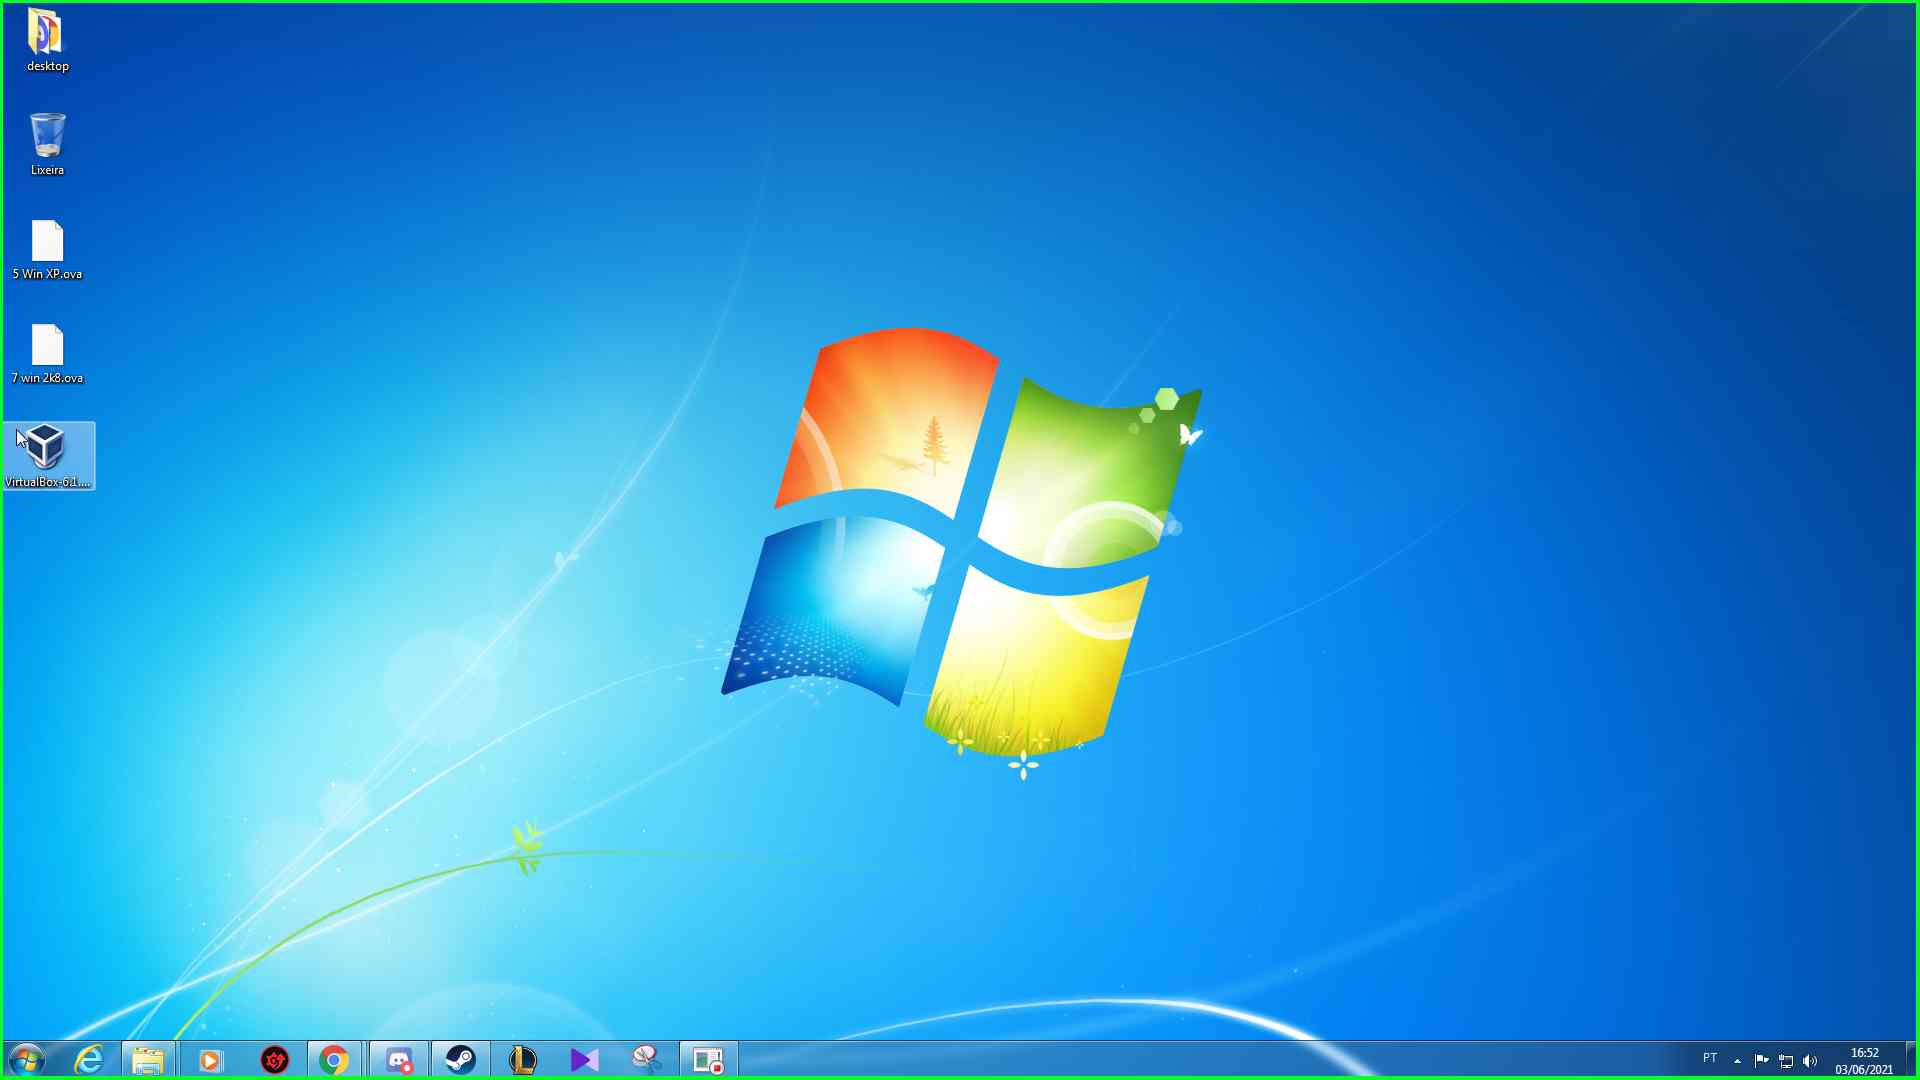
\includegraphics[width=\linewidth]{images/instalacao_virtualbox/001.png}
\end{figure}

\begin{figure}[H]
    \centering
    \caption{Clique \textbf{Executar}}
    \label{fig:22}
    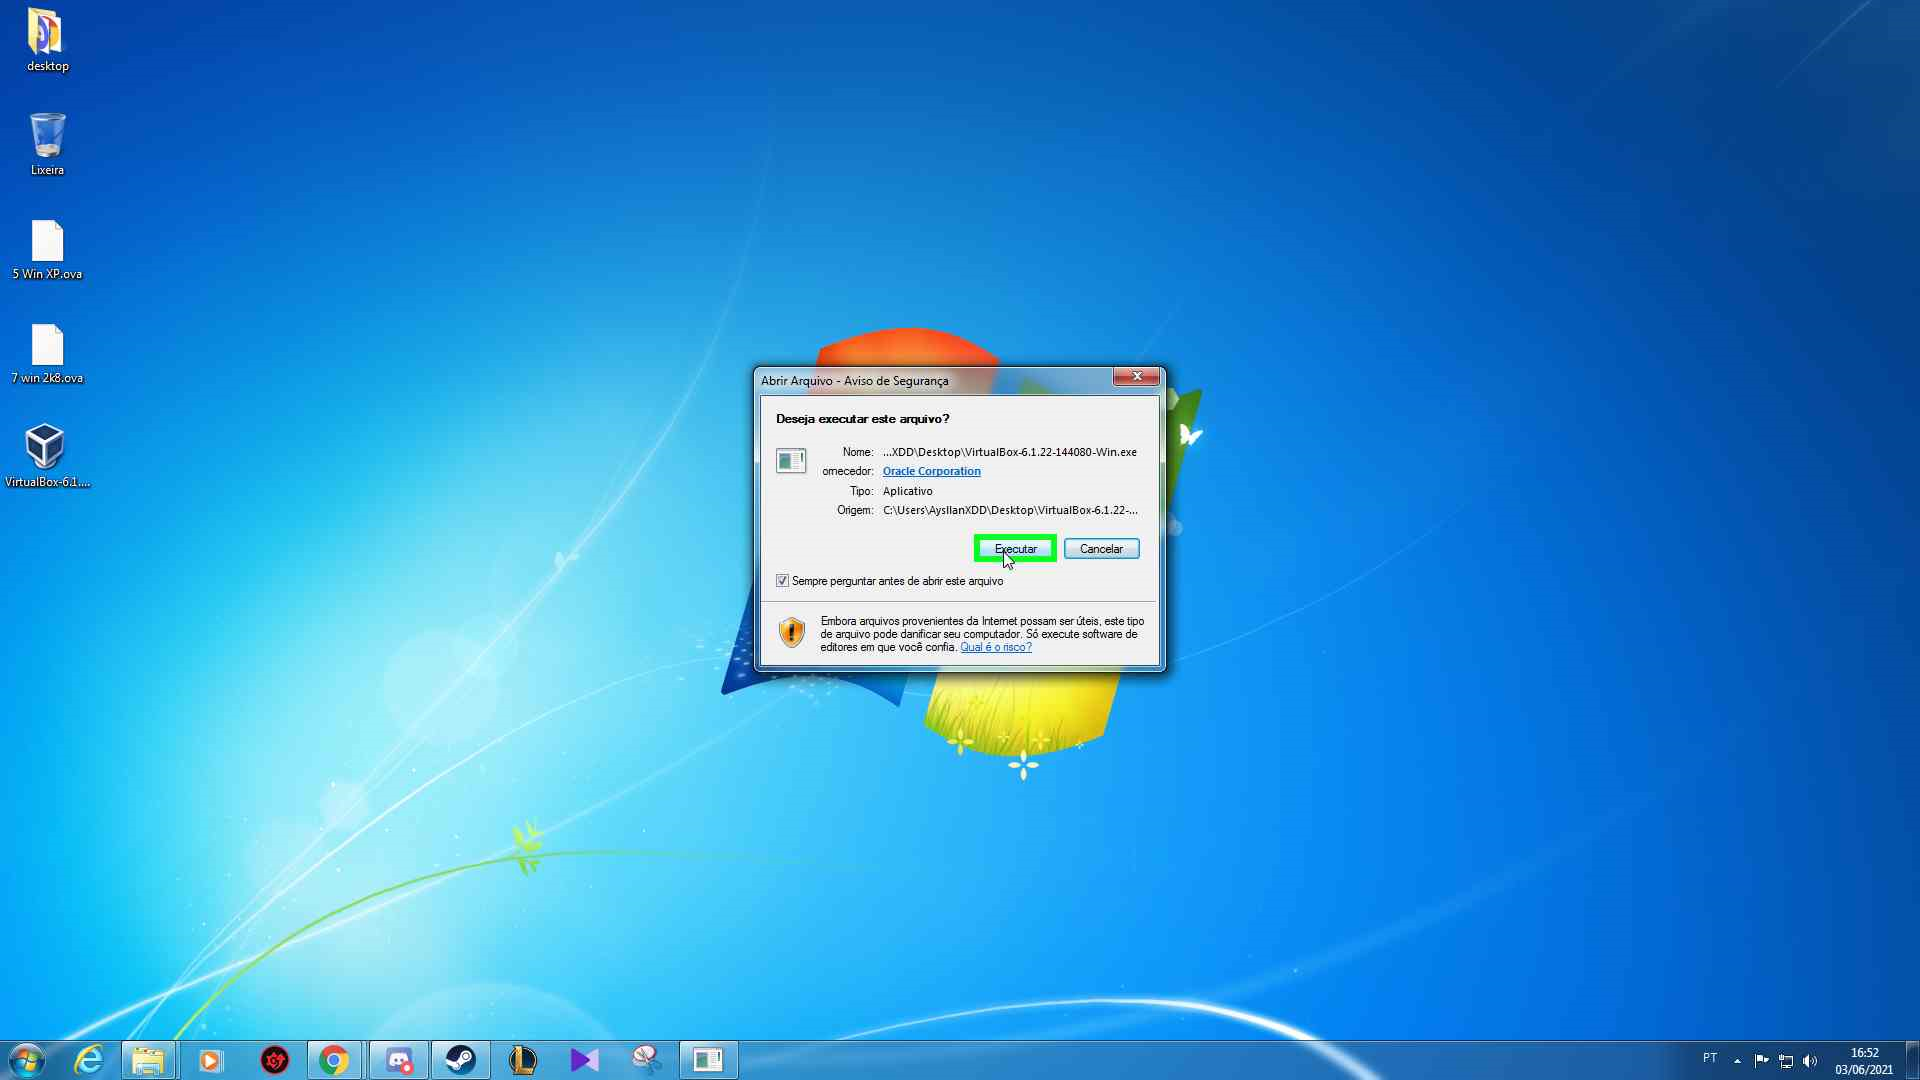
\includegraphics[width=\linewidth]{images/instalacao_virtualbox/002.png}
\end{figure}

\begin{figure}[H]
    \centering
    \caption{Clique \textbf{Next}}
    \label{fig:23}
    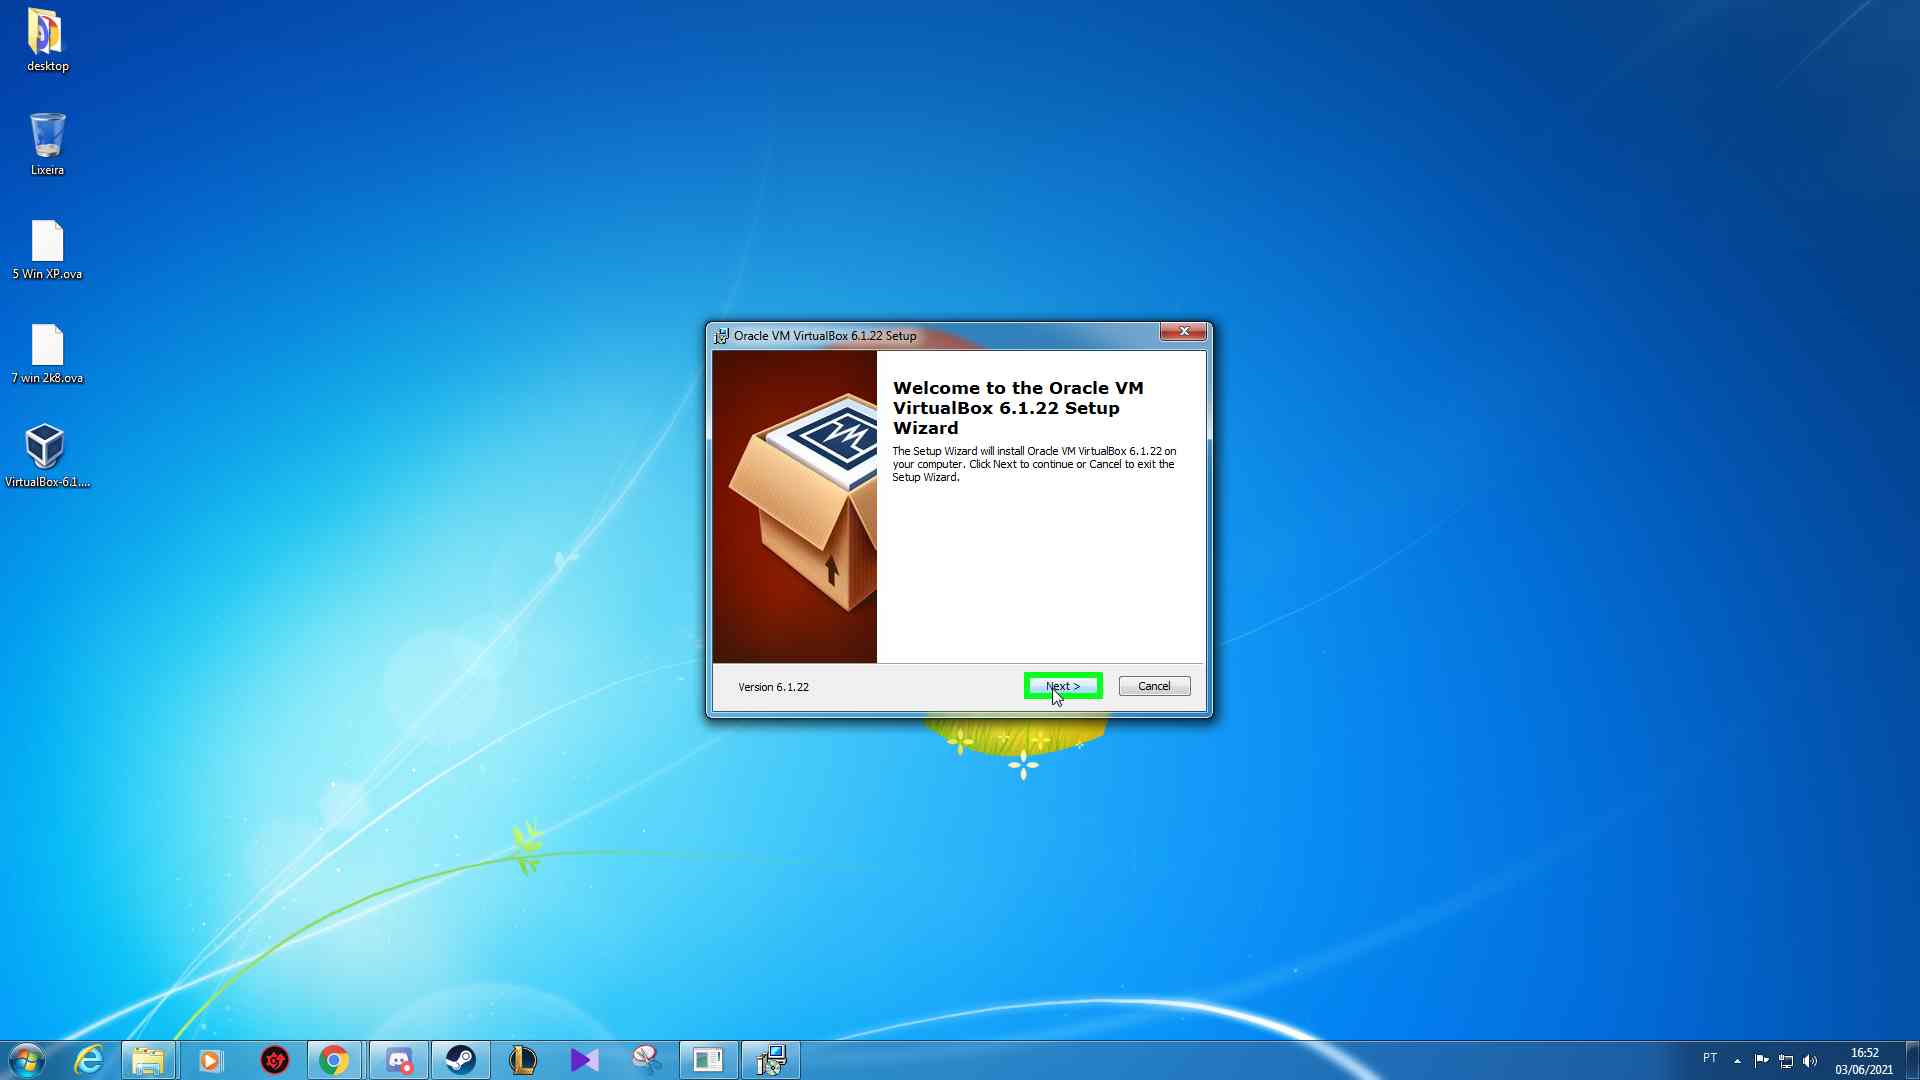
\includegraphics[width=\linewidth]{images/instalacao_virtualbox/003.png}
\end{figure}

\begin{figure}[H]
    \centering
    \caption{Clique \textbf{Next}}
    \label{fig:24}
    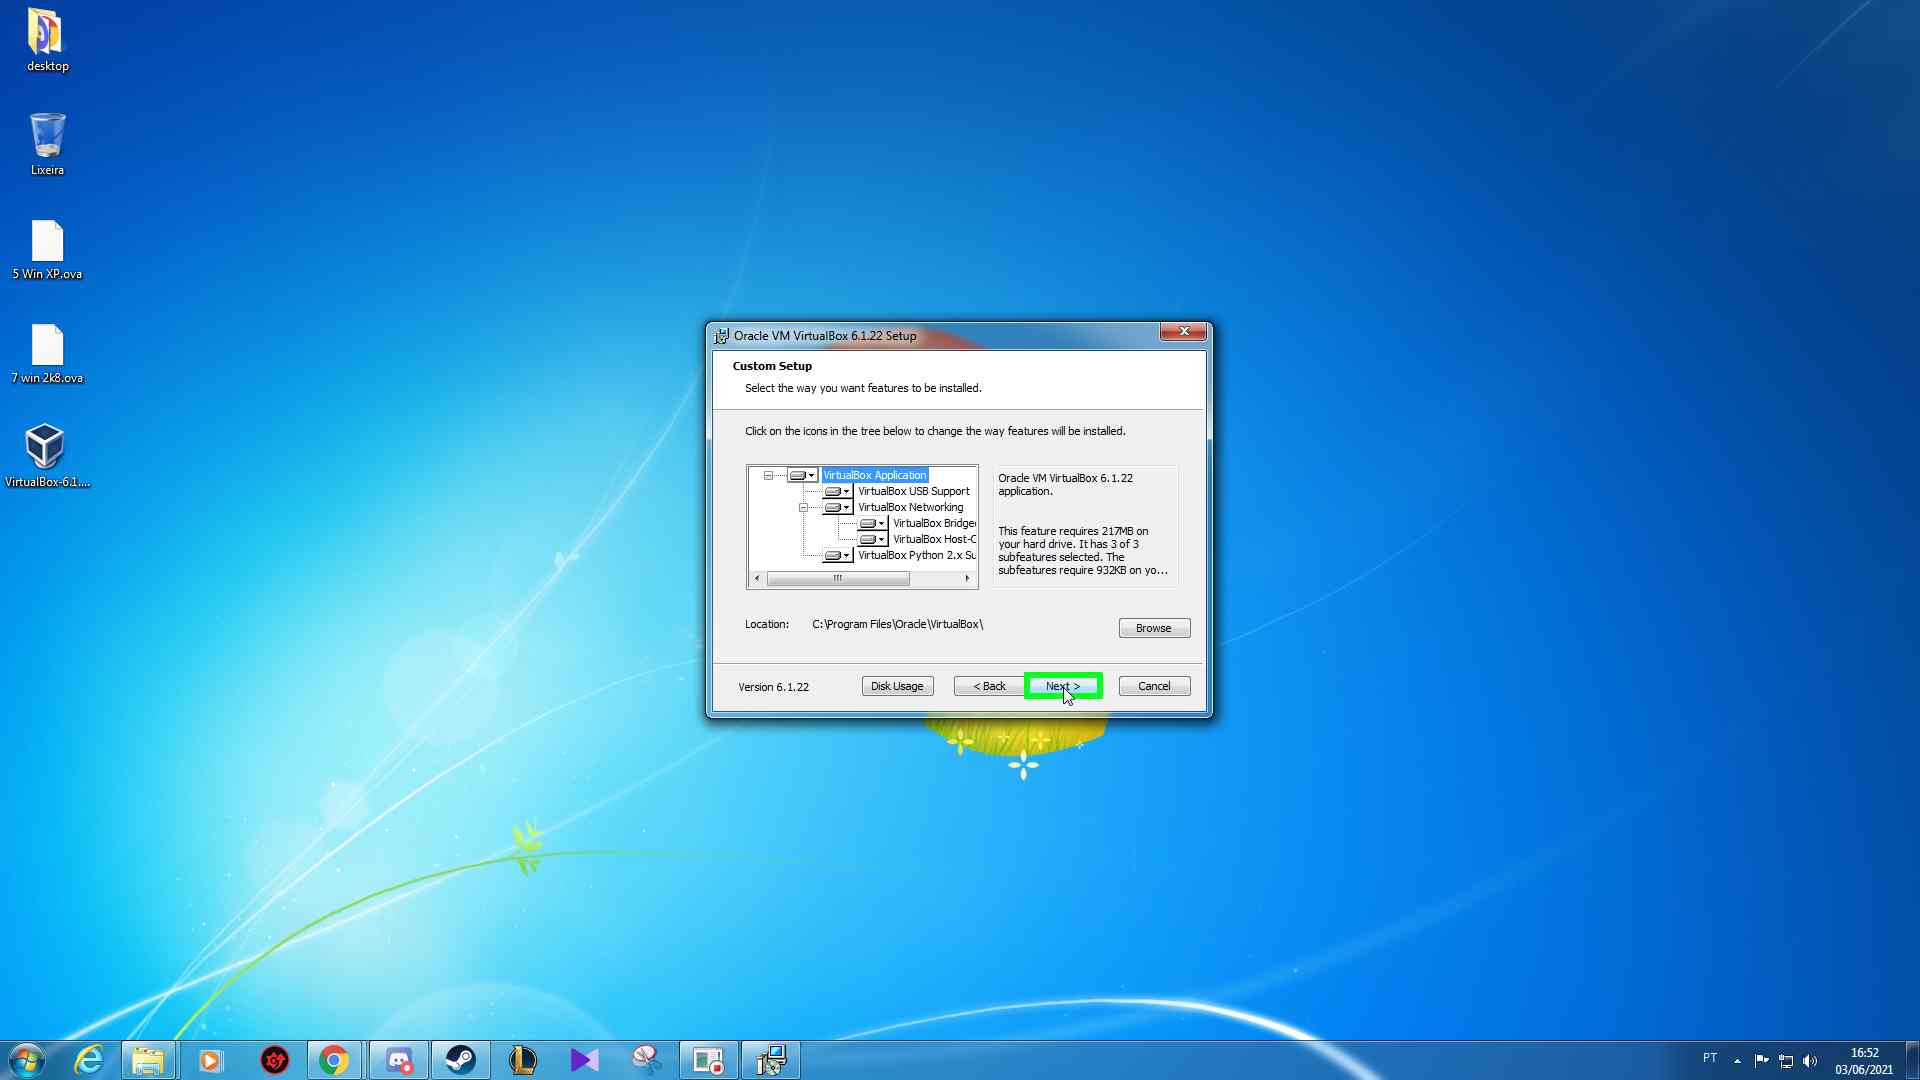
\includegraphics[width=\linewidth]{images/instalacao_virtualbox/004.png}
\end{figure}

\begin{figure}[H]
    \centering
    \caption{Clique \textbf{Next}}
    \label{fig:25}
    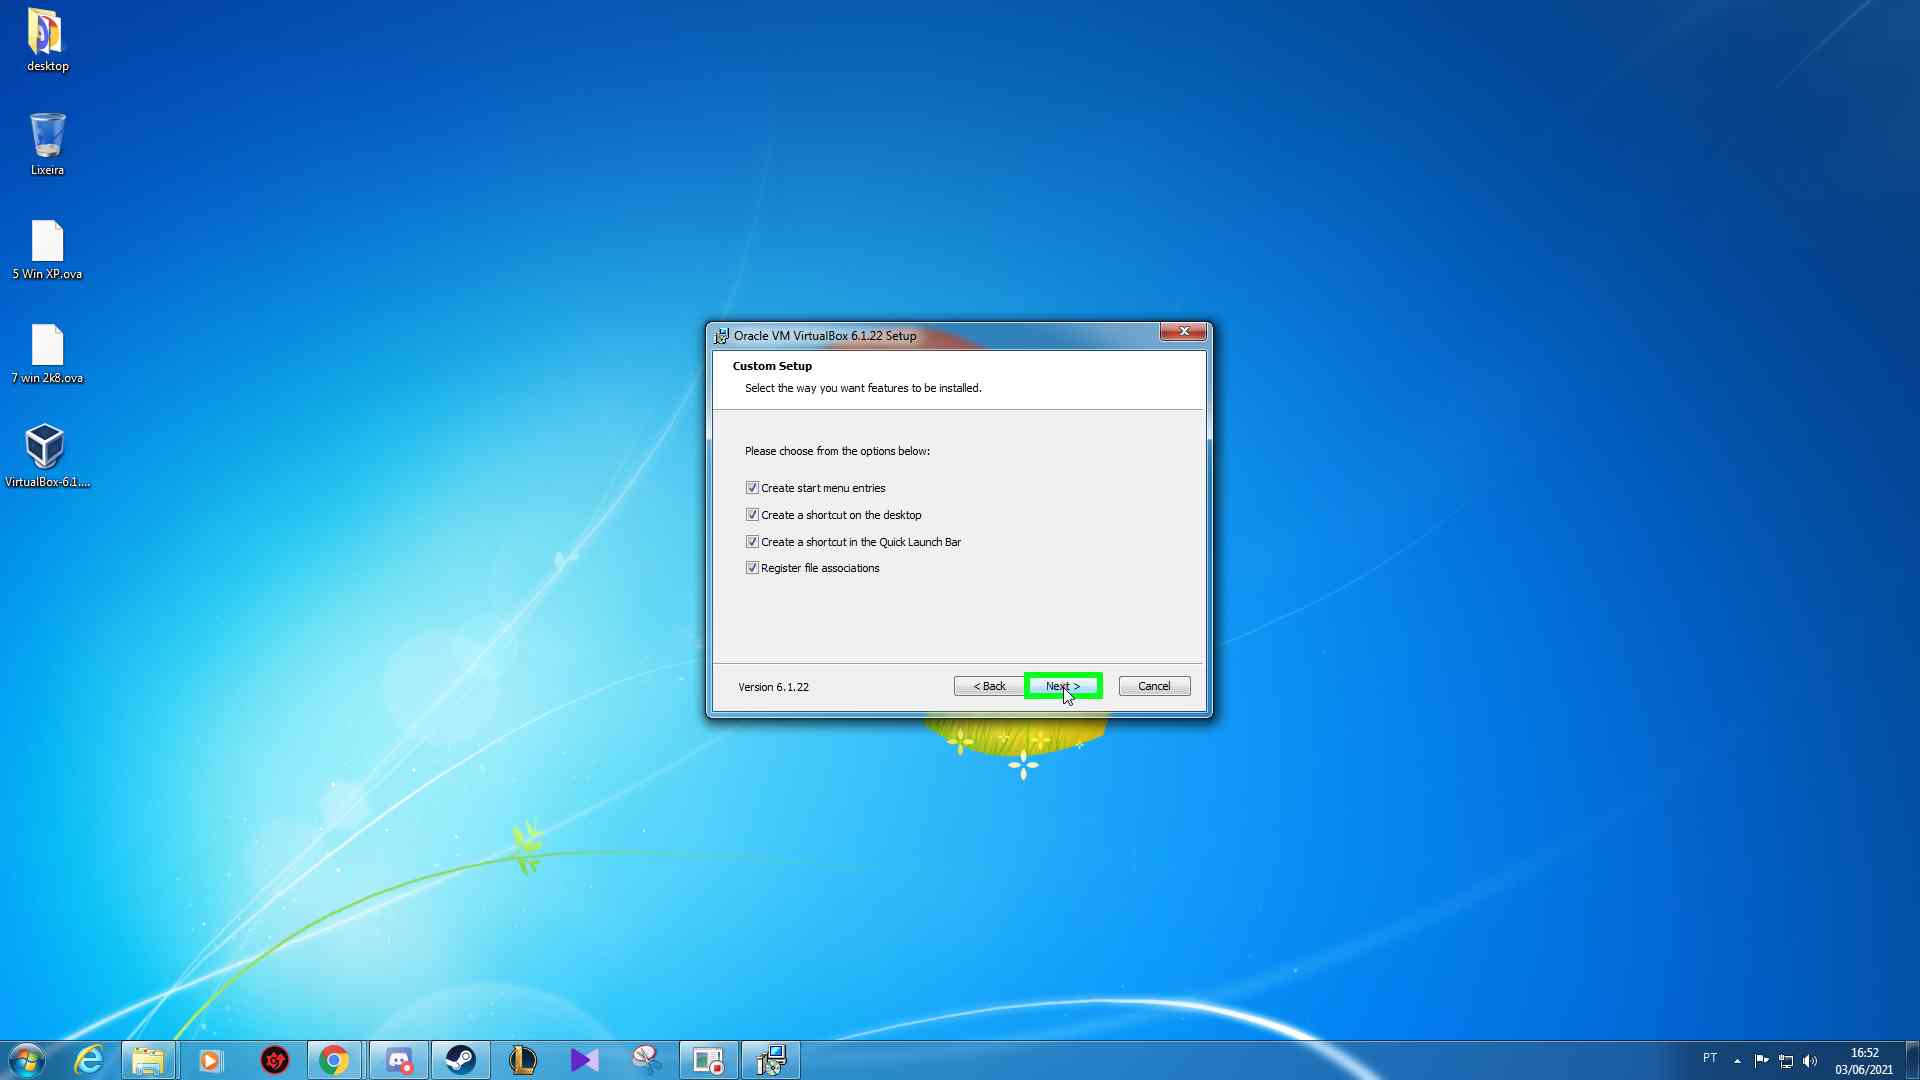
\includegraphics[width=\linewidth]{images/instalacao_virtualbox/005.png}
\end{figure}

\begin{figure}[H]
    \centering
    \caption{Clique \textbf{Yes}}
    \label{fig:26}
    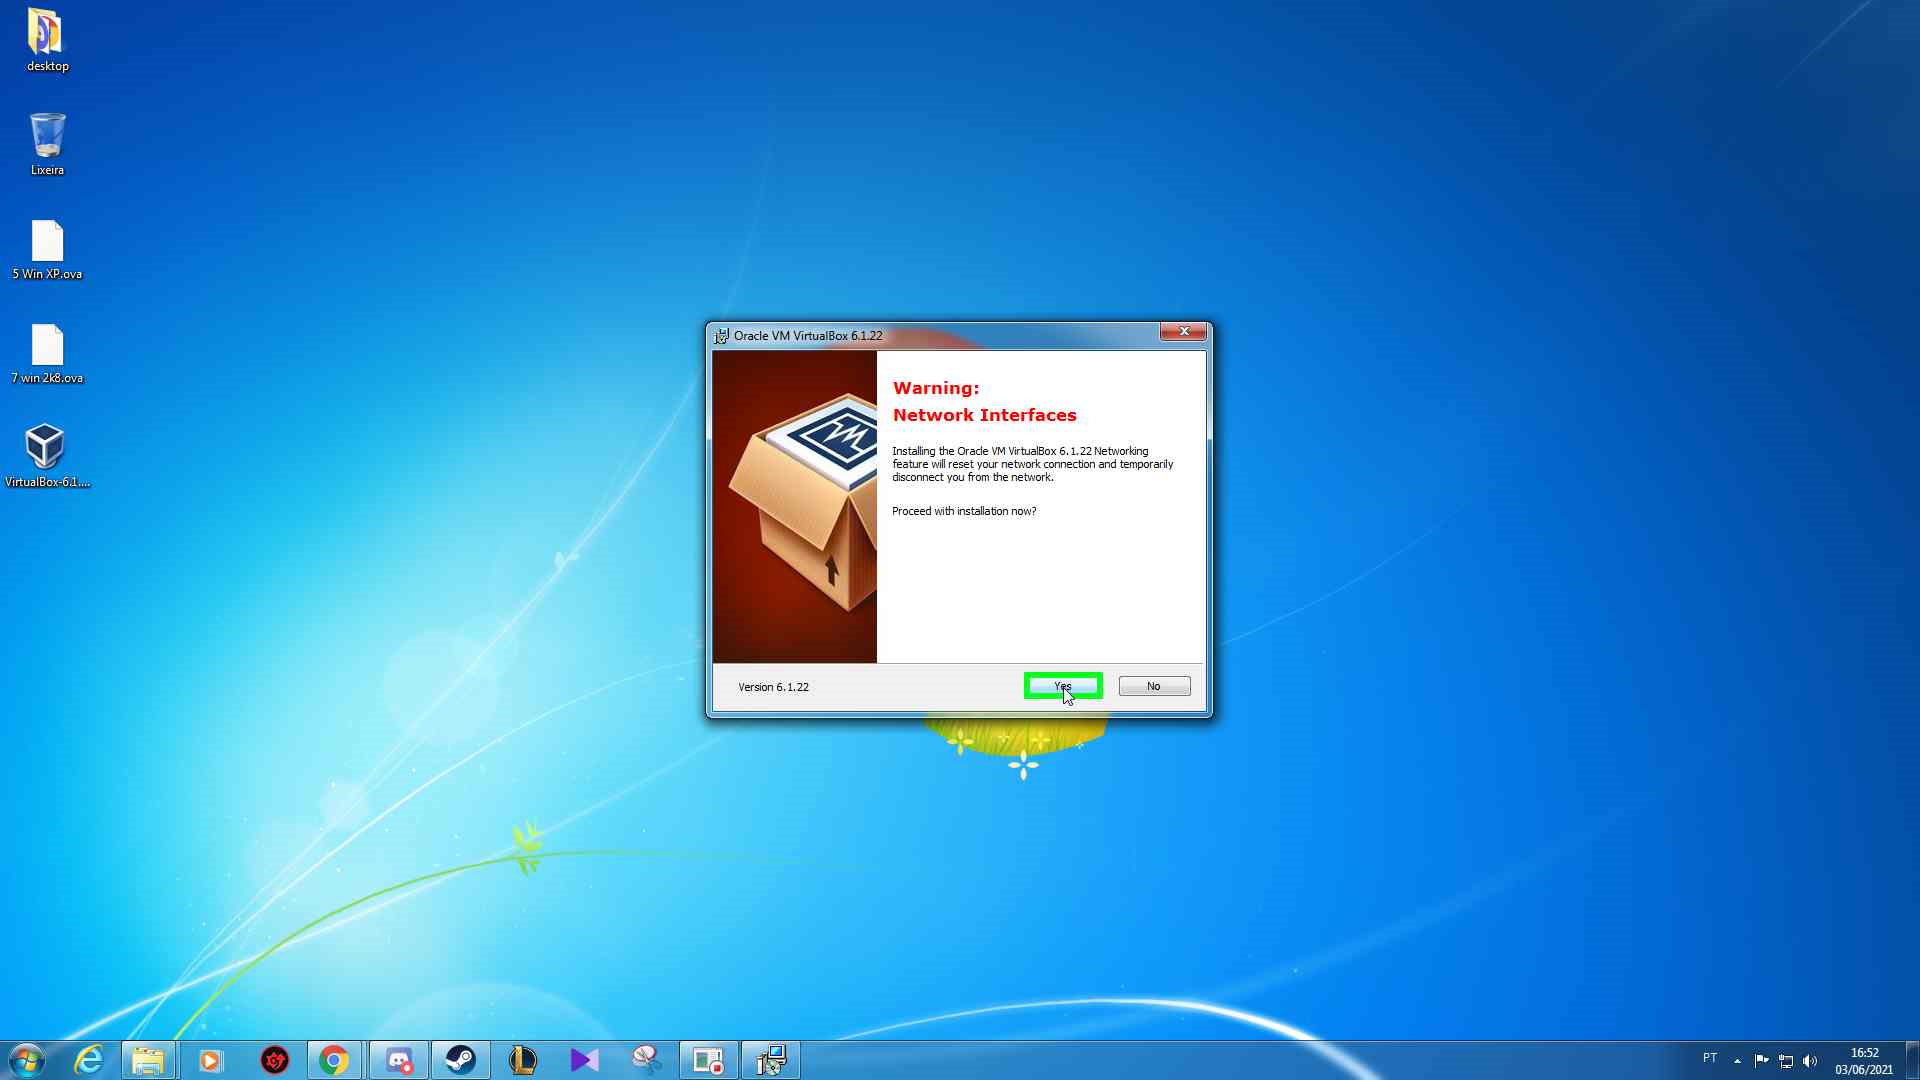
\includegraphics[width=\linewidth]{images/instalacao_virtualbox/006.png}
\end{figure}

\begin{figure}[H]
    \centering
    \caption{Clique \textbf{Install}}
    \label{fig:27}
    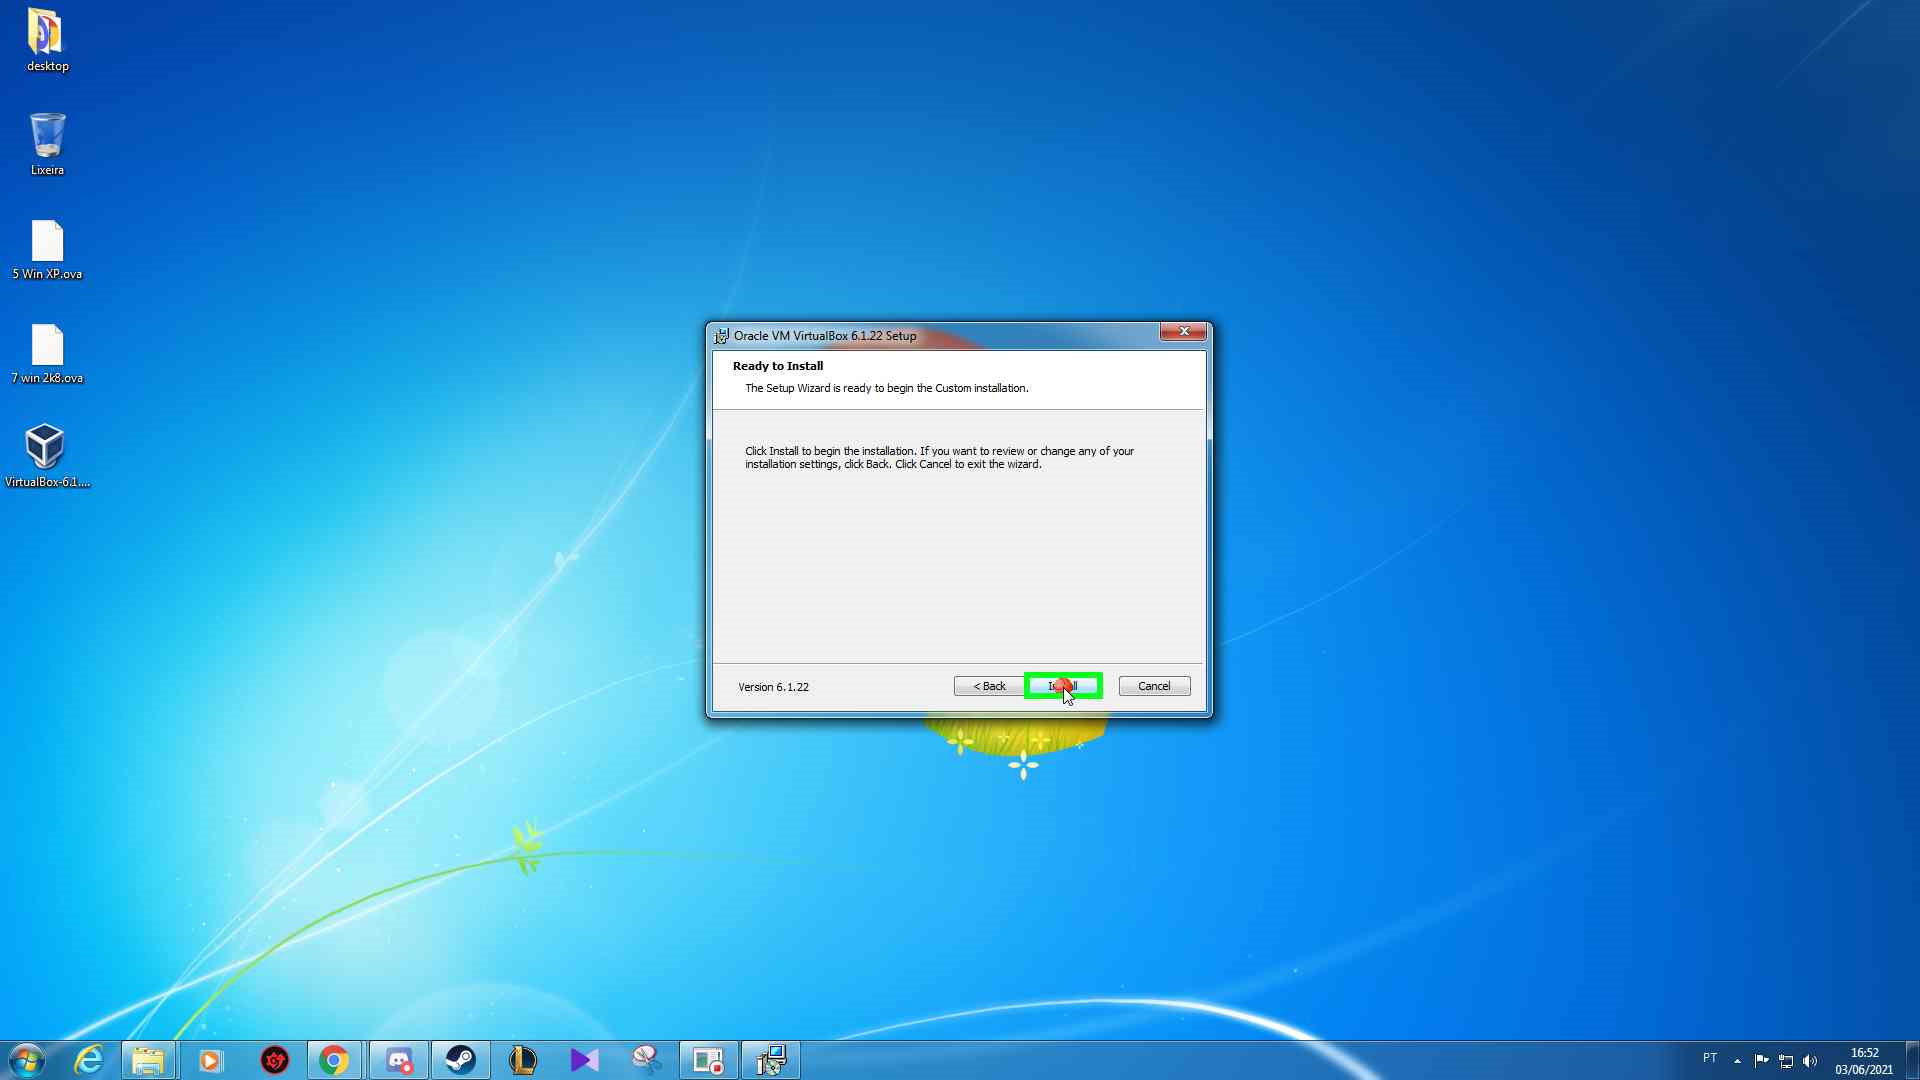
\includegraphics[width=\linewidth]{images/instalacao_virtualbox/007.png}
\end{figure}

\begin{figure}[H]
    \centering
    \caption{Clique \textbf{Finish}}
    \label{fig:28}
    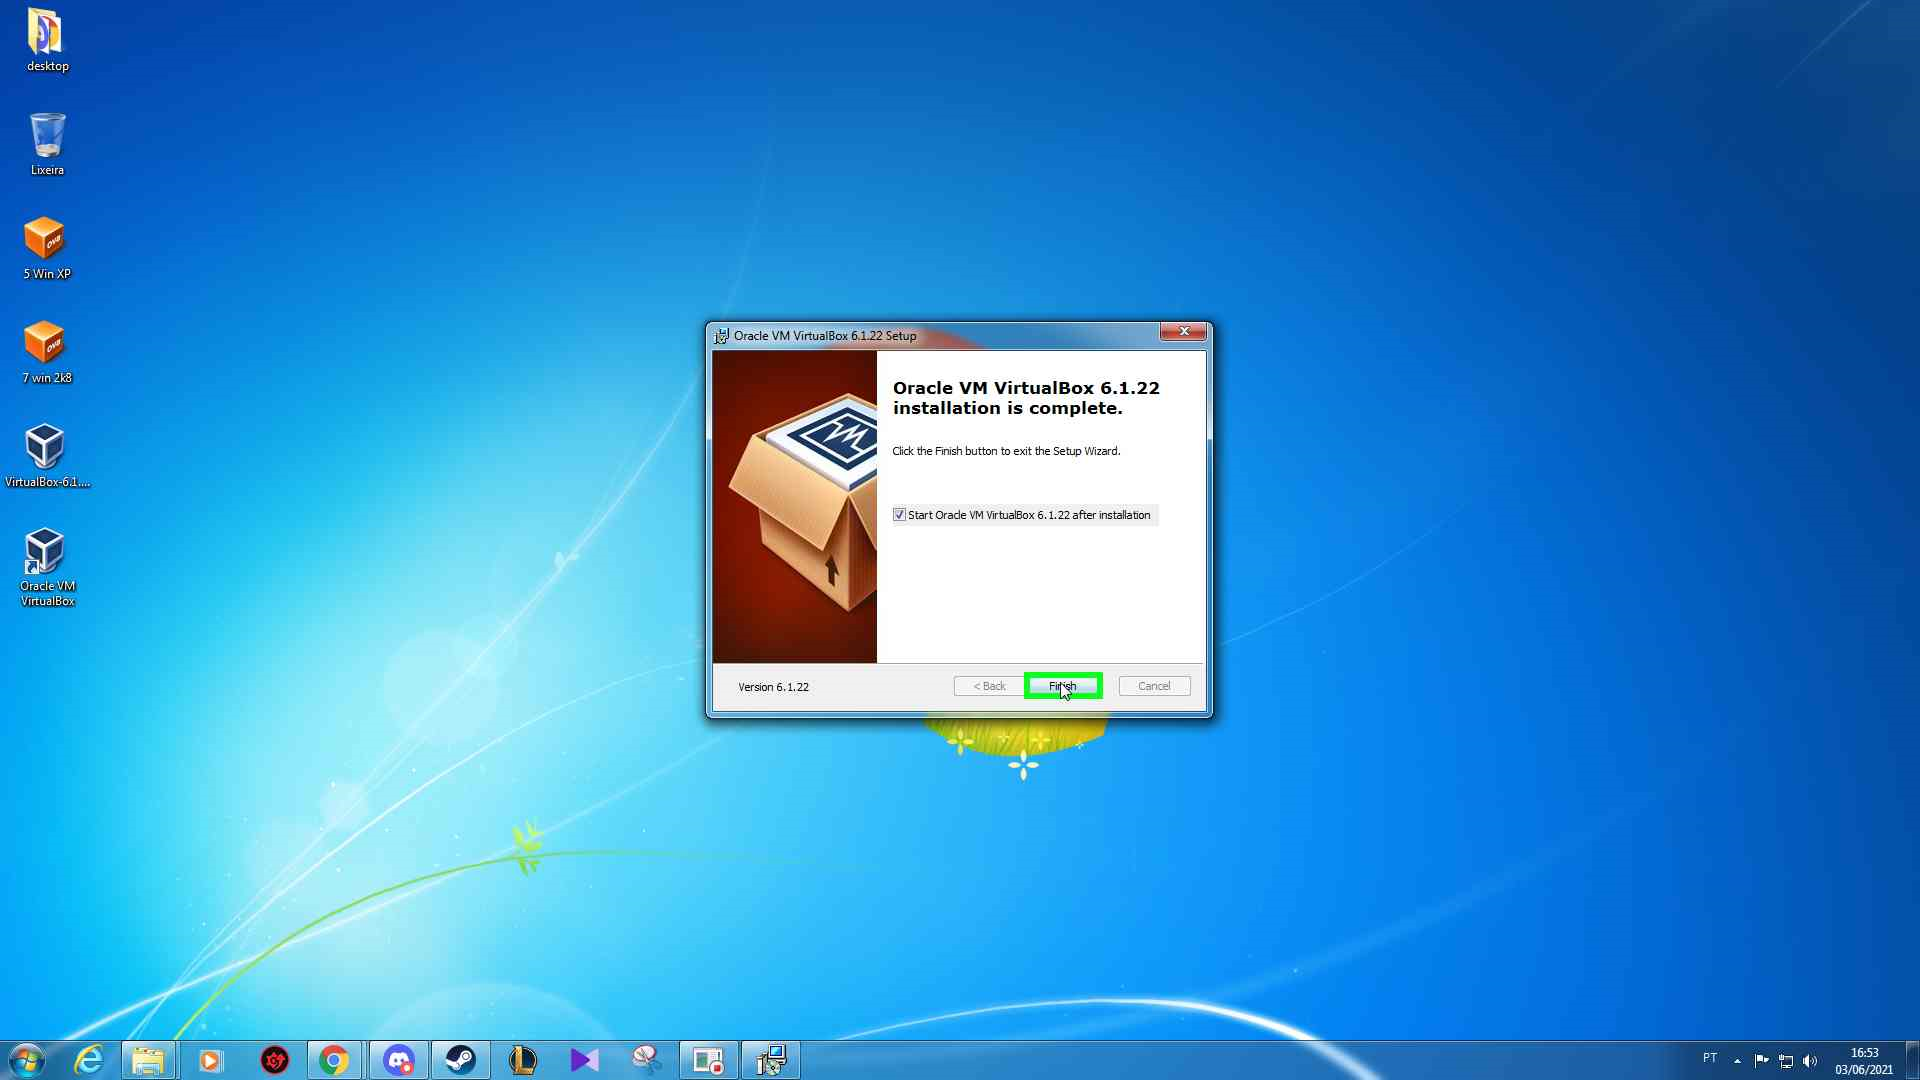
\includegraphics[width=\linewidth]{images/instalacao_virtualbox/008.png}
\end{figure}



\section{ATIVAÇÃO DAS MÁQUINAS VIRTUAIS}
Através do \textbf{Virtual Box} devemos importar os arquivos \textbf{.ova} baixados anteriormente. Clique em \textbf{Importar Appliance} (Figura \ref{fig:31}).Em seguida procure o diretório onde estão os arquivos \textbf{.ova} (Figura \ref{fig:32}). Selecione o arquivo \textbf{5 Win XP} (Figura \ref{fig:33}), após ter selecionado clique em \textbf{Próximo(N)} para continuar(Figura \ref{fig:34}) e na próxima página(Figura \ref{fig:35}) clique em \textbf{Importar}. Em seguida aparecerá uma tela de carregamento(Figura \ref{fig:36}), agora é só esperar terminar de carregar.

\par Repira o mesmo processo com o \textbf{.ova} do \textbf{7 win 2k8}.

\begin{figure}[H]
    \centering
    \caption{Clique em \textbf{Importar Appliance}}
    \label{fig:31}
    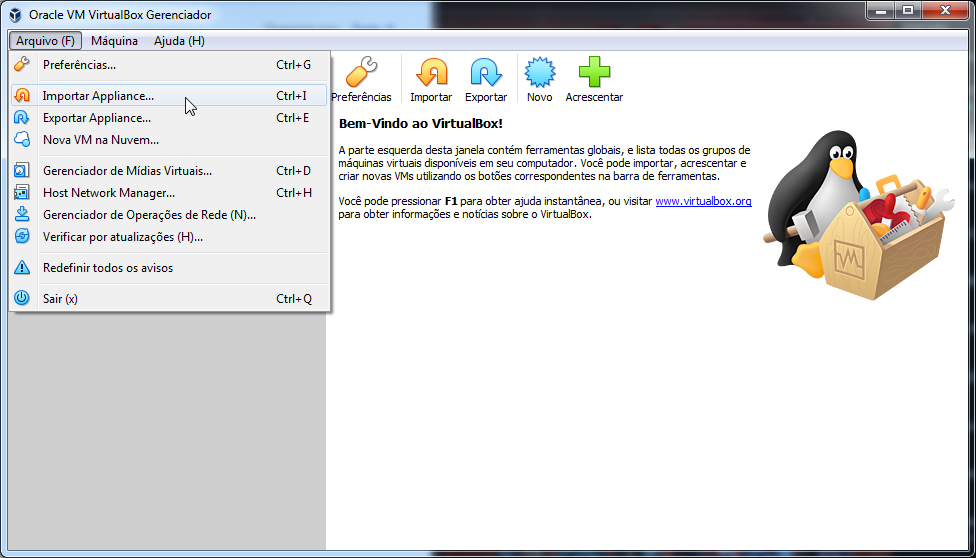
\includegraphics[width=\linewidth]{images/ativacao_das_maquinas_virtuais/001.png}
\end{figure}
\begin{figure}[H]
    \centering
    \caption{Busque o dirtório}
    \label{fig:32}
    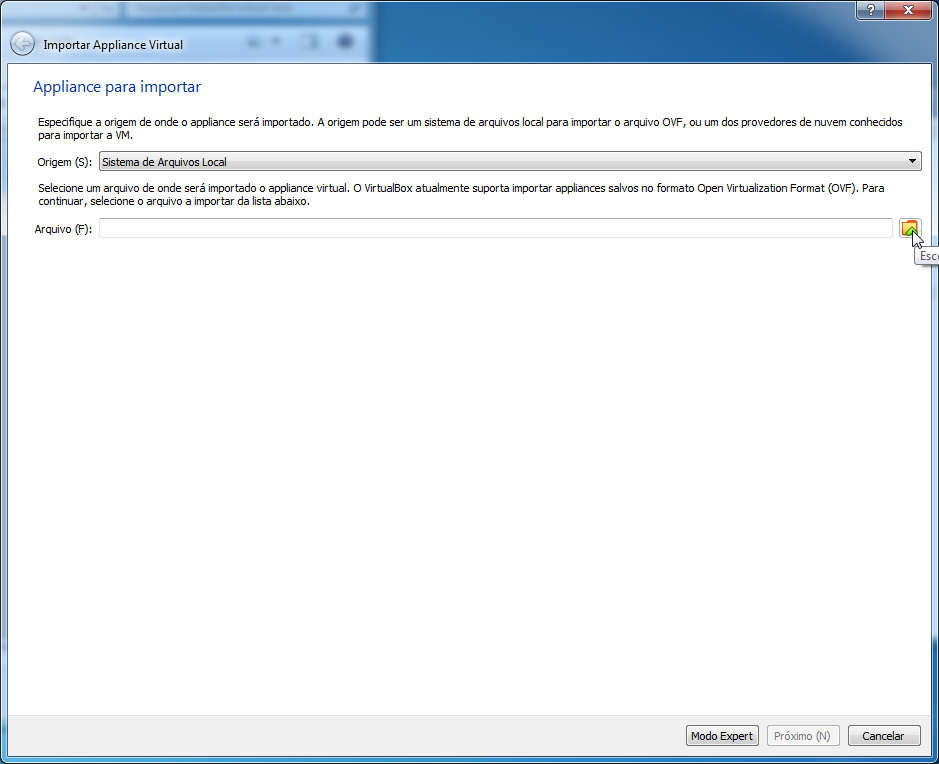
\includegraphics[width=\linewidth]{images/ativacao_das_maquinas_virtuais/002.png}
\end{figure}
\begin{figure}[H]
    \centering
    \caption{Selecione o arquivo \textbf{.ova}}
    \label{fig:33}
    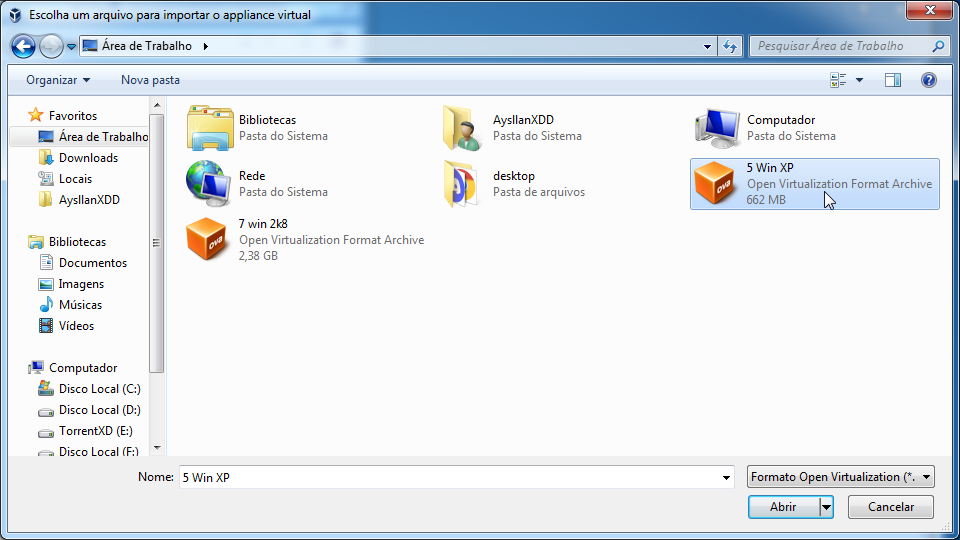
\includegraphics[width=\linewidth]{images/ativacao_das_maquinas_virtuais/003.png}
\end{figure}
\begin{figure}[H]
    \centering
    \caption{Clique em \textbf{Próximo(N)}}
    \label{fig:34}
    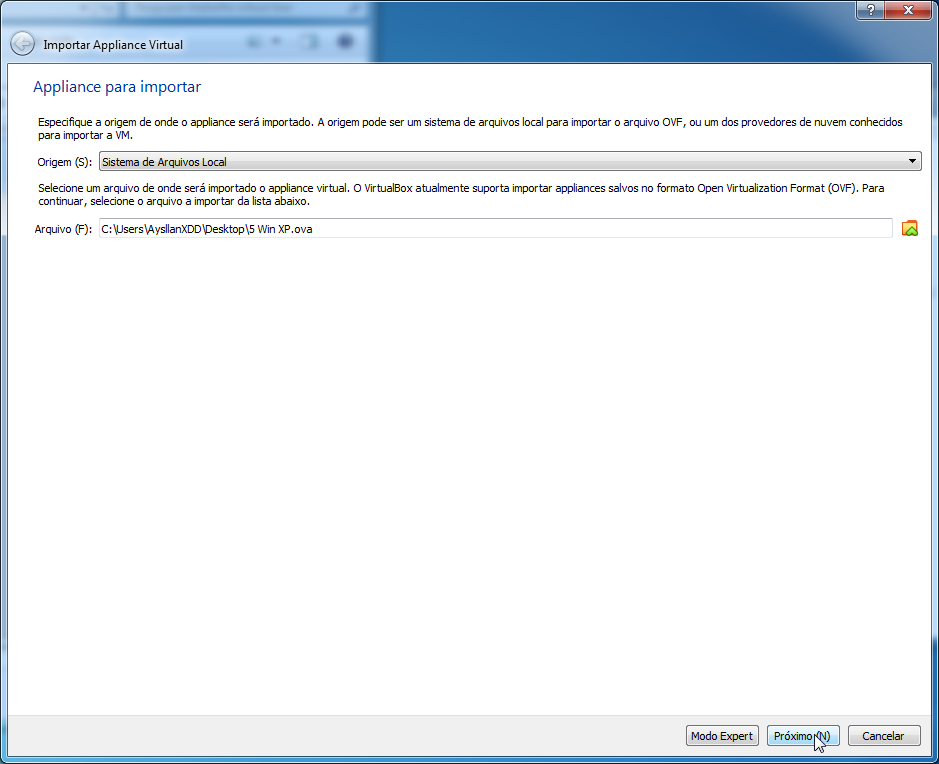
\includegraphics[width=\linewidth]{images/ativacao_das_maquinas_virtuais/004.png}
\end{figure}
\begin{figure}[H]
    \centering
    \caption{Clique em \textbf{Importar}}
    \label{fig:35}
    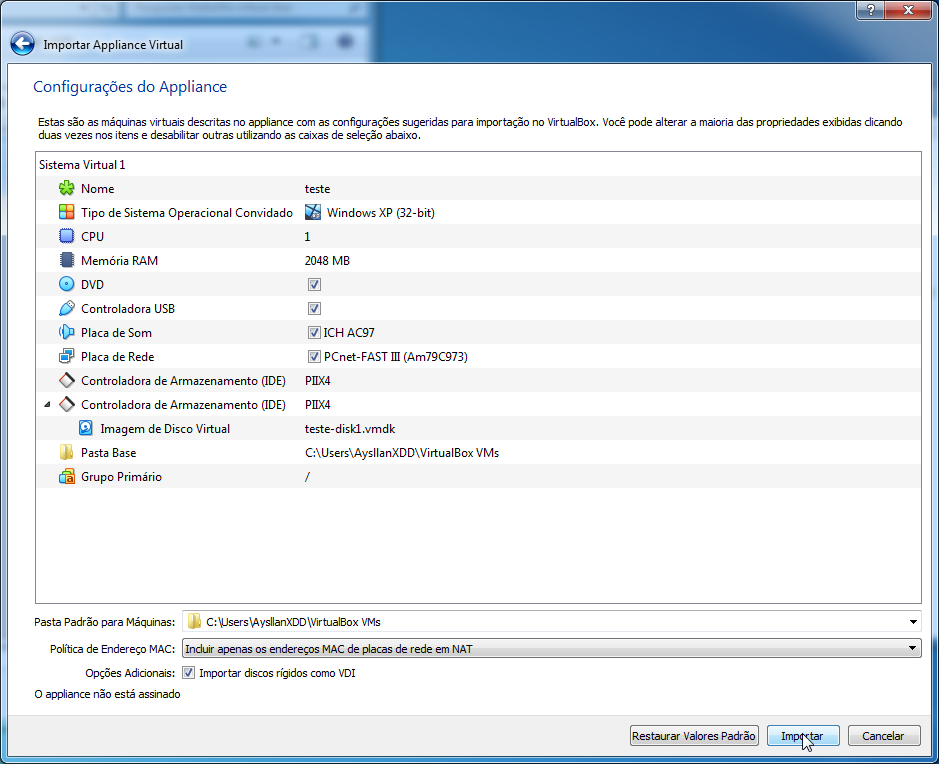
\includegraphics[width=\linewidth]{images/ativacao_das_maquinas_virtuais/005.png}
\end{figure}
\begin{figure}[H]
    \centering
    \caption{Aguarde tela de carregamento}
    \label{fig:36}
    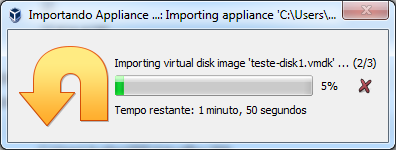
\includegraphics[width=\linewidth]{images/ativacao_das_maquinas_virtuais/006.png}
\end{figure}


\subsection{Configuração inicial das máquinas virtuais}
\par Para configurar selecione a maquina que deseja e clique em \textbf{Configurações} (Figura \ref{fig:317}), coloque o nome que desejar (Figura \ref{fig:318}). Na tela de \textbf{Monitor} coloque a \textbf{Memória de Vídeo} no máximo (Figura \ref{fig:319}).Em \textbf{sistemas} mudar a \textbf{Memória Base} para \textbf{2048 MB} (Figura \ref{fig:3110}).Em \textbf{Rede} mudar no campo \textbf{Conectato a: NAT} para \textbf{Rede interna} (Figura \ref{fig:3111}). Na tela \textbf{Pastas Compartilhadas} se tiver algum conteudo basta selecionar e clicar em excluir (Figura \ref{fig:3112})

\par Repita o processo com a segunda maquina.

\par Agora iremos instalar os drivers do virtual box no Win XP, inicie o Win XP (Figura \ref{fig:3114}). Após iniciar clique em \textbf{Inserir imagem de CD} (Figura \ref{fig:3115}), abrindo uma janela clique em \textbf{Next} (Figura \ref{fig:3116}), novamente em \textbf{Next} (Figura \ref{fig:3117}), agora clique em \textbf{Install} (Figura \ref{fig:3118}). Aparecerá uma tela de aviso, basta apertar em \textbf{Continuar assim mesmo} (Figura \ref{fig:3119}), novamente em \textbf{Continuar assim mesmo} (Figura \ref{fig:3120}) e mais uma vez em \textbf{Continuar assim mesmo} (Figura \ref{fig:3121}). clique em \textbf{Finish} e a maquina será reiniciada (Figura \ref{fig:3122}).

\par É importante repetirmos o passo anterior, porém agora no \textbf{2k8-Server}, inicie o 2k8-Server (Figura \ref{fig:3124}), inicie o windows normalmente (Figura \ref{fig:3125}), após iniciar clique em \textbf{OK} (Figura \ref{fig:3126}), agora escolha uma senha de sua preferência e avance (Figura \ref{fig:3127}). Ao entrar ira aparecer um tela de ativação, basta ignorar clicando em \textbf{Ativar mais tarde} ou em \textbf{Cancelar} (Figura \ref{fig:3129}). Va em \textbf{Dispositivos} e \textbf{Inserir imagem de CD dos Adicionais para Convidado} (Figura \ref{fig:3130}), abrindo uma janela pode executar (Figura \ref{fig:3131}), começando clique em \textbf{Next} (Figura \ref{fig:3132}), clique em \textbf{Next} (Figura \ref{fig:3133}), agora clique em \textbf{Install} (Figura \ref{fig:3134}), aparecerá uma tela de aviso, basta clicar em \textbf{Instalar este software de driver mesmo assim} (Figura \ref{fig:3135}), clique novamente em \textbf{Instalar este software de driver mesmo assim} (Figura \ref{fig:3136}), quando estiver quase terminando ira dar erro, mas não se preocupe, é só clicar em \textbf{Cancel} (Figura \ref{fig:3137}), abrindo uma janela de erro clique em \textbf{OK} (Figura \ref{fig:3138}). Terminando va em \textbf{Iniciar} e \textbf{Reiniciar} (Figura \ref{fig:3139}), escreva algo na janela de \textbf{Comentário:} e clique em \textbf{OK} (Figura \ref{fig:3141}), após reiniciar digite \textbf{CTRL(Dieito) + DEL} (Figura \ref{fig:3142}), digite sua senha e avance (Figura \ref{fig:3144}), Clique em \textbf{Ativar mais tarde} ou \textbf{Cancel} (Figura \ref{fig:3145}). E pronto (Figura \ref{fig:3146}).


\begin{figure}[H]
    \centering
    \caption{Clique em \textbf{Configurações}}
    \label{fig:317}
    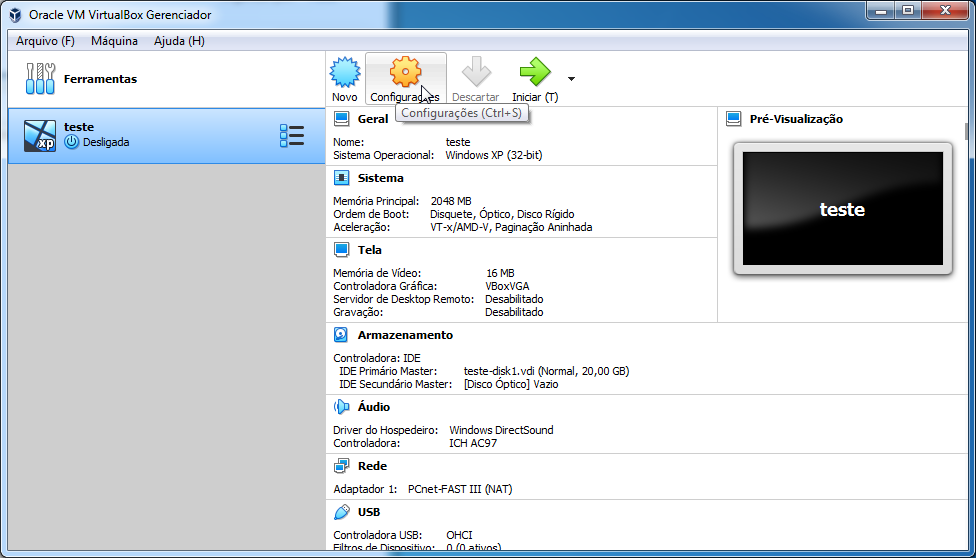
\includegraphics[width=\linewidth]{images/ativacao_das_maquinas_virtuais/configuracao_inicial_das_maquinas_virtuais/007.png}
\end{figure}
\begin{figure}[H]
    \centering
    \caption{Clique em \textbf{Mude o nome se preferir}}
    \label{fig:318}
    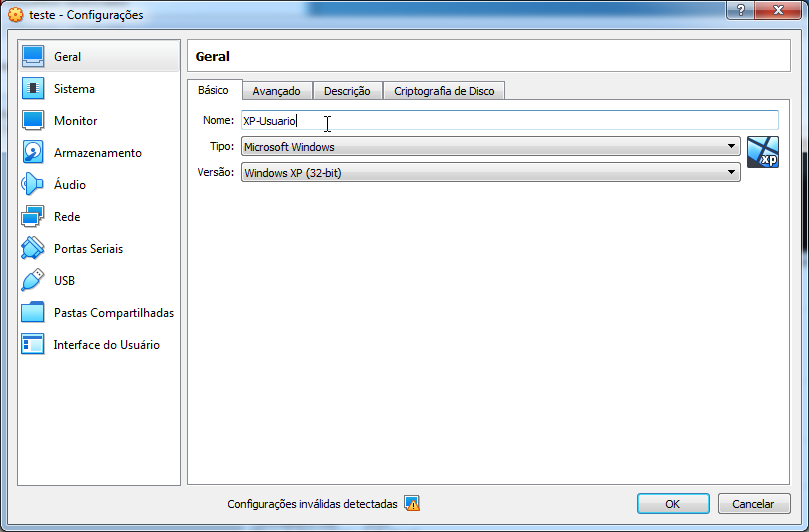
\includegraphics[width=\linewidth]{images/ativacao_das_maquinas_virtuais/configuracao_inicial_das_maquinas_virtuais/008.png}
\end{figure}
\begin{figure}[H]
    \centering
    \caption{Clique em \textbf{Mudar a memória de vídeo}}
    \label{fig:319}
    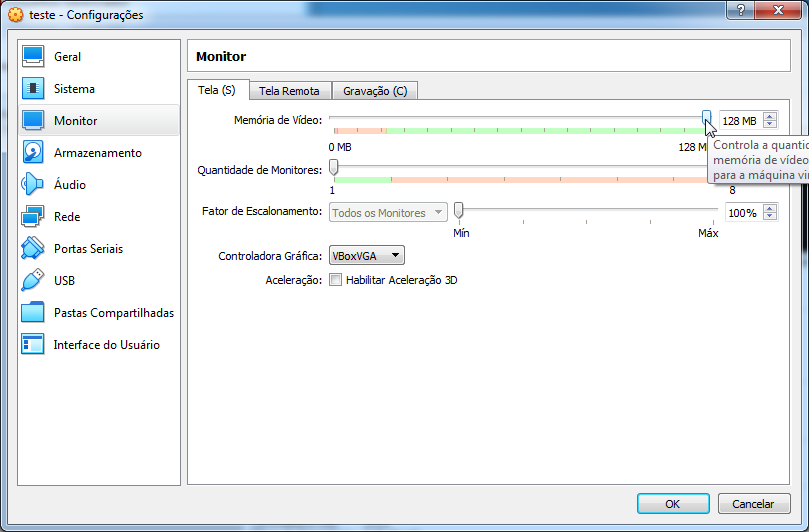
\includegraphics[width=\linewidth]{images/ativacao_das_maquinas_virtuais/configuracao_inicial_das_maquinas_virtuais/009.png}
\end{figure}
\begin{figure}[H]
    \centering
    \caption{Clique em \textbf{Mudar a memória Base}}
    \label{fig:3110}
    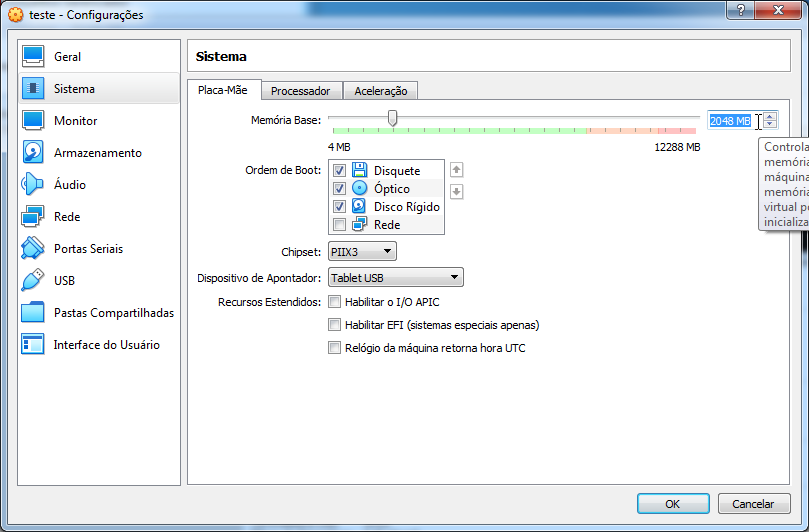
\includegraphics[width=\linewidth]{images/ativacao_das_maquinas_virtuais/configuracao_inicial_das_maquinas_virtuais/010.png}
\end{figure}
\begin{figure}[H]
    \centering
    \caption{Clique em \textbf{Mudar a conexão}}
    \label{fig:3111}
    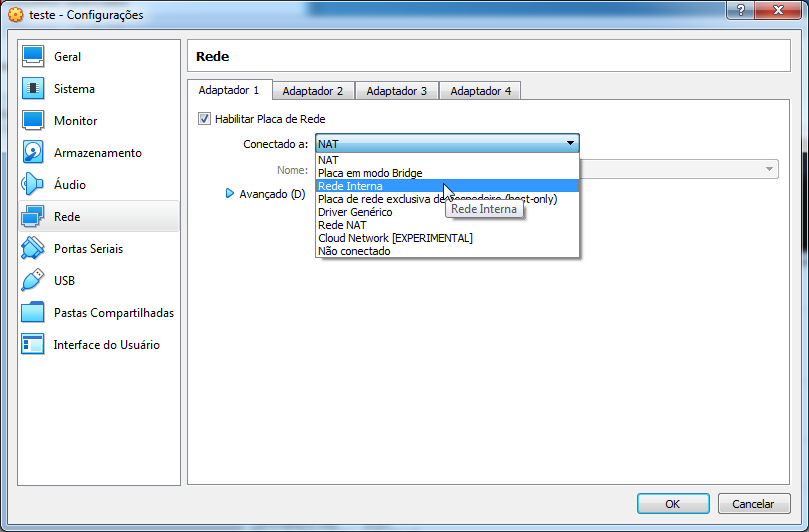
\includegraphics[width=\linewidth]{images/ativacao_das_maquinas_virtuais/configuracao_inicial_das_maquinas_virtuais/011.png}
\end{figure}
\begin{figure}[H]
    \centering
    \caption{Clique em \textbf{Excluir pasta (se tiver)}}
    \label{fig:3112}
    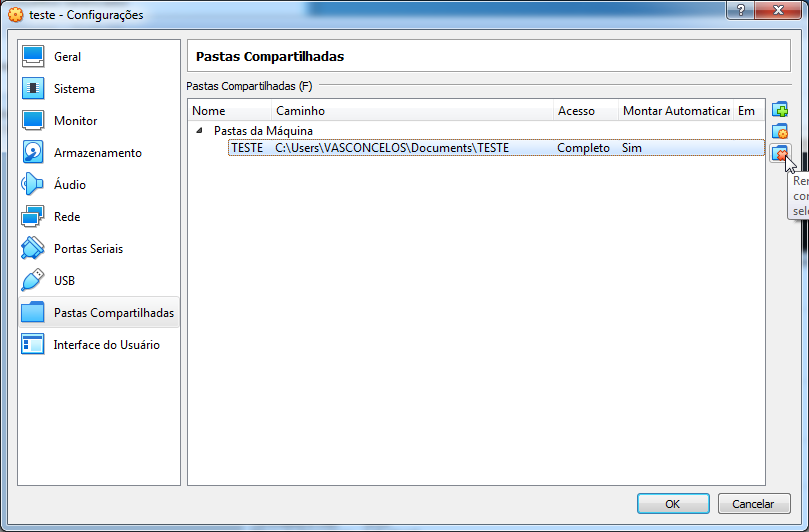
\includegraphics[width=\linewidth]{images/ativacao_das_maquinas_virtuais/configuracao_inicial_das_maquinas_virtuais/012.png}
\end{figure}
\begin{figure}[H]
    \centering
    \caption{Clique em \textbf{Inicia}}
    \label{fig:3114}
    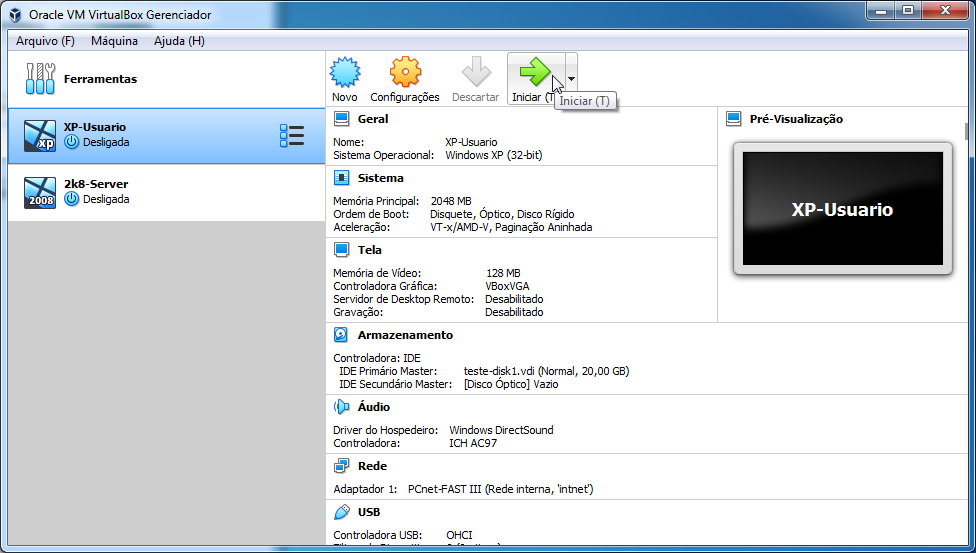
\includegraphics[width=\linewidth]{images/ativacao_das_maquinas_virtuais/configuracao_inicial_das_maquinas_virtuais/014.png}
\end{figure}
\begin{figure}[H]
    \centering
    \caption{Clique em \textbf{\textbf{Dispositivos - Inserir imagem de CD dos Adicionais para Convidado}}}
    \label{fig:3115}
    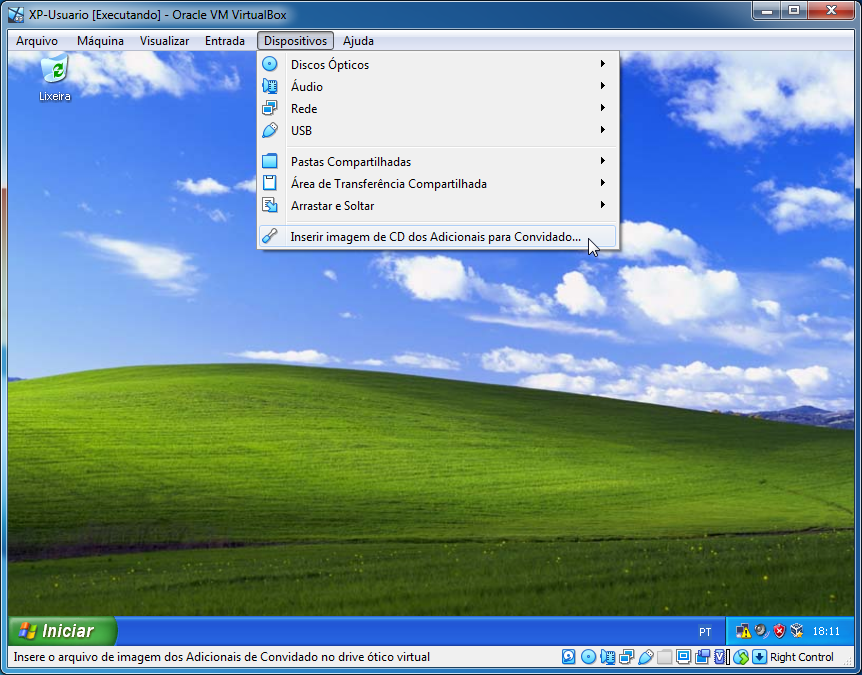
\includegraphics[width=\linewidth]{images/ativacao_das_maquinas_virtuais/configuracao_inicial_das_maquinas_virtuais/015.png}
\end{figure}
\begin{figure}[H]
    \centering
    \caption{Clique em \textbf{Next}}
    \label{fig:3116}
    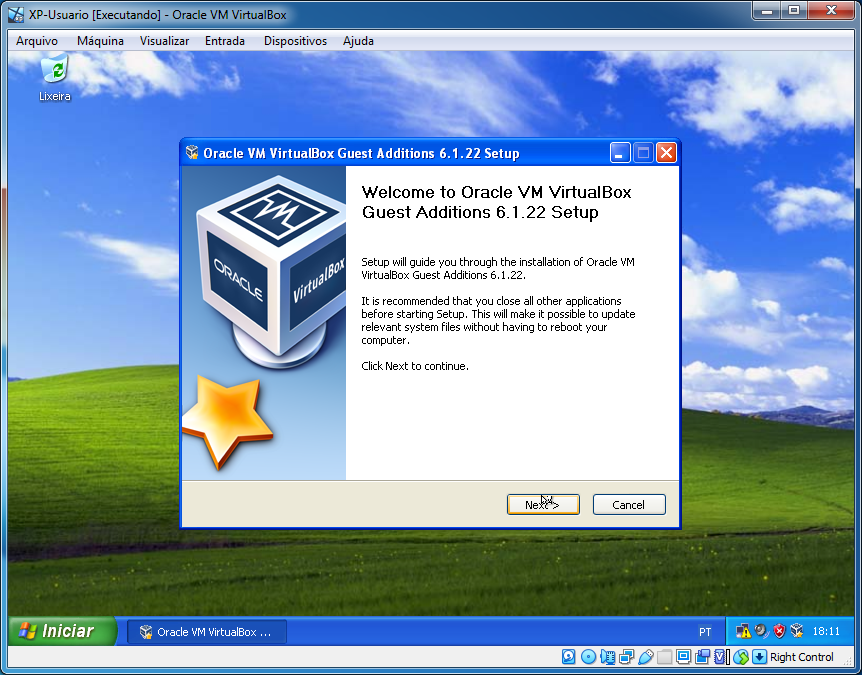
\includegraphics[width=\linewidth]{images/ativacao_das_maquinas_virtuais/configuracao_inicial_das_maquinas_virtuais/016.png}
\end{figure}
\begin{figure}[H]
    \centering
    \caption{Clique em \textbf{Next}}
    \label{fig:3117}
    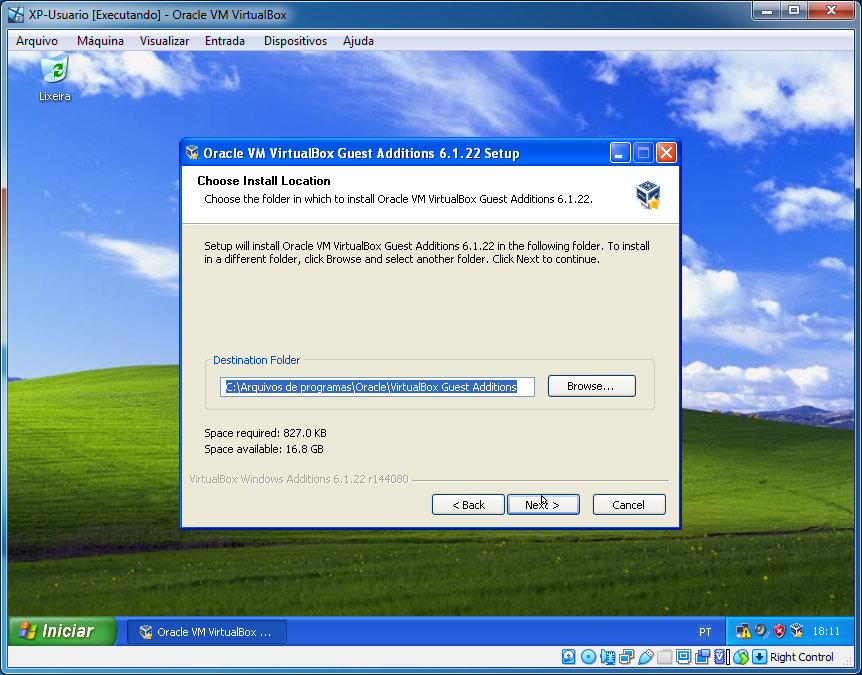
\includegraphics[width=\linewidth]{images/ativacao_das_maquinas_virtuais/configuracao_inicial_das_maquinas_virtuais/017.png}
\end{figure}
\begin{figure}[H]
    \centering
    \caption{Clique em \textbf{Install}}
    \label{fig:3118}
    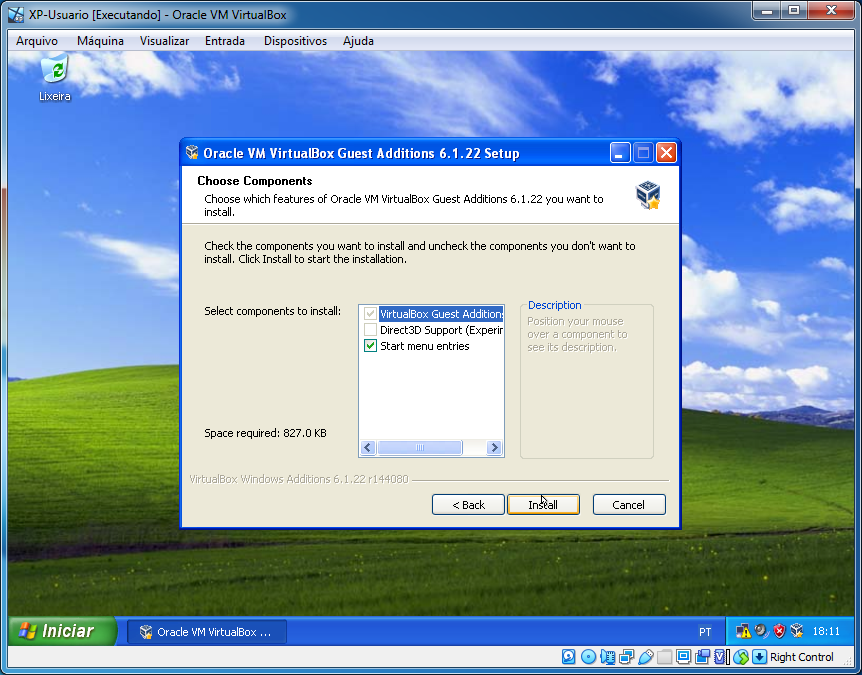
\includegraphics[width=\linewidth]{images/ativacao_das_maquinas_virtuais/configuracao_inicial_das_maquinas_virtuais/018.png}
\end{figure}
\begin{figure}[H]
    \centering
    \caption{Clique em \textbf{Continuar assim mesmo}}
    \label{fig:3119}
    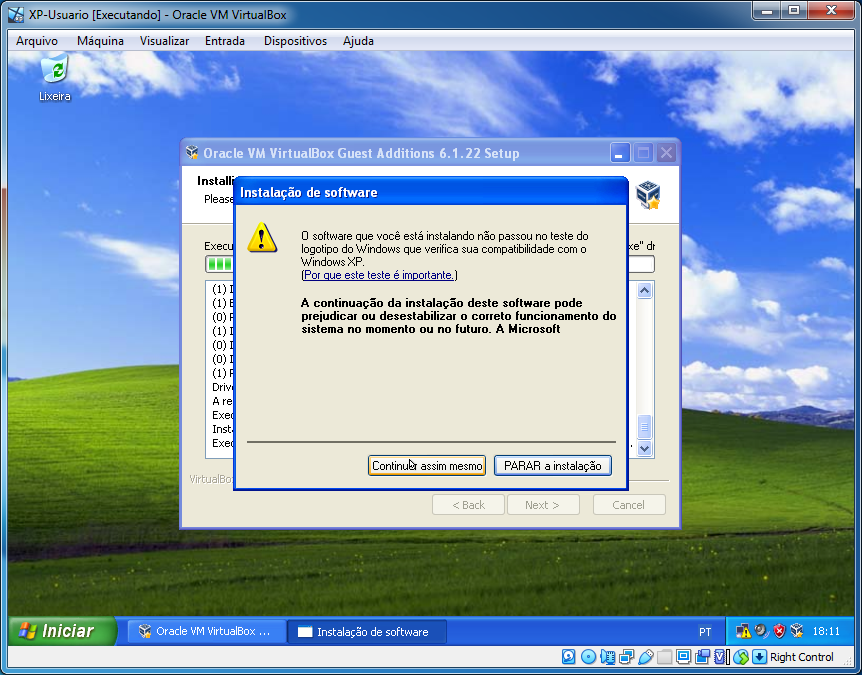
\includegraphics[width=\linewidth]{images/ativacao_das_maquinas_virtuais/configuracao_inicial_das_maquinas_virtuais/019.png}
\end{figure}
\begin{figure}[H]
    \centering
    \caption{Clique em \textbf{Continuar assim mesmo}}
    \label{fig:3120}
    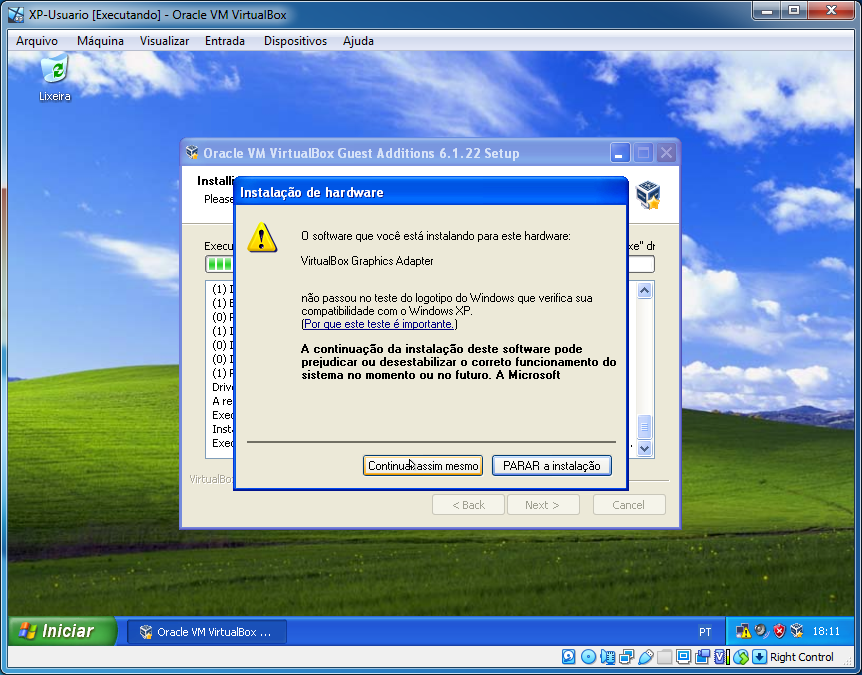
\includegraphics[width=\linewidth]{images/ativacao_das_maquinas_virtuais/configuracao_inicial_das_maquinas_virtuais/020.png}
\end{figure}
\begin{figure}[H]
    \centering
    \caption{Clique em \textbf{Continuar assim mesmo}}
    \label{fig:3121}
    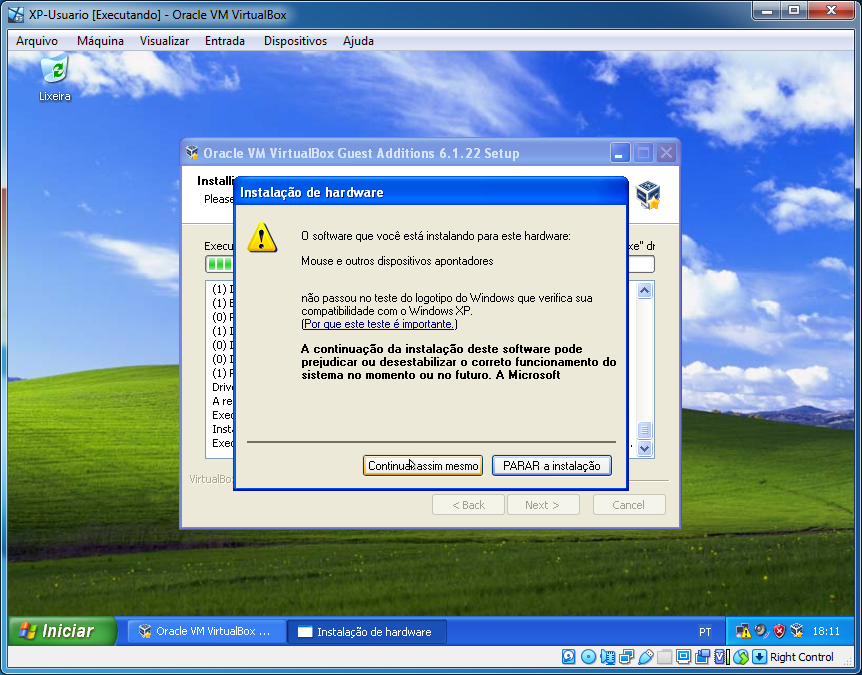
\includegraphics[width=\linewidth]{images/ativacao_das_maquinas_virtuais/configuracao_inicial_das_maquinas_virtuais/021.png}
\end{figure}
\begin{figure}[H]
    \centering
    \caption{Clique em \textbf{Finish}}
    \label{fig:3122}
    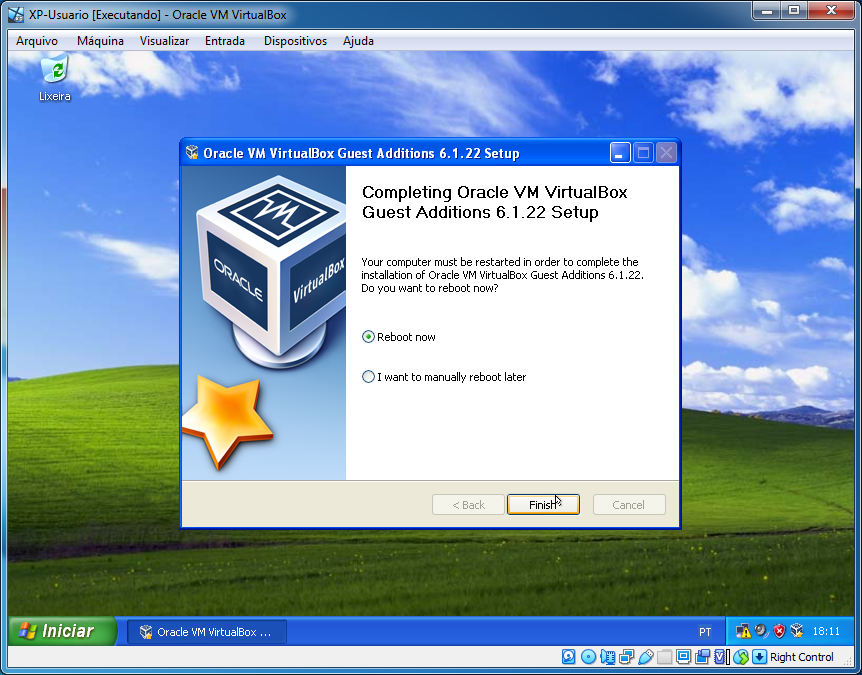
\includegraphics[width=\linewidth]{images/ativacao_das_maquinas_virtuais/configuracao_inicial_das_maquinas_virtuais/022.png}
\end{figure}
\begin{figure}[H]
    \centering
    \caption{Clique em \textbf{Iniciar}}
    \label{fig:3124}
    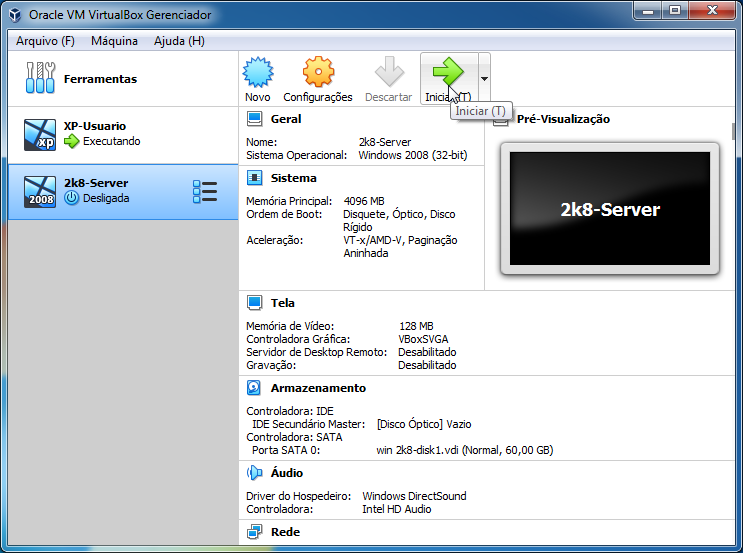
\includegraphics[width=\linewidth]{images/ativacao_das_maquinas_virtuais/configuracao_inicial_das_maquinas_virtuais/024.png}
\end{figure}
\begin{figure}[H]
    \centering
    \caption{Clique em \textbf{Iniciar o Windows Normalmente}}
    \label{fig:3125}
    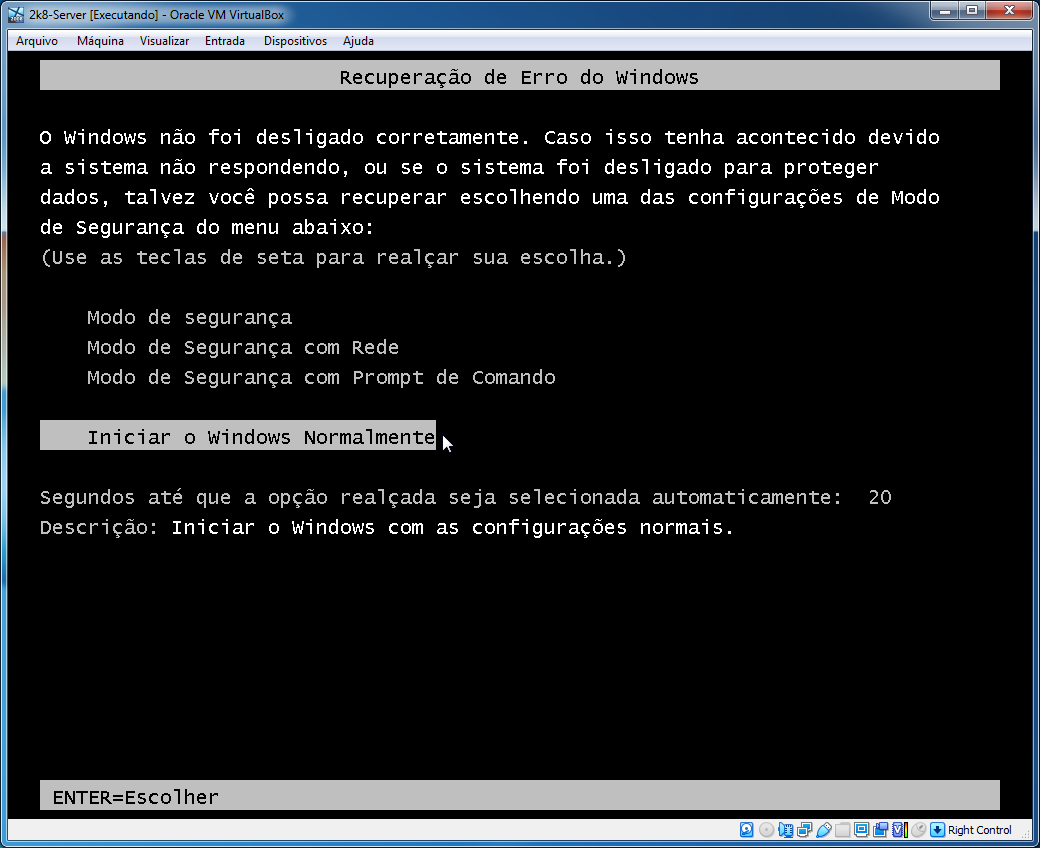
\includegraphics[width=\linewidth]{images/ativacao_das_maquinas_virtuais/configuracao_inicial_das_maquinas_virtuais/025.png}
\end{figure}
\begin{figure}[H]
    \centering
    \caption{Clique em \textbf{OK}}
    \label{fig:3126}
    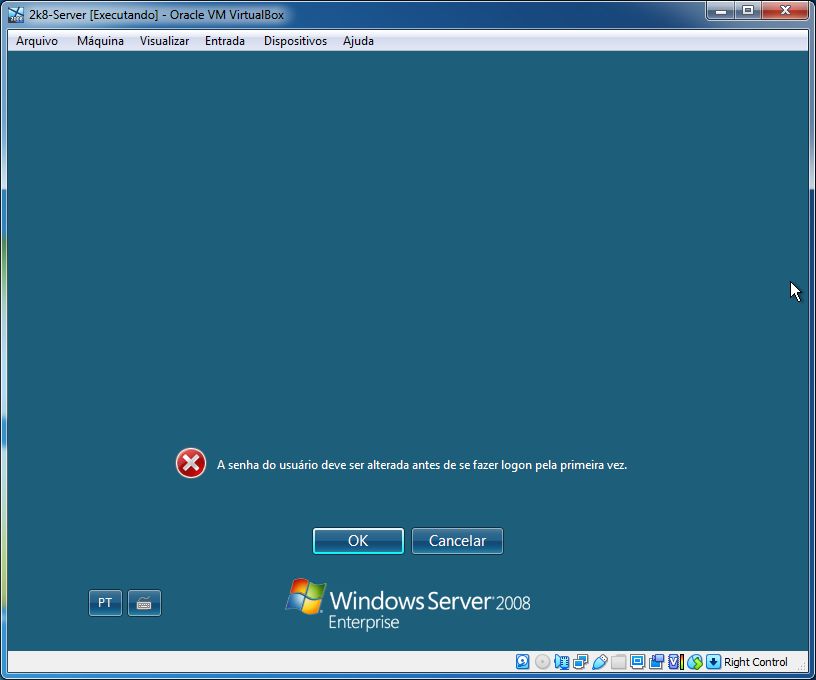
\includegraphics[width=\linewidth]{images/ativacao_das_maquinas_virtuais/configuracao_inicial_das_maquinas_virtuais/026.png}
\end{figure}
\begin{figure}[H]
    \centering
    \caption{Clique na seta ou de enter}
    \label{fig:3127}
    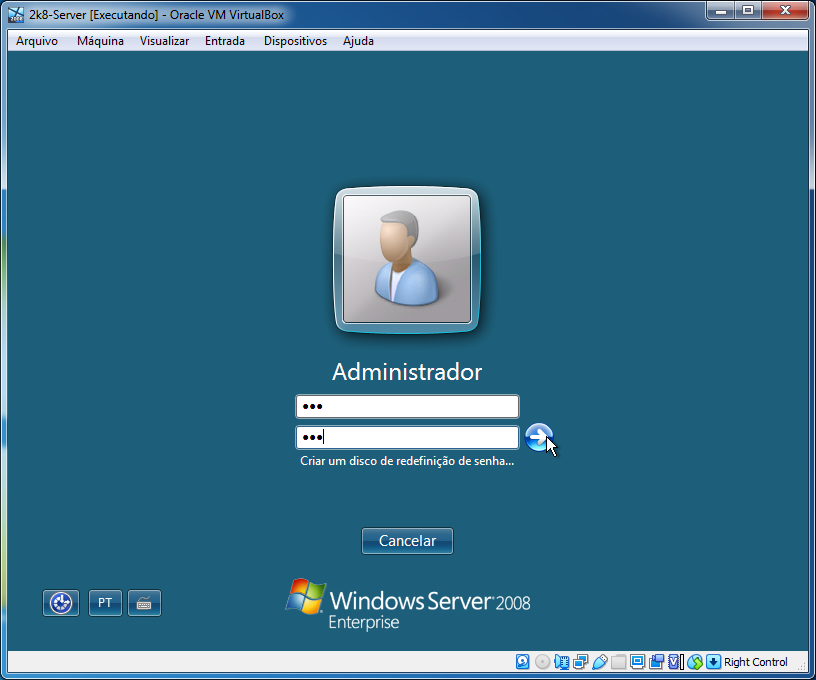
\includegraphics[width=\linewidth]{images/ativacao_das_maquinas_virtuais/configuracao_inicial_das_maquinas_virtuais/027.png}
\end{figure}
\begin{figure}[H]
    \centering
    \caption{Clique em \textbf{Ativar mais tarde} ou em \textbf{Cancelar}}
    \label{fig:3129}
    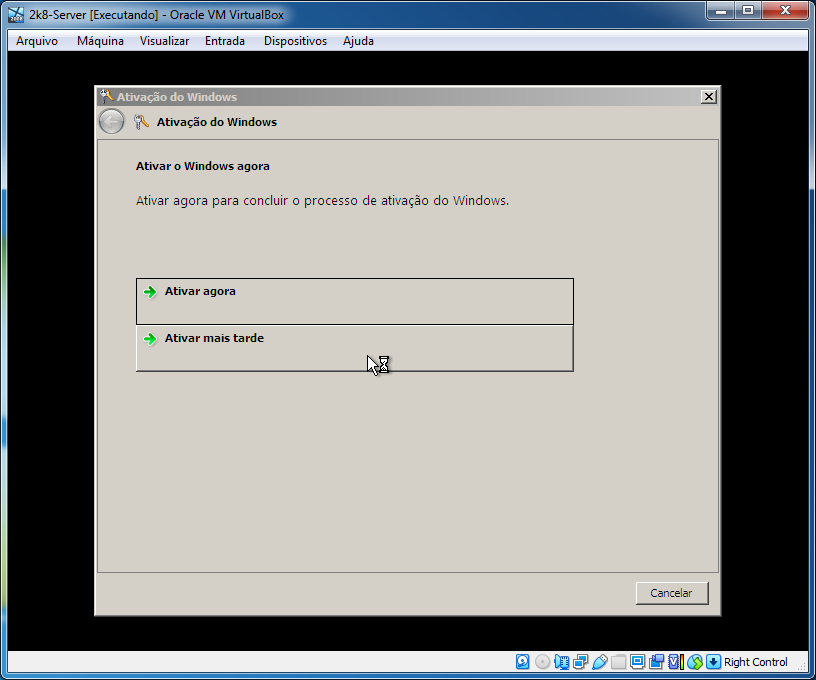
\includegraphics[width=\linewidth]{images/ativacao_das_maquinas_virtuais/configuracao_inicial_das_maquinas_virtuais/029.png}
\end{figure}
\begin{figure}[H]
    \centering
    \caption{Clique em \textbf{Dispositivos - Inserir imagem de CD dos Adicionais para Convidado}}
    \label{fig:3130}
    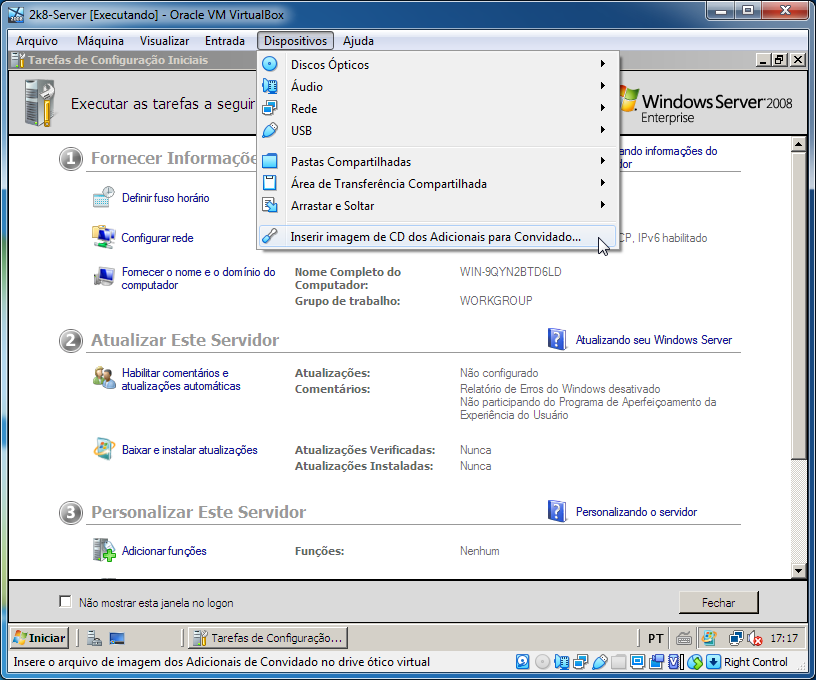
\includegraphics[width=\linewidth]{images/ativacao_das_maquinas_virtuais/configuracao_inicial_das_maquinas_virtuais/030.png}
\end{figure}
\begin{figure}[H]
    \centering
    \caption{Clique em \textbf{Executar VBoxWindowsAdditions.exe}}
    \label{fig:3131}
    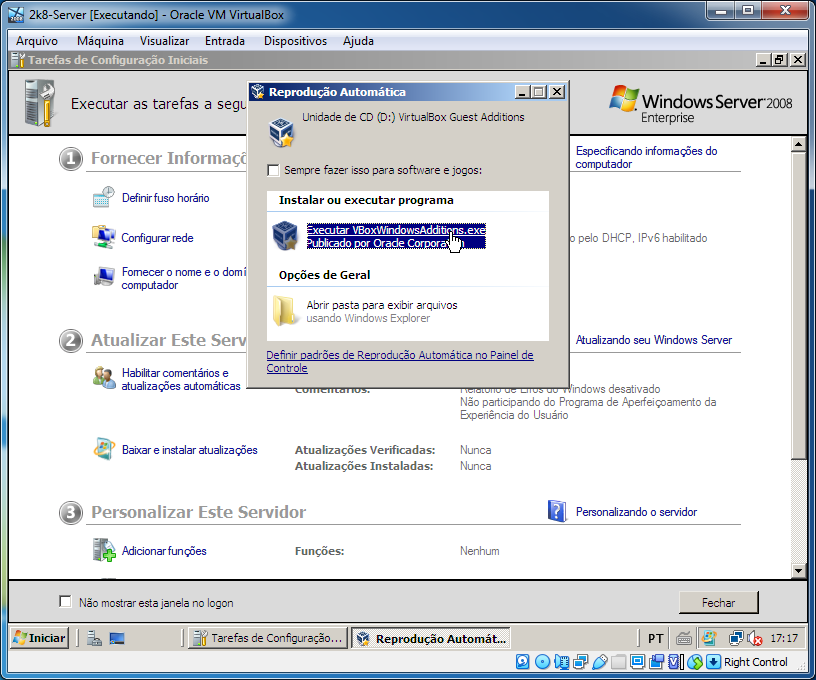
\includegraphics[width=\linewidth]{images/ativacao_das_maquinas_virtuais/configuracao_inicial_das_maquinas_virtuais/031.png}
\end{figure}
\begin{figure}[H]
    \centering
    \caption{Clique em \textbf{Next}}
    \label{fig:3132}
    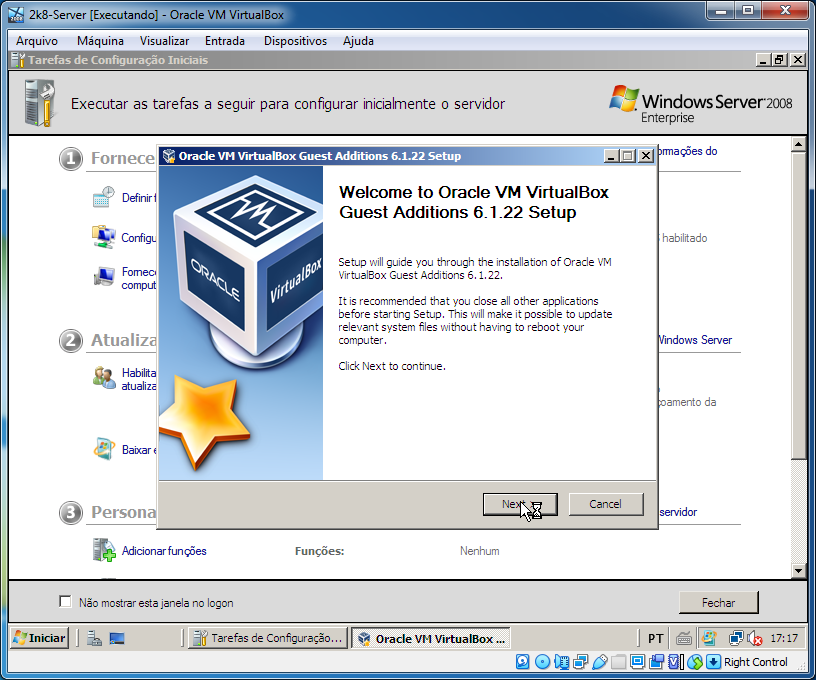
\includegraphics[width=\linewidth]{images/ativacao_das_maquinas_virtuais/configuracao_inicial_das_maquinas_virtuais/032.png}
\end{figure}
\begin{figure}[H]
    \centering
    \caption{Clique em \textbf{Next}}
    \label{fig:3133}
    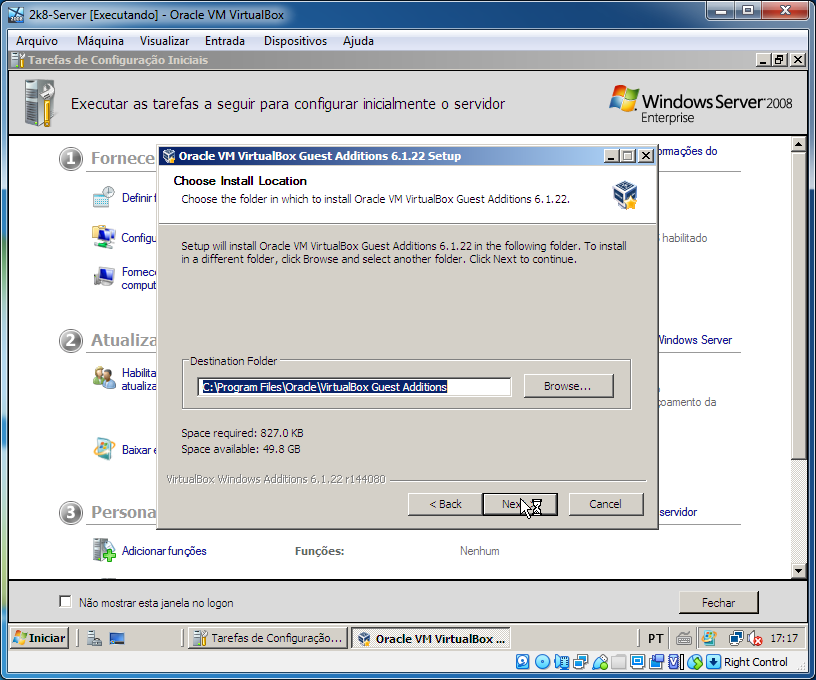
\includegraphics[width=\linewidth]{images/ativacao_das_maquinas_virtuais/configuracao_inicial_das_maquinas_virtuais/033.png}
\end{figure}
\begin{figure}[H]
    \centering
    \caption{Clique em \textbf{Install}}
    \label{fig:3134}
    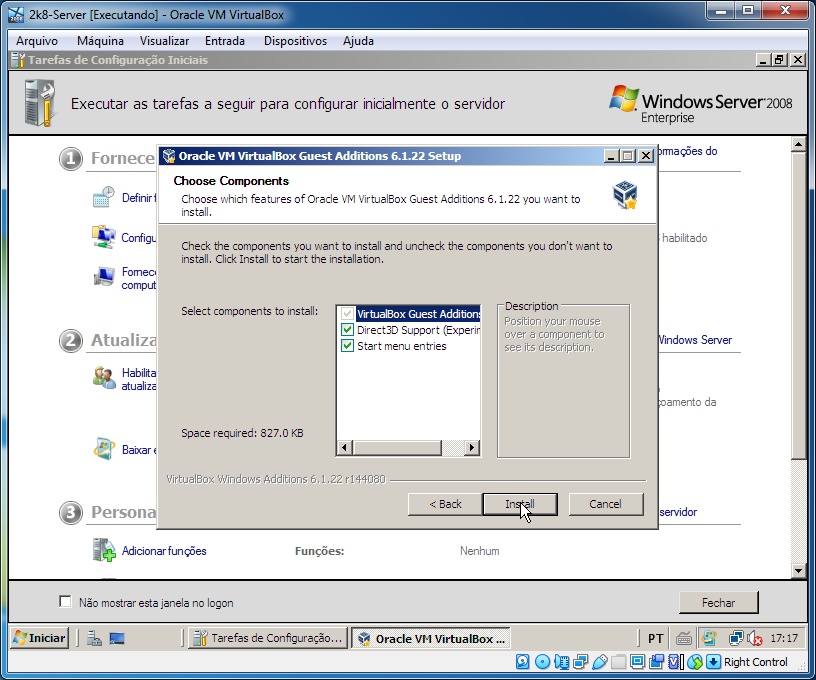
\includegraphics[width=\linewidth]{images/ativacao_das_maquinas_virtuais/configuracao_inicial_das_maquinas_virtuais/034.png}
\end{figure}
\begin{figure}[H]
    \centering
    \caption{Clique em \textbf{Instalar este software de driver mesmo assim}}
    \label{fig:3135}
    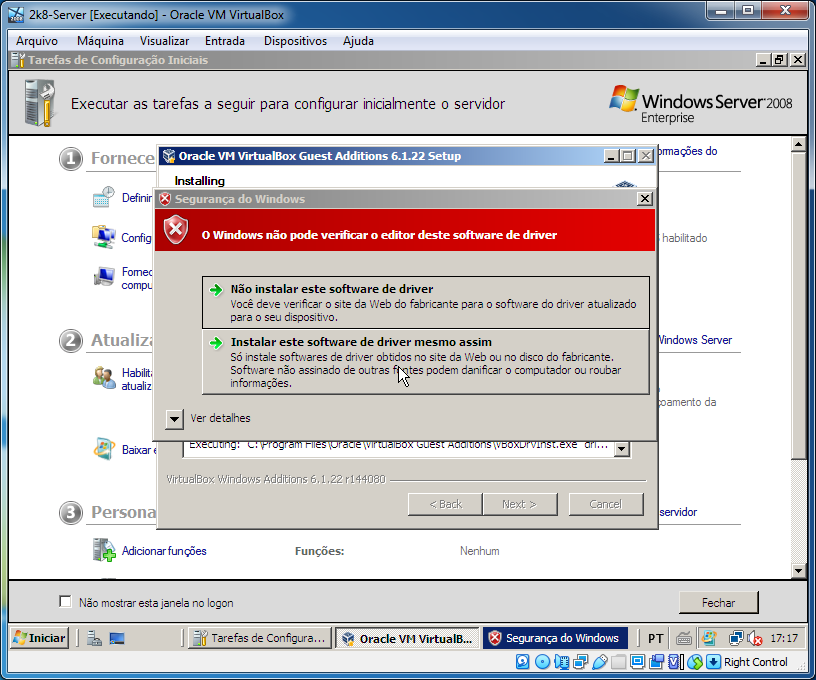
\includegraphics[width=\linewidth]{images/ativacao_das_maquinas_virtuais/configuracao_inicial_das_maquinas_virtuais/035.png}
\end{figure}
\begin{figure}[H]
    \centering
    \caption{Clique em \textbf{Instalar este software de driver mesmo assim}}
    \label{fig:3136}
    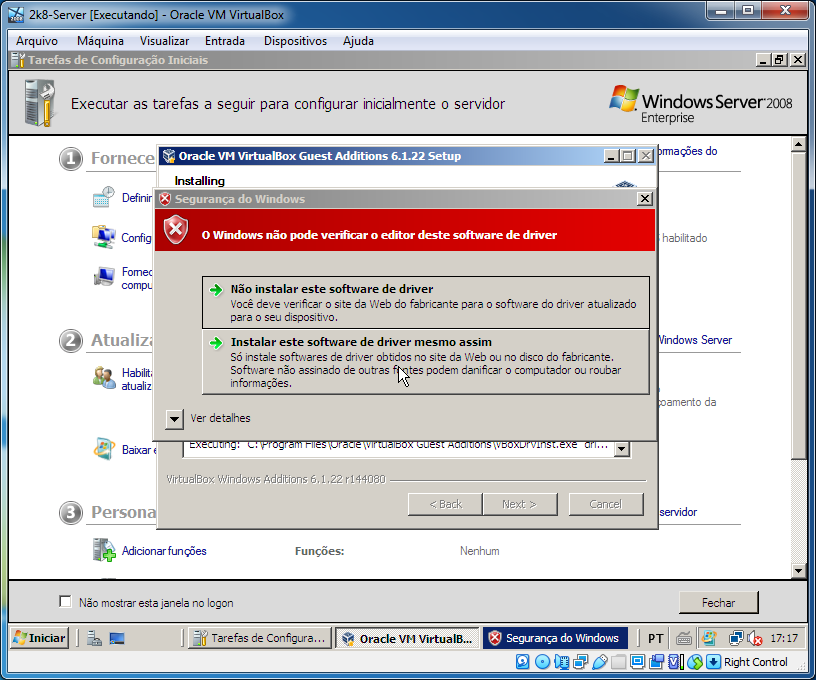
\includegraphics[width=\linewidth]{images/ativacao_das_maquinas_virtuais/configuracao_inicial_das_maquinas_virtuais/036.png}
\end{figure}
\begin{figure}[H]
    \centering
    \caption{Clique em \textbf{Cancel}}
    \label{fig:3137}
    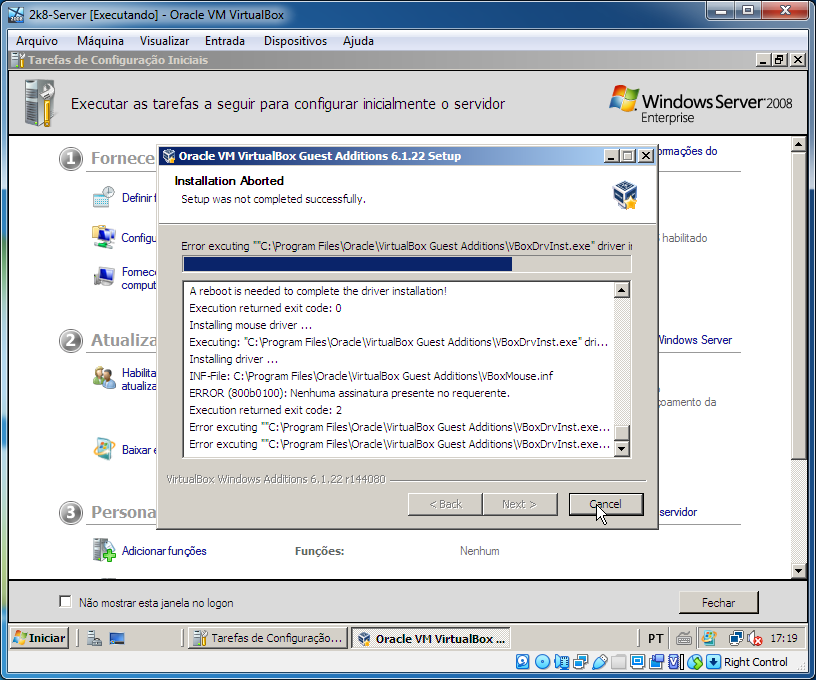
\includegraphics[width=\linewidth]{images/ativacao_das_maquinas_virtuais/configuracao_inicial_das_maquinas_virtuais/037.png}
\end{figure}
\begin{figure}[H]
    \centering
    \caption{Clique em \textbf{OK}}
    \label{fig:3138}
    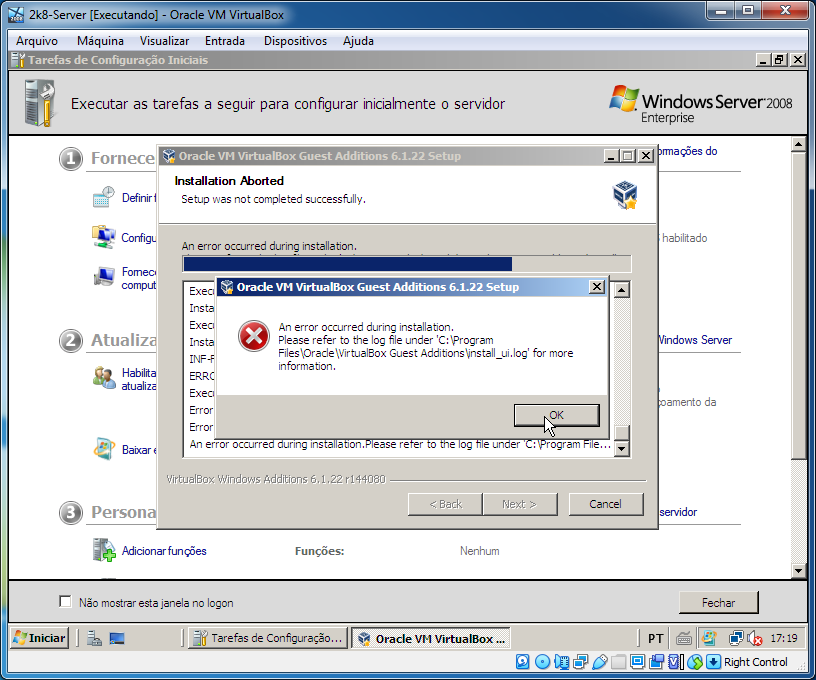
\includegraphics[width=\linewidth]{images/ativacao_das_maquinas_virtuais/configuracao_inicial_das_maquinas_virtuais/038.png}
\end{figure}
\begin{figure}[H]
    \centering
    \caption{Clique em \textbf{Reiniciar}}
    \label{fig:3139}
    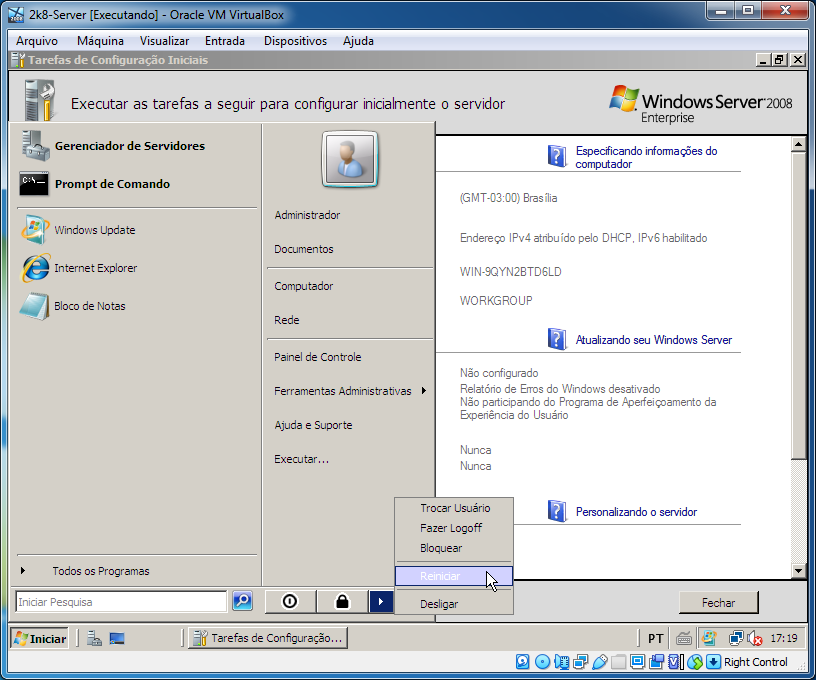
\includegraphics[width=\linewidth]{images/ativacao_das_maquinas_virtuais/configuracao_inicial_das_maquinas_virtuais/039.png}
\end{figure}
\begin{figure}[H]
    \centering
    \caption{Escreva algo na caixa de \textbf{Comentário:} e {Clique em \textbf{OK}}}
    \label{fig:3141}
    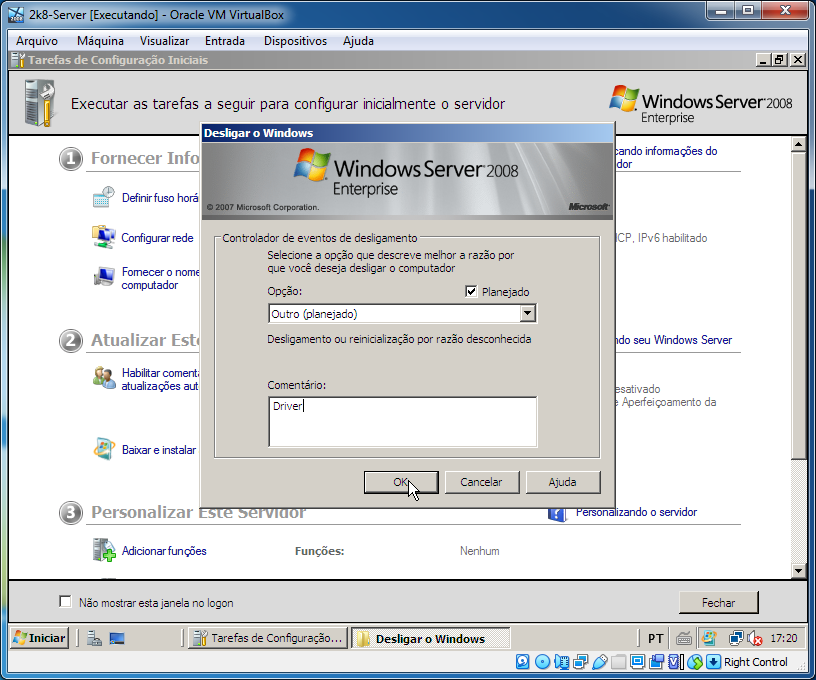
\includegraphics[width=\linewidth]{images/ativacao_das_maquinas_virtuais/configuracao_inicial_das_maquinas_virtuais/041.png}
\end{figure}
\begin{figure}[H]
    \centering
    \caption{Aperte CTRL(Direito) + DEL \textbf{Cancel}}
    \label{fig:3142}
    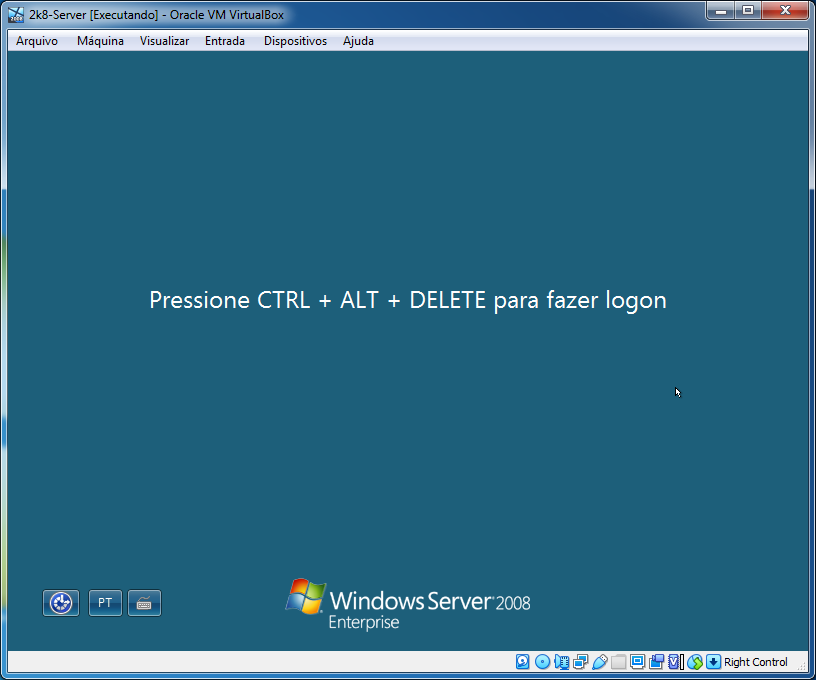
\includegraphics[width=\linewidth]{images/ativacao_das_maquinas_virtuais/configuracao_inicial_das_maquinas_virtuais/042.png}
\end{figure}
\begin{figure}[H]
    \centering
    \caption{Escreva a senha e de \textbf{enter}}
    \label{fig:3144}
    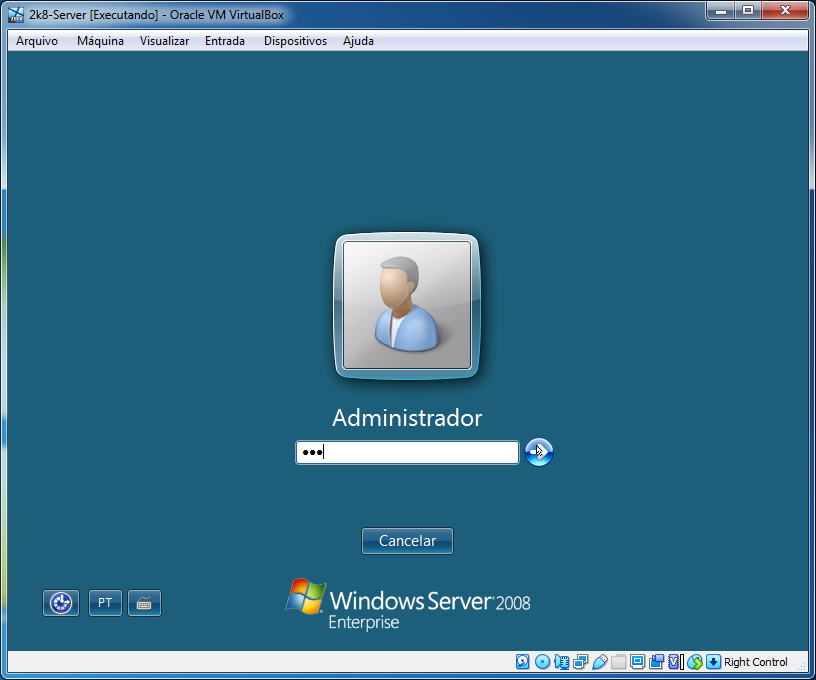
\includegraphics[width=\linewidth]{images/ativacao_das_maquinas_virtuais/configuracao_inicial_das_maquinas_virtuais/044.png}
\end{figure}
\begin{figure}[H]
    \centering
    \caption{Clique em \textbf{Ativar mais tarde} ou em \textbf{Cancelar}}
    \label{fig:3145}
    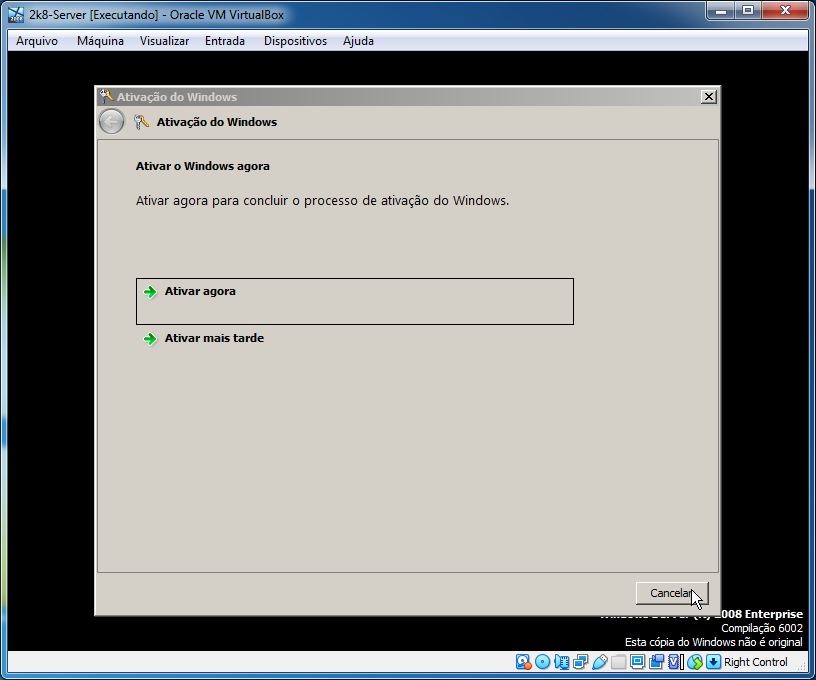
\includegraphics[width=\linewidth]{images/ativacao_das_maquinas_virtuais/configuracao_inicial_das_maquinas_virtuais/045.png}
\end{figure}
\begin{figure}[H]
    \centering
    \caption{Finalizado}
    \label{fig:3146}
    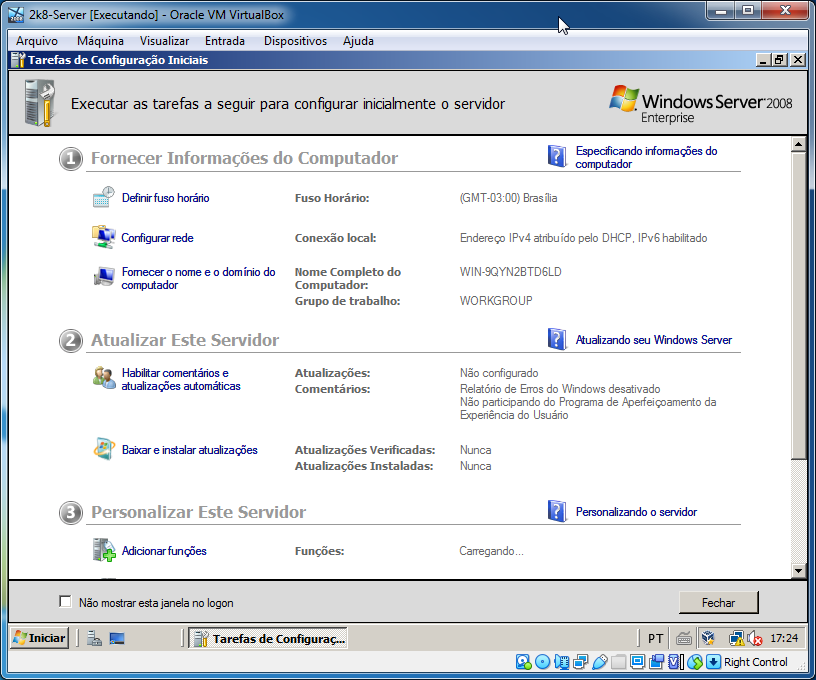
\includegraphics[width=\linewidth]{images/ativacao_das_maquinas_virtuais/configuracao_inicial_das_maquinas_virtuais/046.png}
\end{figure}


\section{CONFIGURAÇÃO DE REDE}
\subsection{Configuração Windows XP}
\subsubsection{Desabilitando o Firewall}
\par O Firewall do Windows pode ser desligado pelo Painel de Controle. Clique em \textbf{Iniciar} e depois em \textbf{Painel de Controle} (Figura \ref{fig:4111}). Depois clique em \textbf{Firewall do Windows} (Figura \ref{fig:4112}), em \textbf{Desativado} e em \textbf{OK} (Figura \ref{fig:4113}).

\begin{figure}[H]
    \centering
    \caption{Clique \textbf{Iniciar} e depois \textbf{Painel de Controle}.}
    \label{fig:4111}
    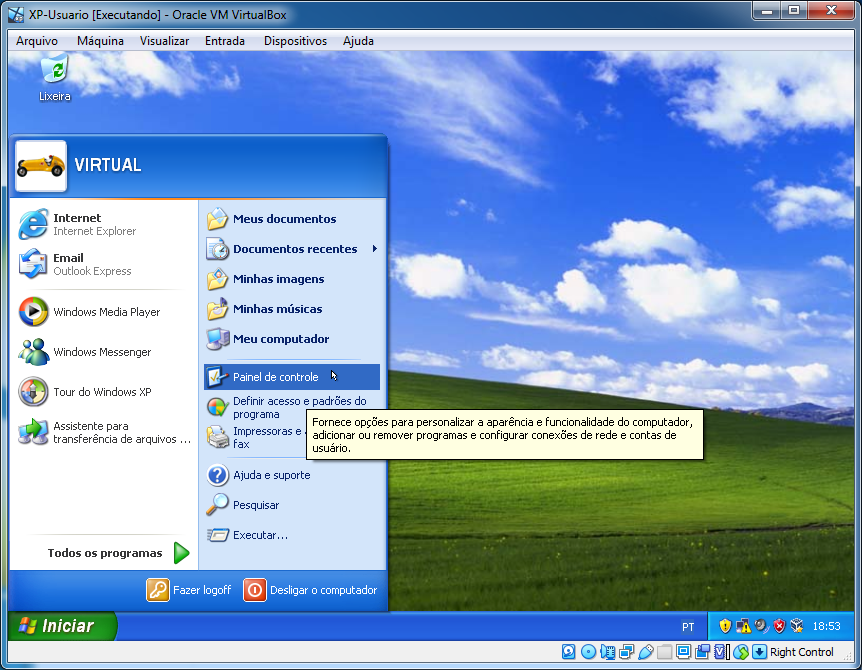
\includegraphics[width=\linewidth]{images/xp_rede/001.png}
\end{figure}

\begin{figure}[H]
    \centering
    \caption{Clique \textbf{Firewall do Windows}.}
    \label{fig:4112}
    \includegraphics[width=\linewidth]{images/xp_rede/002.png}
\end{figure}

\begin{figure}[H]
    \centering
    \caption{Clique \textbf{Desativado} e depois \textbf{OK}.}
    \label{fig:4113}
    \includegraphics[width=\linewidth]{images/xp_rede/003.png}
\end{figure}


\subsubsection{Configurando nome do computador e grupo de trabalho}
\par Acesse o Painel de Controle e clique em \textbf{Sistema} (Figura \ref{fig:4121}). Clique em \textbf{Alterar} (Figura \ref{fig:4122}). 
Mude o nome do computador para \textbf{usuario} (Figura \ref{fig:4123}). Digite \textbf{WORKGROUP} no grupo de trabalho e clique \textbf{OK} (Figura \ref{fig:4124}). A seguir, clique \textbf{OK} três vezes e \textbf{reinicie o computador} (Figura \ref{fig:4125}).

\begin{figure}[H]
    \centering
    \caption{Clique \textbf{Sistema}.}
    \label{fig:4121}
    \includegraphics[width=\linewidth]{images/xp_rede/004.png}
\end{figure}

\begin{figure}[H]
    \centering
    \caption{Clique \textbf{Alterar}.}
    \label{fig:4122}
    \includegraphics[width=\linewidth]{images/xp_rede/006.png}
\end{figure}

\begin{figure}[H]
    \centering
    \caption{Mude o nome do computador para \textbf{usuario}.}
    \label{fig:4123}
    \includegraphics[width=\linewidth]{images/xp_rede/007.png}
\end{figure}

\begin{figure}[H]
    \centering
    \caption{Digite \textbf{WORKGROUP} no grupo de trabalho e clique \textbf{OK}.}
    \label{fig:4124}
    \includegraphics[width=\linewidth]{images/xp_rede/008.png}
\end{figure}

\begin{figure}[H]
    \centering
    \caption{Clique \textbf{OK} três vezes e \textbf{reinicie o computador}.}
    \label{fig:4125}
    \includegraphics[width=\linewidth]{images/xp_rede/009.png}
\end{figure}

\subsubsection{Configurando o TCP/IP}
\par No Painel de Controle clique em \textbf{Conexões de rede} (Figura \ref{fig:4131}). A seguir, na janela de Conexões de rede, pressione com o botão direito na \textbf{Conexão Local} e selecione \textbf{Propriedades} (Figura \ref{fig:4132}). Nas Propriedades de Conexão Local, clique em \textbf{Protocolo TCP/IP} e clique em \textbf{Propriedades} (Figura \ref{fig:4133}). A seguir, preencha os seguintes dados (Figura \ref{fig:4134}): 
\begin{itemize}
    \item Endereço IP: 192.168.0.2
    \item Máscara de sub-rede: 255.255.255.0
    \item Gateway padrão: 192.168.0.1
    \item Servidor DNS preferencial: deixar em branco
    \item Servidor DNS alternativo: deixar em branco
\end{itemize}
\par Depois clique \textbf{OK}, \textbf{Fechar} e verifique se a conexão de rede está \textbf{conectada} (Figura \ref{fig:4135}).
\begin{figure}[H]
    \centering
    \caption{Clique \textbf{Conexões de rede}.}
    \label{fig:4131}
    \includegraphics[width=\linewidth]{images/xp_rede/013.png}
\end{figure}

\begin{figure}[H]
    \centering
    \caption{Selecione \textbf{Propriedades}.}
    \label{fig:4132}
    \includegraphics[width=\linewidth]{images/xp_rede/014.png}
\end{figure}

\begin{figure}[H]
    \centering
    \caption{Abra as \textbf{Propriedades} do \textbf{Protocolo TCP/IP}.}
    \label{fig:4133}
    \includegraphics[width=\linewidth]{images/xp_rede/015.png}
\end{figure}

\begin{figure}[H]
    \centering
    \caption{Preencha os campos do \textbf{endereço IP}.}
    \label{fig:4134}
    \includegraphics[width=\linewidth]{images/xp_rede/016.png}
\end{figure}

\begin{figure}[H]
    \centering
    \caption{Verifique se a conexão local está conectada.}
    \label{fig:4135}
    \includegraphics[width=\linewidth]{images/xp_rede/018.png}
\end{figure}


\subsection{Configuração Windows Server}
\subsubsection{Desabilitando o Firewall}
\par Agora, precisamos configurar o Windows Server, vamos começar desabilitando o \textbf{Firewall}. Para isso, vá no menu \textbf{Iniciar} e depois em \textbf{Painel de Controle} (Figura \ref{fig:4211}).
\par No Painel de Controle, dê dois cliques no \textbf{Firewall do Windows} (Figura \ref{fig:4212}). Provavelmente ele estará ativado, precisaremos desativar, para isso, clique em \textbf{Alterar configurações} (Figura \ref{fig:4213}).
\par Na janela que abriu, marque a opção \textbf{OFF} e clique em \textbf{OK} (Figura \ref{fig:4214}). Agora o Firewall está desativado (Figura \ref{fig:4215}), assim finalizamos a configuração do Firewall, pode fechar a janela.

\begin{figure}[H]
    \centering
    \caption{Acessando o Painel de Controle}
    \label{fig:4211}
    \includegraphics[width=\linewidth]{images/configuracao_windows/windows_server/001.png}
\end{figure}
\begin{figure}[H]
    \centering
    \caption{Painel de Controle}
    \label{fig:4212}
    \includegraphics[width=\linewidth]{images/configuracao_windows/windows_server/002.png}
\end{figure}
\begin{figure}[H]
    \centering
    \caption{Firewall do Windows}
    \label{fig:4213}
    \includegraphics[width=\linewidth]{images/configuracao_windows/windows_server/003.png}
\end{figure}
\begin{figure}[H]
    \centering
    \caption{Desativando o Firewall do Windows}
    \label{fig:4214}
    \includegraphics[width=\linewidth]{images/configuracao_windows/windows_server/005.png}
\end{figure}
\begin{figure}[H]
    \centering
    \caption{Firewall do Windows desativado}
    \label{fig:4215}
    \includegraphics[width=\linewidth]{images/configuracao_windows/windows_server/007.png}
\end{figure}


\subsubsection{Configurando nome do computador}
\par No \textbf{Painel de Controle}, dê dois cliques em \textbf{Sistema} (Figura \ref{fig:4221}). Assim que entrar na tela de \textbf{Sistema}, clique em \textbf{Alterar configurações} (Figura \ref{fig:4222}), em \textbf{Propriedades do Sistema}, clique no botão \textbf{Alterar} (Figura \ref{fig:4223}).
\par Na tela \textbf{Alterações de Nome/Domínio do Computador}, iremos alterar o \textbf{Nome do computador} para \textbf{server01}, após clique no botão \textbf{Mais...} (Figura \ref{fig:4224}), agora iremos configurar o \textbf{Sulfixo DNS} para \textbf{com} (Figura \ref{fig:4225}) e clique no botão \textbf{OK} e novamente clique no botão \textbf{OK}, com isso aparecerá uma janela informando que o sistema precisará ser reiniciado (Figura \ref{fig:4226}), clique em \textbf{OK}, depois \textbf{Fechar}, e por fim, \textbf{Reiniciar Agora} (Figura \ref{fig:4227}).
\begin{figure}[H]
    \centering
    \caption{Painel de Controle}
    \label{fig:4221}
    \includegraphics[width=\linewidth]{images/configuracao_windows/windows_server/008.png}
\end{figure}
\begin{figure}[H]
    \centering
    \caption{Alterar configurações do Sistema}
    \label{fig:4222}
    \includegraphics[width=\linewidth]{images/configuracao_windows/windows_server/009.png}
\end{figure}
\begin{figure}[H]
    \centering
    \caption{Alterar propriedades do Sistema}
    \label{fig:4223}
    \includegraphics[width=\linewidth]{images/configuracao_windows/windows_server/010.png}
\end{figure}
\begin{figure}[H]
    \centering
    \caption{Configurando nome do computador}
    \label{fig:4224}
    \includegraphics[width=\linewidth]{images/configuracao_windows/windows_server/011.png}
\end{figure}
\begin{figure}[H]
    \centering
    \caption{Configurando Sulfixo DNS}
    \label{fig:4225}
    \includegraphics[width=\linewidth]{images/configuracao_windows/windows_server/012.png}
\end{figure}
\begin{figure}[H]
    \centering
    \caption{Confirmando configurações}
    \label{fig:4226}
    \includegraphics[width=\linewidth]{images/configuracao_windows/windows_server/013.png}
\end{figure}
\begin{figure}[H]
    \centering
    \caption{Reiniciando sistema}
    \label{fig:4227}
    \includegraphics[width=\linewidth]{images/configuracao_windows/windows_server/015.png}
\end{figure}


\subsubsection{Configurando Centro de Rede e Compartilhamento}
\par Nessa sessão iremos configurar o \textbf{Compartilhamento e Descoberta} do servidor.
\par Acesse o \textbf{Painel de Controle}, em seguida dê dois cliques em \textbf{Centro de Rede e Compartilhamento} (Figura \ref{fig:4231}).
\par Em Compartilhamento e Descoberta, precisamos ativar \textbf{Descoberta de rede}, \textbf{Compartilhamento de arquivos} e \textbf{Compartilhamento de pasta pública}, para isso precisamos clicar na seta (Figura \ref{fig:4232}), escolher a opção \textbf{Ativar} e clique no botão \textbf{Aplicar} (Figura \ref{fig:4233}). 
\par Para ativar o \textbf{Compartilhamento de pasta pública}, precisamos escolher a opção \textbf{Ativar compartilhamento para que qualquer pessoa com acesso à rede possa abrir, alterar e criar arquivos} (Figura \ref{fig:4234}).
\par Em seguida desative o \textbf{Compartilhamento de impressora} e o \textbf{Compartilhamento protegido por senha} (Figura \ref{fig:4235}).
\par Com isso concluímos a configuração de descoberta e compartilhamento.

\begin{figure}[H]
    \centering
    \caption{Painel de Controle}
    \label{fig:4231}
    \includegraphics[width=\linewidth]{images/configuracao_windows/windows_server/021.png}
\end{figure}
\begin{figure}[H]
    \centering
    \caption{Centro de Rede e Compartilhamento}
    \label{fig:4232}
    \includegraphics[width=\linewidth]{images/configuracao_windows/windows_server/022.png}
\end{figure}
\begin{figure}[H]
    \centering
    \caption{Ativando descoberta de rede}
    \label{fig:4233}
    \includegraphics[width=\linewidth]{images/configuracao_windows/windows_server/024.png}
\end{figure}
\begin{figure}[H]
    \centering
    \caption{Ativando compartilhamento de pasta pública}
    \label{fig:4234}
    \includegraphics[width=\linewidth]{images/configuracao_windows/windows_server/028.png}
\end{figure}
\begin{figure}[H]
    \centering
    \caption{Compartilhamento e Descoberta configurados}
    \label{fig:4235}
    \includegraphics[width=\linewidth]{images/configuracao_windows/windows_server/030.png}
\end{figure}


\subsubsection{Configurando o TCP/IP}
\par No Painel de Controle clique em \textbf{Centro de Rede e Compartilhamento} (Figura \ref{fig:4241}), e após, clique em \textbf{Gerenciar conexão de rede} (Figura \ref{fig:4242}). A seguir, na janela \textbf{Conexões de Rede}, pressione com o botão direito na \textbf{Conexão Local} e selecione \textbf{Propriedades} (Figura \ref{fig:4243}). Nas Propriedades de Conexão Local, clique em \textbf{Protocolo TCP/IP Versão 4} e clique em \textbf{Propriedades} (Figura \ref{fig:4244}). A seguir, preencha os seguintes dados (Figura \ref{fig:4245}: 
\begin{itemize}
    \item Endereço IP: 192.168.0.1
    \item Máscara de sub-rede: 255.255.255.0
    \item Gateway padrão: 192.168.0.1
    \item Servidor DNS preferencial: deixar em branco
    \item Servidor DNS alternativo: deixar em branco
\end{itemize}
\par Depois clique \textbf{OK}, \textbf{Fechar} e verifique se a conexão de rede está \textbf{conectada} (Figura \ref{fig:4246}).
\begin{figure}[H]
    \centering
    \caption{Painel de Controle}
    \label{fig:4241}
    \includegraphics[width=\linewidth]{images/configuracao_windows/windows_server/021.png}
\end{figure}
\begin{figure}[H]
    \centering
    \caption{Centro de Rede e Compartilhamento}
    \label{fig:4242}
    \includegraphics[width=\linewidth]{images/configuracao_windows/windows_server/030.png}
\end{figure}
\begin{figure}[H]
    \centering
    \caption{}
    \label{fig:4243}
    \includegraphics[width=\linewidth]{images/configuracao_windows/windows_server/031.png}
\end{figure}
\begin{figure}[H]
    \centering
    \caption{}
    \label{fig:4244}
    \includegraphics[width=\linewidth]{images/configuracao_windows/windows_server/033.png}
\end{figure}
\begin{figure}[H]
    \centering
    \caption{}
    \label{fig:4245}
    \includegraphics[width=\linewidth]{images/configuracao_windows/windows_server/034.png}
\end{figure}
\begin{figure}[H]
    \centering
    \caption{}
    \label{fig:4246}
    \includegraphics[width=\linewidth]{images/configuracao_windows/windows_server/036.png}
\end{figure}
\subsection{Testando comunicação entre os Windows}
\par Para testar a comunicação entra os Windows é simples, estando no Windows XP basta ir em \textbf{Iniciar} e clicar em \textbf{Executar...} (Figura \ref{fig:443001}), agora digite \textbf{cmd} e de enter para abri o prompt de comando (Figura \ref{fig:443002}), com ele aberto escreva \textbf{ping 192.168.0.1} e de enter, fazendo isso confira se todos os Pacotes foram enviados e recebidos (Figura \ref{fig:443004}).
\par Agora faremos o mesmo porém no Windows Server, uma vez dentro do sistema vá em \textbf{Iniciar} escreva \textbf{cmd} e abra (Figura \ref{fig:443006}), com o prompt de comando aberto escreva \textbf{ping 192.168.0.2}, e novamente confira se todos os Pacotes foram enviados e recebidos (Figura \ref{fig:443008}).
\begin{figure}[H]
    \centering
    \caption{Em iniciar clique em \textbf{Executar...}}
    \label{fig:443001}
    \includegraphics[width=\linewidth]{images/xp_rede/testando_comunicação_entre_os_windows/001.png}
\end{figure}
\begin{figure}[H]
    \centering
    \caption{Escreva \textbf{cmd} e de enter}
    \label{fig:443002}
    \includegraphics[width=\linewidth]{images/xp_rede/testando_comunicação_entre_os_windows/002.png}
\end{figure}
\begin{figure}[H]
    \centering
    \caption{Digite \textbf{ping 192.168.0.1} e de enter}
    \label{fig:443004}
    \includegraphics[width=\linewidth]{images/xp_rede/testando_comunicação_entre_os_windows/004.png}
\end{figure}
\begin{figure}[H]
    \centering
    \caption{Em iniciar escreva \textbf{cmd} e abra}
    \label{fig:443006}
    \includegraphics[width=\linewidth]{images/xp_rede/testando_comunicação_entre_os_windows/006.png}
\end{figure}
\begin{figure}[H]
    \centering
    \caption{Digite \textbf{ping 192.168.0.2}}
    \label{fig:443008}
    \includegraphics[width=\linewidth]{images/xp_rede/testando_comunicação_entre_os_windows/008.png}
\end{figure}

\subsection{Compartilhamento de arquivos}
\par Nesta sessão, iremos aprender como compartilhar pastas e arquivos entre dois computadores na rede.
\subsubsection{Windows Server}
\par No \textbf{Windows Server}, na Área de Trabalho, crie uma pasta (Figura \ref{fig:5111}) com o nome que desejar, neste exemplo utilizaremos \textbf{Pasta-Server} (Figura \ref{fig:5112}). Agora iremos configurar o compartilhamento, basta clicar com o botão direito do mouse sobre a pasta criada e clique em \textbf{Propriedades} (Figura \ref{fig:5113}), em seguida clique em \textbf{Compartilhar} (Figura \ref{fig:5114}).
\par Na janela \textbf{Compartilhamento de Arquivos} que se abrir, clique na caixa de seleção e escolha a opção \textbf{Todos} (Figura \ref{fig:5115}), logo após clique em \textbf{Adicionar} (Figura \ref{fig:5116}). Após adicionado, você verá a opção que escolheu aparecer na lista abaixo da caixa de seleção, na coluna \textbf{Nível de Permissão}, mude o nível para \textbf{Parceria} (Figura \ref{fig:5117}) e clique em \textbf{Compartilhar}, será exibido como a pasta está compartilhada na rede, agora clique em \textbf{Pronto} (Figura \ref{fig:5118}).
\par Ainda na tela de propriedades da pasta, clique em \textbf{Compartilhamento Avançado} (Figura \ref{fig:5119}), marque a opção \textbf{Compartilhar a pasta} e após clique em \textbf{Permissões} (Figura \ref{fig:51110}). Marque a opção Controle total na coluna Permitir e clique em \textbf{OK} (Figura \ref{fig:51111}), após clique em \textbf{OK} novamente e \textbf{Fechar}.
\par Com isso terminamos de configurar o compartilhamento da pasta no Servidor, em seguida, vamos acessar a pasta pelo Windows XP.
\begin{figure}[H]
    \centering
    \caption{}
    \label{fig:5111}
    \includegraphics[width=\linewidth]{images/windows_server/compartilhamento/001.png}
\end{figure}
\begin{figure}[H]
    \centering
    \caption{}
    \label{fig:5112}
    \includegraphics[width=\linewidth]{images/windows_server/compartilhamento/002.png}
\end{figure}
\begin{figure}[H]
    \centering
    \caption{}
    \label{fig:5113}
    \includegraphics[width=\linewidth]{images/windows_server/compartilhamento/003.png}
\end{figure}
\begin{figure}[H]
    \centering
    \caption{}
    \label{fig:5114}
    \includegraphics[width=\linewidth]{images/windows_server/compartilhamento/005.png}
\end{figure}
\begin{figure}[H]
    \centering
    \caption{}
    \label{fig:5115}
    \includegraphics[width=\linewidth]{images/windows_server/compartilhamento/006.png}
\end{figure}
\begin{figure}[H]
    \centering
    \caption{}
    \label{fig:5116}
    \includegraphics[width=\linewidth]{images/windows_server/compartilhamento/007.png}
\end{figure}
\begin{figure}[H]
    \centering
    \caption{}
    \label{fig:5117}
    \includegraphics[width=\linewidth]{images/windows_server/compartilhamento/008.png}
\end{figure}
\begin{figure}[H]
    \centering
    \caption{}
    \label{fig:5118}
    \includegraphics[width=\linewidth]{images/windows_server/compartilhamento/010.png}
\end{figure}
\begin{figure}[H]
    \centering
    \caption{}
    \label{fig:5119}
    \includegraphics[width=\linewidth]{images/windows_server/compartilhamento/011.png}
\end{figure}
\begin{figure}[H]
    \centering
    \caption{}
    \label{fig:51110}
    \includegraphics[width=\linewidth]{images/windows_server/compartilhamento/013.png}
\end{figure}
\begin{figure}[H]
    \centering
    \caption{}
    \label{fig:51111}
    \includegraphics[width=\linewidth]{images/windows_server/compartilhamento/015.png}
\end{figure}
\subsubsection{Windows XP}
\par Após configurar a pasta compartilhana no Servidor, iremos acessar a pasta compartilhada no Windows XP.
\par Para isso, acesse o Windows XP, clique no menu Iniciar e clique em \textbf{Meu computador} (Figura \ref{fig:5121}). Na janela do Meu computador, clique no ícone das pastas ao lado da lupa para exibir a organização estruturada das pastas (Figura \ref{fig:5122}), após isso, clique em \textbf{Meus locais de rede} e com isso irá aparecer a pasta compartilhada, Pasta-Server no nosso exemplo (Figura \ref{fig:5123}), você pode expandir clicando no \textbf{+} do Meus locais de rede.
\par Agora iremos adicionar um atalho na Área de Trabalho para facilitar o acesso. Clique com o botão direito do mouse sobre a pasta compartilhada e clique em \textbf{Copiar} (Figura \ref{fig:5124}). Vá para a Área de Trabalho, clique com o botão direito do mouse, e clique na opção \textbf{Colar atalho} (Figura \ref{fig:5125}).
\par Agora vamos acessar a pasta e criar um arquivo de teste, dê dois cliques sobre o atalho criado na Área de Trabalho. Após abrir a pasta, crie um arquivo de texto dentro da pasta (Figura \ref{fig:5126}). Feito isso, vamos conferir se o arquivo aparece no Servidor, entre no Servidor e acesse a pasta que compartilhou, deve aparecer o arquivo de texto que criou pelo Windows XP (Figura \ref{fig:5127}).
\begin{figure}[H]
    \centering
    \caption{}
    \label{fig:5121}
    \includegraphics[width=\linewidth]{images/windows_server/compartilhamento/018.png}
\end{figure}
\begin{figure}[H]
    \centering
    \caption{}
    \label{fig:5122}
    \includegraphics[width=\linewidth]{images/windows_server/compartilhamento/020.png}
\end{figure}
\begin{figure}[H]
    \centering
    \caption{}
    \label{fig:5123}
    \includegraphics[width=\linewidth]{images/windows_server/compartilhamento/021.png}
\end{figure}
\begin{figure}[H]
    \centering
    \caption{}
    \label{fig:5124}
    \includegraphics[width=\linewidth]{images/windows_server/compartilhamento/023.png}
\end{figure}
\begin{figure}[H]
    \centering
    \caption{}
    \label{fig:5125}
    \includegraphics[width=\linewidth]{images/windows_server/compartilhamento/024.png}
\end{figure}
\begin{figure}[H]
    \centering
    \caption{}
    \label{fig:5126}
    \includegraphics[width=\linewidth]{images/windows_server/compartilhamento/026.png}
\end{figure}
\begin{figure}[H]
    \centering
    \caption{}
    \label{fig:5127}
    \includegraphics[width=\linewidth]{images/windows_server/compartilhamento/027.png}
\end{figure}

\subsection{Acesso Remoto}

\par Para configurar o acesso remoto será necessário criar uma conta de usuário no Windows Server, habilitar o acesso remoto no Windows Server e finalmente realizar o acesso remoto pelo Windows XP. 

\subsubsection{Criando uma conta de usuário}

\par No Painel de Controle do Windows Server clique em \textbf{Contas de Usuário} (Figura \ref{fig:ar002}), depois em \textbf{Gerenciar outra conta} (Figura \ref{fig:ar003}) e na tela seguinte \textbf{Criar uma nova conta} (Figura \ref{fig:ar004}).

\par Preencha o nome da conta que será criada, nesse exemplo demos o nome de \textbf{novo-usuario}. Também escolhemos criar uma conta do tipo \textbf{Administrador}, então é necessário ter muito cuidado sobre quem fará esse acesso remoto. Agora selecione \textbf{Criar conta} (Figura \ref{fig:ar005}).

\par Volte para a tela Gerenciar Contas e acesse o \textbf{novo-usuario} (Figura \ref{fig:ar006}). Clique \textbf{Criar uma senha} (Figura \ref{fig:ar007}). Preencha com as senhas que deseja utilizar e clique \textbf{Criar senha} (Figura \ref{fig:ar008}).

\begin{figure}[H]
    \centering
    \caption{Clique \textbf{Contas de Usuário}}
    \label{fig:ar002}
    \includegraphics[width=\linewidth]{images/acesso_remoto/ar002.png}
\end{figure}
\begin{figure}[H]
    \centering
    \caption{Clique \textbf{Gerenciar outra conta}}
    \label{fig:ar003}
    \includegraphics[width=\linewidth]{images/acesso_remoto/ar003.png}
\end{figure}
\begin{figure}[H]
    \centering
    \caption{Clique \textbf{Criar uma nova conta}}
    \label{fig:ar004}
    \includegraphics[width=\linewidth]{images/acesso_remoto/ar004.png}
\end{figure}
\begin{figure}[H]
    \centering
    \caption{Insira o \textbf{nome}, clique \textbf{Administrador} e clique \textbf{Criar conta}}
    \label{fig:ar005}
    \includegraphics[width=\linewidth]{images/acesso_remoto/ar005.png}
\end{figure}
\begin{figure}[H]
    \centering
    \caption{Clique duplo em \textbf{novo-usuario}}
    \label{fig:ar006}
    \includegraphics[width=\linewidth]{images/acesso_remoto/ar006.png}
\end{figure}
\begin{figure}[H]
    \centering
    \caption{Clique \textbf{Criar uma senha}}
    \label{fig:ar007}
    \includegraphics[width=\linewidth]{images/acesso_remoto/ar007.png}
\end{figure}
\begin{figure}[H]
    \centering
    \caption{Informe a senha desejada e clique \textbf{Criar senha}}
    \label{fig:ar008}
    \includegraphics[width=\linewidth]{images/acesso_remoto/ar008.png}
\end{figure}

\subsubsection{Habilitando o acesso remoto}
\par No Painel de Controle do Windows Server clique \textbf{Sistema} (Figura \ref{fig:ar011}) e selecione \textbf{Alterar configurações} (Figura \ref{fig:ar012}).
\par Na aba \textbf{Remoto} clique em \textbf{Permitir conexões de computadores que estejam executando qualquer versão da Área de Trabalho Remota (menos seguro)} (Figura \ref{fig:ar013}). Essa opcão menos segura é necessária porque estaremos utilizando versão diferentes do sistema operacional para realizar o acesso remoto. Clique em \textbf{OK} na mensagem que aparecerá (Figura \ref{fig:ar014}). 
\par Voltando à tela de Propriedades do Sistema, pressione \textbf{Selecionar Usuários} (Figura \ref{fig:ar015}) e depois \textbf{Adicionar...} (Figura \ref{fig:ar016}). Agora digite o nome da conta de usuário que criamos na seção anterior (\textbf{novo-usuario} no nosso exemplo) e clique \textbf{Verificar nomes} (Figura \ref{fig:ar017}). Se a conta de usuário for encontrada, ela será renomeada para algo similar a \textbf{SERVER01\textbackslash novo-usuario} (Figura \ref{fig:ar018}). Pronto, finalmente poderemos testar o acesso remoto. 

\begin{figure}[H]
    \centering
    \caption{Clique \textbf{Sistema}}
    \label{fig:ar011}
    \includegraphics[width=\linewidth]{images/acesso_remoto/ar011.png}
\end{figure}
\begin{figure}[H]
    \centering
    \caption{Clique \textbf{Alterar configurações}}
    \label{fig:ar012}
    \includegraphics[width=\linewidth]{images/acesso_remoto/ar012.png}
\end{figure}
\begin{figure}[H]
    \centering
    \caption{Na aba \textbf{Remoto} clique na \textbf{segunda opção}}
    \label{fig:ar013}
    \includegraphics[width=\linewidth]{images/acesso_remoto/ar013.png}
\end{figure}
\begin{figure}[H]
    \centering
    \caption{Clique \textbf{OK}}
    \label{fig:ar014}
    \includegraphics[width=\linewidth]{images/acesso_remoto/ar014.png}
\end{figure}
\begin{figure}[H]
    \centering
    \caption{Clique \textbf{Selecionar Usuários...}}
    \label{fig:ar015}
    \includegraphics[width=\linewidth]{images/acesso_remoto/ar015.png}
\end{figure}
\begin{figure}[H]
    \centering
    \caption{Clique \textbf{Adicionar}}
    \label{fig:ar016}
    \includegraphics[width=\linewidth]{images/acesso_remoto/ar016.png}
\end{figure}
\begin{figure}[H]
    \centering
    \caption{Escreva \textbf{novo-usuario} e selecione \textbf{Verificar nomes}}
    \label{fig:ar017}
    \includegraphics[width=\linewidth]{images/acesso_remoto/ar017.png}
\end{figure}
\begin{figure}[H]
    \centering
    \caption{A conta será renomeada para \textbf{SERVER01\textbackslash novo-usuario}}
    \label{fig:ar018}
    \includegraphics[width=\linewidth]{images/acesso_remoto/ar018.png}
\end{figure}
\begin{figure}[H]
    \centering
    \caption{Clique \textbf{OK}}
    \label{fig:ar019}
    \includegraphics[width=\linewidth]{images/acesso_remoto/ar019.png}
\end{figure}

\subsubsection{Realizando o acesso remoto}
\par No menu \textbf{Iniciar} do Windows XP selecione \textbf{Todos os programas}, \textbf{Acessórios} e clique em \textbf{Conexão de Área de Trabalho Remota} (Figura \ref{fig:ar021}). A seguir clique em \textbf{Opções >>} (Figura \ref{fig:ar022}). Preencha o IP do Windows Server \textbf{192.168.0.1}, o Nome de usuário \textbf{novo-usuario} e, se quiser, selecione \textbf{Permitir salvar minhas credenciais} (Figura \ref{fig:ar023}). Agora clique em \textbf{Conectar}. Insira a \textbf{senha} do novo-usuario e clique \textbf{OK} (Figura \ref{fig:ar024}). 
\par Acesso remoto realizado com sucesso \textbf{OK} (Figura \ref{fig:ar025}). Para sair clique no \textbf{X} da barra no topo da janela \textbf{OK} (Figura \ref{fig:ar027}) e depois \textbf{OK} (Figura \ref{fig:ar028}).

\begin{figure}[H]
    \centering
    \caption{Clique \textbf{Conexão de Área de Trabalho Remota}}
    \label{fig:ar021}
    \includegraphics[width=\linewidth]{images/acesso_remoto/ar021.png}
\end{figure}
\begin{figure}[H]
    \centering
    \caption{Clique em \textbf{Opções >>}}
    \label{fig:ar022}
    \includegraphics[width=\linewidth]{images/acesso_remoto/ar022.png}
\end{figure}
\begin{figure}[H]
    \centering
    \caption{Computador: \textbf{192.168.0.1}, Nome de usuário: \textbf{novo-usuario}.}
    \label{fig:ar023}
    \includegraphics[width=\linewidth]{images/acesso_remoto/ar023.png}
\end{figure}
\begin{figure}[H]
    \centering
    \caption{Insira a \textbf{senha} do novo-usuario e clique \textbf{OK}}
    \label{fig:ar024}
    \includegraphics[width=\linewidth]{images/acesso_remoto/ar024.png}
\end{figure}
\begin{figure}[H]
    \centering
    \caption{Acesso remoto realizado}
    \label{fig:ar025}
    \includegraphics[width=\linewidth]{images/acesso_remoto/ar025.png}
\end{figure}

\begin{figure}[H]
    \centering
    \caption{Para sair clique no \textbf{X} da barra no topo da janela}
    \label{fig:ar027}
    \includegraphics[width=\linewidth]{images/acesso_remoto/ar027.png}
\end{figure}
\begin{figure}[H]
    \centering
    \caption{Clique \textbf{OK}}
    \label{fig:ar028}
    \includegraphics[width=\linewidth]{images/acesso_remoto/ar028.png}
\end{figure}


\section{WINDOWS SERVER}

\subsection{Servidor DNS}
\par Pra começar vamos adiciontar a função \textbf{Servidor DNS} para isso abra o \textbf{Gerenciador de Servidores} clicando no ícone ao lado de iniciar (Figura \ref{fig:DNS001}), em funções clique em \textbf{Adicionar funções} (Figura \ref{fig:DNS003}), abrindo a janela de Assistente para Adicioanr Funções clique em \textbf{Próximo} (Figura \ref{fig:DNS004}), selecione \textbf{Servidor DNS} e clique em \textbf{Próximo} (Figura \ref{fig:DNS006}), clique em \textbf{Próximo} (Figura \ref{fig:DNS007}), clique em \textbf{Instalar} (Figura \ref{fig:DNS008}), após termianr a instalação cliqeu em \textbf{Fechar} (Figura \ref{fig:DNS010}). 
\par Agora para criar uma nova zona vá em \textbf{Iniciar, Ferramentas Administrativas, DNS} (Figura \ref{fig:DNS011}), dentro do Gerenciador DNS clique no \textbf{+} em \textbf{SERVER01}, clique com o botão direito na pasta \textbf{Zonas de pesquisa direta} e clique em \textbf{Nova zona...} (Figura \ref{fig:DNS013}), abrindo a janela de Assistente de nova zona clique em \textbf{Acançar} (Figura \ref{fig:DNS014}), deixe selecionado \textbf{Zona primária} e clique em \textbf{Acançar} (Figura \ref{fig:DNS015}), no campo de \textbf{Nome da zona:} escreva \textbf{server01.com} e de \textbf{Acançar} (Figura \ref{fig:DNS016}), no campo de \textbf{Criar um novo arquivo com este nome:} escreva \textbf{server01.com.dns} e de \textbf{Avançar} (Figura \ref{fig:DNS017}), deixe selecionado a opção \textbf{Não permitir atualizações dinâmicas} e de \textbf{Avançar} (Figura \ref{fig:DNS018}), após terminar volte no \textbf{Gerenciador DNS}, clique com o botão direito na pasta \textbf{Zonas de pesquisa inversa} e clique em \textbf{Nova zona...} (Figura \ref{fig:DNS020}), abrindo a janela de Assistente de nova zona clique em \textbf{Avançar} (Figura \ref{fig:DNS021}), deixe selecionado \textbf{Zona primária} e clique em \textbf{Acançar} (Figura \ref{fig:DNS022}), selecione \textbf{Zona de Pesquisa Inversa IPv4} e clique em \textbf{Avançar} (Figura \ref{fig:DNS023}), em \textbf{Identificação de rede:} escreva \textbf{192.168.0} e clique em \textbf{Avançar} (Figura \ref{fig:DNS024}), em \textbf{Criar um novo arquivo com este nome:} escreva \textbf{0.168.192.in-addr.arpa.dns} e clique em \textbf{Avançar} (Figura \ref{fig:DNS025}), deixe selecionado o campo \textbf{Não permitir atualizações dinâmicas} e clique em \textbf{Avançar} (Figura \ref{fig:DNS026}), clique em \textbf{Concluir} (Figura \ref{fig:DNS027}). 
\par Após isso vamos configurar o \textbf{server01.com}, ainda no Gerenciador DNS, vá em \textbf{SERVER01}, \textbf{Zonas de pesquisa direta} e abra a pasta \textbf{server01.com} (Figura \ref{fig:DNS028}), dentro da pasta clique com o botão direito e selecione \textbf{Novo Host (A ou AAAA)...} (Figura \ref{fig:DNS029}), abrindo uma janela, no campo \textbf{Endereço IP:} escreva \textbf{192.168.0.1} e clique em \textbf{Adicionar host} (Figura \ref{fig:DNS030}), clique em \textbf{OK} (Figura \ref{fig:DNS031}), clique em \textbf{Concluído} (Figura \ref{fig:DNS032}), voltando na pasta novamente \textbf{server01.com} clique com o botão direito e selecione \textbf{Novo alias (CNAME)...} (Figura \ref{fig:DNS033}), no campo \textbf{Nome do alias (usa domínio pai se deixado em branco):} escreva \textbf{www}, após isso na mesma janela clique em \textbf{Procurar...} (Figura \ref{fig:DNS034}), clicando duas vezes entre em \textbf{SERVER01} (Figura \ref{fig:DNS035}), entre em \textbf{Zonas de p...} (Figura \ref{fig:DNS036}), entre em \textbf{server01.com} (Figura \ref{fig:DNS037}), agora deixe selecionado o arquivo \textbf{(igual à pas...} e clique em \textbf{OK} (Figura \ref{fig:DNS038}), agora clique em \textbf{OK} (Figura \ref{fig:DNS039}), voltando novamente em Gerenciador DNS, clique com o botão direito em \textbf{SERVER01} e selecione \textbf{Iniciar nslookup} (Figura \ref{fig:DNS040}), abrindo o CMD digite \textbf{server01.com} e de enter, depois digite \textbf{www.server01.com} e de enter novamente (Figura \ref{fig:DNS042}).

\begin{figure}[H]
    \centering
    \caption{Clique no ícone \textbf{Gerenciador de Servidores}}
    \label{fig:DNS001}
    \includegraphics[width=\linewidth]{images/windows_server/dns/001.png}
\end{figure}
\begin{figure}[H]
    \centering
    \caption{Selecione \textbf{Funções} e \textbf{Adicionar funções}}
    \label{fig:DNS003}
    \includegraphics[width=\linewidth]{images/windows_server/dns/003.png}
\end{figure}
\begin{figure}[H]
    \centering
    \caption{Clique em \textbf{Próximo}}
    \label{fig:DNS004}
    \includegraphics[width=\linewidth]{images/windows_server/dns/004.png}
\end{figure}
\begin{figure}[H]
    \centering
    \caption{Selecione \textbf{Servidor DNS} e clique em \textbf{Próximo}}
    \label{fig:DNS006}
    \includegraphics[width=\linewidth]{images/windows_server/dns/006.png}
\end{figure}
\begin{figure}[H]
    \centering
    \caption{Clique em \textbf{Próximo}}
    \label{fig:DNS007}
    \includegraphics[width=\linewidth]{images/windows_server/dns/007.png}
\end{figure}
\begin{figure}[H]
    \centering
    \caption{Clique em \textbf{Instalar}}
    \label{fig:DNS008}
    \includegraphics[width=\linewidth]{images/windows_server/dns/008.png}
\end{figure}
\begin{figure}[H]
    \centering
    \caption{Clique em \textbf{Fechar}}
    \label{fig:DNS010}
    \includegraphics[width=\linewidth]{images/windows_server/dns/010.png}
\end{figure}
\begin{figure}[H]
    \centering
    \caption{Clique em \textbf{Iniciar}, \textbf{Ferramentas Administrativas}, \textbf{DNS}}
    \label{fig:DNS011}
    \includegraphics[width=\linewidth]{images/windows_server/dns/011.png}
\end{figure}
\begin{figure}[H]
    \centering
    \caption{Clique no \textbf{+} em \textbf{SERVER01}}
    \label{fig:DNS012}
    \includegraphics[width=\linewidth]{images/windows_server/dns/012.png}
\end{figure}
\begin{figure}[H]
    \centering
    \caption{Botão direito na pasta \textbf{Zonas de pesquisa direta} e selecionar \textbf{Nova zona...}}
    \label{fig:DNS013}
    \includegraphics[width=\linewidth]{images/windows_server/dns/013.png}
\end{figure}
\begin{figure}[H]
    \centering
    \caption{Clique em \textbf{Avançar}}
    \label{fig:DNS014}
    \includegraphics[width=\linewidth]{images/windows_server/dns/014.png}
\end{figure}
\begin{figure}[H]
    \centering
    \caption{\textbf{Zona primário} e clique em \textbf{Avançar}}
    \label{fig:DNS015}
    \includegraphics[width=\linewidth]{images/windows_server/dns/015.png}
\end{figure}
\begin{figure}[H]
    \centering
    \caption{Nome da zona: \textbf{server01.com} e clique em \textbf{Avançar}}
    \label{fig:DNS016}
    \includegraphics[width=\linewidth]{images/windows_server/dns/016.png}
\end{figure}
\begin{figure}[H]
    \centering
    \caption{Criar um novo arquivo com este nome: \textbf{server01.com.dns} e clique em \textbf{Avançar}}
    \label{fig:DNS017}
    \includegraphics[width=\linewidth]{images/windows_server/dns/017.png}
\end{figure}
\begin{figure}[H]
    \centering
    \caption{\textbf{Não permitir atualizações dinâmicas} e clique em \textbf{Avançar}}
    \label{fig:DNS018}
    \includegraphics[width=\linewidth]{images/windows_server/dns/018.png}
\end{figure}
\begin{figure}[H]
    \centering
    \caption{Botão direito na pasta \textbf{Zonas de pesquisa inversa} e selecionar \textbf{Nova zona...}}
    \label{fig:DNS020}
    \includegraphics[width=\linewidth]{images/windows_server/dns/020.png}
\end{figure}
\begin{figure}[H]
    \centering
    \caption{Clique em \textbf{Avançar}}
    \label{fig:DNS021}
    \includegraphics[width=\linewidth]{images/windows_server/dns/021.png}
\end{figure}
\begin{figure}[H]
    \centering
    \caption{\textbf{Zona primário} e clique em \textbf{Avançar}}
    \label{fig:DNS022}
    \includegraphics[width=\linewidth]{images/windows_server/dns/022.png}
\end{figure}
\begin{figure}[H]
    \centering
    \caption{\textbf{Zona de Pesquisa Inversa IPv4} e clique em \textbf{Avançar}}
    \label{fig:DNS023}
    \includegraphics[width=\linewidth]{images/windows_server/dns/023.png}
\end{figure}
\begin{figure}[H]
    \centering
    \caption{Identificação de rede: \textbf{192.168.0} e clique em \textbf{Avançar}}
    \label{fig:DNS024}
    \includegraphics[width=\linewidth]{images/windows_server/dns/024.png}
\end{figure}
\begin{figure}[H]
    \centering
    \caption{Criar um novo arquivo com este nome: \textbf{0.168.192.in-addr.arpa.dns} e clique em \textbf{Avançar}}
    \label{fig:DNS025}
    \includegraphics[width=\linewidth]{images/windows_server/dns/025.png}
\end{figure}
\begin{figure}[H]
    \centering
    \caption{\textbf{Não permitir atualizações dinâmicas} e clique em \textbf{Avançar}}
    \label{fig:DNS026}
    \includegraphics[width=\linewidth]{images/windows_server/dns/026.png}
\end{figure}
\begin{figure}[H]
    \centering
    \caption{Clique em \textbf{Concluir}}
    \label{fig:DNS027}
    \includegraphics[width=\linewidth]{images/windows_server/dns/027.png}
\end{figure}
\begin{figure}[H]
    \centering
    \caption{Abrir a pasta \textbf{server01.com}}
    \label{fig:DNS028}
    \includegraphics[width=\linewidth]{images/windows_server/dns/028.png}
\end{figure}
\begin{figure}[H]
    \centering
    \caption{Botão direito e \textbf{Novo Host (A ou AAAA)...}}
    \label{fig:DNS029}
    \includegraphics[width=\linewidth]{images/windows_server/dns/029.png}
\end{figure}
\begin{figure}[H]
    \centering
    \caption{Endereço IP: \textbf{192.168.0.1} e clique em \textbf{Adicionar host}}
    \label{fig:DNS030}
    \includegraphics[width=\linewidth]{images/windows_server/dns/030.png}
\end{figure}
\begin{figure}[H]
    \centering
    \caption{Clique em \textbf{OK}}
    \label{fig:DNS031}
    \includegraphics[width=\linewidth]{images/windows_server/dns/031.png}
\end{figure}
\begin{figure}[H]
    \centering
    \caption{Clique em \textbf{Concluído}}
    \label{fig:DNS032}
    \includegraphics[width=\linewidth]{images/windows_server/dns/032.png}
\end{figure}
\begin{figure}[H]
    \centering
    \caption{Botão direito e \textbf{Novo alias (CNAME)...}}
    \label{fig:DNS033}
    \includegraphics[width=\linewidth]{images/windows_server/dns/033.png}
\end{figure}
\begin{figure}[H]
    \centering
    \caption{Em \textbf{Nome do alias:} escreva \textbf{www} e clique em \textbf{Procurar...}}
    \label{fig:DNS034}
    \includegraphics[width=\linewidth]{images/windows_server/dns/034.png}
\end{figure}
\begin{figure}[H]
    \centering
    \caption{Entre em \textbf{SERVER01}}
    \label{fig:DNS035}
    \includegraphics[width=\linewidth]{images/windows_server/dns/035.png}
\end{figure}
\begin{figure}[H]
    \centering
    \caption{Entre em \textbf{Zonas de p...}}
    \label{fig:DNS036}
    \includegraphics[width=\linewidth]{images/windows_server/dns/036.png}
\end{figure}
\begin{figure}[H]
    \centering
    \caption{Entre em \textbf{server01.com}}
    \label{fig:DNS037}
    \includegraphics[width=\linewidth]{images/windows_server/dns/037.png}
\end{figure}
\begin{figure}[H]
    \centering
    \caption{Selecione \textbf{(igual à pas...} e clique em \textbf{OK}}
    \label{fig:DNS038}
    \includegraphics[width=\linewidth]{images/windows_server/dns/038.png}
\end{figure}
\begin{figure}[H]
    \centering
    \caption{Clique em \textbf{OK}}
    \label{fig:DNS039}
    \includegraphics[width=\linewidth]{images/windows_server/dns/039.png}
\end{figure}
\begin{figure}[H]
    \centering
    \caption{Botão direito em \textbf{SERVER01} e clique em \textbf{Iniciar nslookup}}
    \label{fig:DNS040}
    \includegraphics[width=\linewidth]{images/windows_server/dns/040.png}
\end{figure}
\begin{figure}[H]
    \centering
    \caption{Digite \textbf{server01.com} e de enter, depois digite \textbf{www.server01.com} e de enter}
    \label{fig:DNS042}
    \includegraphics[width=\linewidth]{images/windows_server/dns/042.png}
\end{figure}

\subsection{DHCP}
\par Nesta sessão faremos a instalação e configuração do Servidor DHCP e após concliur iremos configurar o Windows XP para receber o IP automaticamente.
\subsubsection{Windows Server}
\par No servidor precisamos acessar o \textbf{Gerenciador de Servidores}, clicando no ícone ao lado do menu Iniciar, na janela que se abrir, clique na opção \textbf{Adicionar funções} (Figura \ref{fig:5311}), na janela do \textbf{Assistente para Adicionar Funções} clique em Próximo, na próxima tela maque a opção \textbf{Servidor DHCP} e clique em \textbf{Próximo} (Figura \ref{fig:5312}), clique em Próximo até chegar na tela de \textbf{Configurações de Servidor DNS IPv4}, nesta tela iremos configurar o Domínio Pai para \textbf{server01.com} e informe o endereço de IP \textbf{192.168.0.1} e clique em \textbf{Validar} (Figura \ref{fig:5313}). Assim que aparecer \textbf{Válido}, podemos avançar clicando em \textbf{Próximo}.
\par Na tela Configuraçnoes de Servidor IPv4 WINS, marque a opção \textbf{WINS não é necessário aos aplicativos desta rede}, após clique em \textbf{Próximo} (Figura \ref{fig:5314}).
\par Em Escopos DHCP, vamos adicionar o intervalo de IPs, clique em \textbf{Adicionar} (Figura \ref{fig:5315}), em seguida configure da seguinte forma:
\begin{itemize}
    \item Nome do Escopo: geral
    \item Endereço IP Inicial: 192.168.0.51
    \item Endereço IP Final: 192.168.0.250
    \item Máscara de sub-rede: 255.255.255.0
    \item Gateway padrão: 192.168.0.1
    \item Tipo de Sub-rede: Com fio
    \item Ativar este escopo: Marcado
\end{itemize}
\par Após configurar, clique em OK (Figura \ref{fig:5316}) e podemos avançar clicando em \textbf{Próximo}.
\par Em Modo Sem Monitoração de Estado do DHCPv6, deixe \textbf{Desativado} e pode avançar clicando em \textbf{Próximo}  (Figura \ref{fig:5317}).
\par Por fim, irá aparecer uma tela de confirmação com o resumo de todas as configurações executadas até o momento, basta clicar em \textbf{Instalar} e depois \textbf{Fechar} (Figura \ref{fig:5318})

\begin{figure}[H]
    \centering
    \caption{}
    \label{fig:5311}
    \includegraphics[width=\linewidth]{images/windows_server/dhcp/001.png}
\end{figure}
\begin{figure}[H]
    \centering
    \caption{}
    \label{fig:5312}
    \includegraphics[width=\linewidth]{images/windows_server/dhcp/004.png}
\end{figure}
\begin{figure}[H]
    \centering
    \caption{}
    \label{fig:5313}
    \includegraphics[width=\linewidth]{images/windows_server/dhcp/009.png}
\end{figure}
\begin{figure}[H]
    \centering
    \caption{}
    \label{fig:5314}
    \includegraphics[width=\linewidth]{images/windows_server/dhcp/010.png}
\end{figure}
\begin{figure}[H]
    \centering
    \caption{}
    \label{fig:5315}
    \includegraphics[width=\linewidth]{images/windows_server/dhcp/011.png}
\end{figure}
\begin{figure}[H]
    \centering
    \caption{}
    \label{fig:5316}
    \includegraphics[width=\linewidth]{images/windows_server/dhcp/012.png}
\end{figure}
\begin{figure}[H]
    \centering
    \caption{}
    \label{fig:5317}
    \includegraphics[width=\linewidth]{images/windows_server/dhcp/014.png}
\end{figure}
\begin{figure}[H]
    \centering
    \caption{}
    \label{fig:5318}
    \includegraphics[width=\linewidth]{images/windows_server/dhcp/015.png}
\end{figure}
\subsubsection{Windows XP}
\par Agora que configuramos o servidor de DHCP, podemos configurar o Windows XP para fazer uso desse serviço, para isso vamos acessar o Painel de Controle, e dar dois cliques sobre \textbf{Conexões de rede}  (Figura \ref{fig:5321}), em seguida, clicar com o botão direito do mouse sobre Conexão local e escolher a opção \textbf{Propriedades}  (Figura \ref{fig:5322}), escolha a opção Protocolo TCP/IP e clique em \textbf{Propriedades} (Figura \ref{fig:5323}).
\par Na janela de Propriedades de Protocolo TCP/IP, precisamos marcar as opções \textbf{Obter um endereço IP automaticamente} e \textbf{Obter o endereço dos servidores DNS automaticamente} e clicar em \textbf{OK} e OK novamente (Figura \ref{fig:5324}).
\par Agora para verificar que tudo ocorreu corretamente, podemos fazer um teste de PING, para isso, vá no menu Iniciar, e depois Prompt de comando (Figura \ref{fig:5325}), caso não tenha essa opção no menu Iniciar, você pode acessar menu Iniciar, e depois Executar, digite \textbf{cmd} e aperte ENTER.
\par Na janela do Prompt de comando, digite \textbf{ipconfig} e aperte ENTER, deve exibir o endereço de IP dentro do intervalo configurado no Servidor DHCP, no nosso exemplo exibirá \textbf{192.168.0.51} (Figura \ref{fig:5326}), e pronto, o Windows XP já está recebendo o IP automaticamente.
\begin{figure}[H]
    \centering
    \caption{}
    \label{fig:5321}
    \includegraphics[width=\linewidth]{images/windows_server/dhcp/019.png}
\end{figure}
\begin{figure}[H]
    \centering
    \caption{}
    \label{fig:5322}
    \includegraphics[width=\linewidth]{images/windows_server/dhcp/020.png}
\end{figure}
\begin{figure}[H]
    \centering
    \caption{}
    \label{fig:5323}
    \includegraphics[width=\linewidth]{images/windows_server/dhcp/022.png}
\end{figure}
\begin{figure}[H]
    \centering
    \caption{}
    \label{fig:5324}
    \includegraphics[width=\linewidth]{images/windows_server/dhcp/024.png}
\end{figure}
\begin{figure}[H]
    \centering
    \caption{}
    \label{fig:5325}
    \includegraphics[width=\linewidth]{images/windows_server/dhcp/027.png}
\end{figure}
\begin{figure}[H]
    \centering
    \caption{}
    \label{fig:5326}
    \includegraphics[width=\linewidth]{images/windows_server/dhcp/028.png}
\end{figure}

\subsection{IIS}
\subsubsection{Configuração do Serviço IIS}
\par Ao lado do botão Iniciar clique no ícone \textbf{Gerenciador de Servidores} (Figura \ref{fig:IIS001}). Na árvore da esquerda selecione \textbf{Funções} e clique em \textbf{Adicionar funções} no painel da direita (Figura \ref{fig:IIS003}). Selecione \textbf{Próximo} (Figura \ref{fig:IIS004}), clique no \textbf{Servidor Web (IIS)} (Figura \ref{fig:IIS006}) e \textbf{Adicionar Recursos Necessários} (Figura \ref{fig:IIS007}). Aperte \textbf{Próximo} (Figura \ref{fig:IIS008}) e novamente clique em \textbf{Próximo} (Figura \ref{fig:IIS009}). 
\par Selecione tudo em \textbf{Recursos HTTP Comuns} (Figura \ref{fig:IIS011}), clique em \textbf{Adicionar Recursos Necessários} (Figura \ref{fig:IIS013}), selecione tudo em \textbf{Desenvolvimento de Aplicativo} (Figura \ref{fig:IIS014}). Desça a barra de rolagem e selecione tudo em \textbf{Ferramentas de Gerenciamento} e \textbf{Serviço de Publicação FTP} (Figura \ref{fig:IIS018}). Aperte \textbf{Próximo}. Selecione \textbf{Instalar} (Figura \ref{fig:IIS020}) e depois \textbf{Fechar} (Figura \ref{fig:IIS022}).
\begin{figure}[H]
    \centering
    \caption{Clique no ícone \textbf{Gerenciador de Servidores}}
    \label{fig:IIS001}
    \includegraphics[width=\linewidth]{images/IIS/IIS001.png}
\end{figure}
\begin{figure}[H]
    \centering
    \caption{Selecione \textbf{Funções} e \textbf{Adicionar funções}}
    \label{fig:IIS003}
    \includegraphics[width=\linewidth]{images/IIS/IIS003.png}
\end{figure}
\begin{figure}[H]
    \centering
    \caption{Clique \textbf{Próximo}}
    \label{fig:IIS004}
    \includegraphics[width=\linewidth]{images/IIS/IIS004.png}
\end{figure}
\begin{figure}[H]
    \centering
    \caption{Selecione \textbf{Servidor Web (IIS)}}
    \label{fig:IIS006}
    \includegraphics[width=\linewidth]{images/IIS/IIS006.png}
\end{figure}
\begin{figure}[H]
    \centering
    \caption{Clique \textbf{Adicionar Recursos Necessários}}
    \label{fig:IIS007}
    \includegraphics[width=\linewidth]{images/IIS/IIS007.png}
\end{figure}
\begin{figure}[H]
    \centering
    \caption{Clique \textbf{Próximo}}
    \label{fig:IIS008}
    \includegraphics[width=\linewidth]{images/IIS/IIS008.png}
\end{figure}
\begin{figure}[H]
    \centering
    \caption{Clique \textbf{Próximo}}
    \label{fig:IIS009}
    \includegraphics[width=\linewidth]{images/IIS/IIS009.png}
\end{figure}
\begin{figure}[H]
    \centering
    \caption{Selecione tudo em \textbf{Recursos HTTP Comuns}}
    \label{fig:IIS011}
    \includegraphics[width=\linewidth]{images/IIS/IIS011.png}
\end{figure}
\begin{figure}[H]
    \centering
    \caption{Clique \textbf{Adicionar Recursos Necessários}}
    \label{fig:IIS013}
    \includegraphics[width=\linewidth]{images/IIS/IIS013.png}
\end{figure}
\begin{figure}[H]
    \centering
    \caption{Selecione tudo em \textbf{Desenvolvimento de Aplicativo}}
    \label{fig:IIS014}
    \includegraphics[width=\linewidth]{images/IIS/IIS014.png}
\end{figure}
\begin{figure}[H]
    \centering
    \caption{Selecione os serviços de \textbf{Gerenciamento} e \textbf{Publicação FTP}}
    \label{fig:IIS018}
    \includegraphics[width=\linewidth]{images/IIS/IIS018.png}
\end{figure}
\begin{figure}[H]
    \centering
    \caption{Clique \textbf{Instalar}}
    \label{fig:IIS020}
    \includegraphics[width=\linewidth]{images/IIS/IIS020.png}
\end{figure}
\begin{figure}[H]
    \centering
    \caption{Clique \textbf{Fechar}}
    \label{fig:IIS022}
    \includegraphics[width=\linewidth]{images/IIS/IIS022.png}
\end{figure}
\subsubsection{Criando um novo site} 
\par Para criar um novo site é importante que esteja no Windows Server, uma vez dentro dele vá em \textbf{Iniciar}, \textbf{Ferramentas Administrativas}, \textbf{DNS} (Figura \ref{fig:5532001}), aberto o Gerenciador DNS clique no \textbf{+} em \textbf{SERVER01}, botão direito na pasta \textbf{Zonas de pesquisa direta} e clique em \textbf{Nova zona...} (Figura \ref{fig:5532002}), abrindo uma janela clique em \textbf{Avançar} (Figura \ref{fig:5532003}), Deixe selecionado o campo \textbf{Zona primária} e clique em \textbf{Avançar} (Figura \ref{fig:5532004}), no campo \textbf{Nome da zona:} escreva \textbf{novosite.com} e clique em \textbf{Avançar} (Figura \ref{fig:5532005}), deixe selecionado o campo \textbf{Criar um novo arquivo com este nome:} e dentro do mesmo escreva \textbf{novosite.com.dns}, após isso clique em \textbf{Avançar} (Figura \ref{fig:5532006}), deixe selecionado o campo \textbf{Não permitir atualizações dinâmicas} e clique em \textbf{Avançar} (Figura \ref{fig:5532007}), clique em \textbf{Concluir} (Figura \ref{fig:5532008}). Agora que foi criada clique duas vezes para entrar na pasta \textbf{novosite.com} (Figura \ref{fig:5532009}), dentro da pasta clique com o botão direito e vá em \textbf{Novo Host(A ou AAAA)...} (Figura \ref{fig:5532010}), no campo \textbf{Endereço IP:} escreva \textbf{192.168.0.1} e clique em \textbf{Adicionar host} (Figura \ref{fig:5532011}), abrindo uma janela dizendo que foi criado com êxito clique em \textbf{OK} (Figura \ref{fig:5532012}) e clique em Concluído (Figura \ref{fig:5532013}), novamente dentro da pasta clique com o botão direito e vá em \textbf{Novo alias (CNAME)...} (Figura \ref{fig:5532014}), abrindo uma janela procure o campo \textbf{Nome do alias (usa domínio pai se deixado em branco):} e dentro do mesmo escreva \textbf{www}, após isso clique em \textbf{Procurar...} (Figura \ref{fig:5532015}), abrindo a janela, vamos procurar o arquivo navegando entre as pastas, clique duas vezes em \textbf{SERVER01} (Figura \ref{fig:5532016}), clique duas vezes em \textbf{Zonas de p...} (Figura \ref{fig:5532017}), fique atento pois, haverão duas pastas nesse diretório mas vamos entrar na pasta \textbf{novosite.com}, para isso clique duas vezes na pasta \textbf{novosite.com} (Figura \ref{fig:5532018}), dentro dela selecione o arquivo \textbf{(igual à pas..} e clique em \textbf{OK} (Figura \ref{fig:5532019}), clique em \textbf{OK} (Figura \ref{fig:5532020}).

\par Agora precisamos criar o arquivo .htm, para isso vá em \textbf{Iniciar}, \textbf{Computador} (Figura \ref{fig:5532022}), clique duas vezes para entrar em \textbf{Disco Local (C:)} (Figura \ref{fig:5532023}), entre na pasta \textbf{inetpub} (Figura \ref{fig:5532024}), entre na pasta \textbf{wwwroot} (Figura \ref{fig:5532025}), dentro da pasta clique com o botão direito e vá em \textbf{Novo}, \textbf{Pasta} (Figura \ref{fig:5532026}) e nomeie a pasta como \textbf{novosite} (Figura \ref{fig:5532027}), dentro da pasta \textbf{novosite}, crie um arquivo de texto com o nome \textbf{index.htm} (Figura \ref{fig:5532028}), para evitar erros vá em \textbf{Ferramentas}, \textbf{Opcões de Pasta...} (Figura \ref{fig:5532029}), procure pelo campo \textbf{Ocultar as extensões dos tipos de arquivo conhecidos}, marque a caixa e clique em \textbf{OK} (Figura \ref{fig:5532031}), após isso abra o arquivo e edite ele como mostrado na imagem (Figura \ref{fig:5532034}), após editar já pode salvar e fechar.

\par Para adicionar o site vamos em \textbf{Iniciar}, \textbf{Ferramentas Administrativas}, \textbf{Gerenciador do Serviços de Informações da Internet (IIS)} (Figura \ref{fig:5532035}), abrindo o Gerenciador cliue no \textbf{+} em \textbf{SERVER01} (Figura \ref{fig:5532036}), clique no \textbf{+} em \textbf{Sites} (Figura \ref{fig:5532037}), clique com o botão direito em \textbf{Default Web Site} e vá em \textbf{Gerenciar Site}, \textbf{Parar} (Figura \ref{fig:5532039}), clique com o botão direito em \textbf{Sites} e vá em \textbf{Adicionar Site...} (Figura \ref{fig:5532040}), Dentro de Adicionar Site clique nos \textbf{...} para abrir a Janela de procura, dentro dela escolha o caminho \textbf{Disco Local (C:)}, \textbf{inetpub}, \textbf{wwwroot}, selecione a pasta \textbf{novosite} e clique em \textbf{OK} (Figura \ref{fig:5532041}), configure como mostrado na imagem e clique em \textbf{OK} (Figura \ref{fig:5532042}), após a criação selecione o \textbf{novosite} e clique em \textbf{Iniciar} (Figura \ref{fig:5532043}). Para testar entre no Windows XP, no navegador, digite \textbf{http://novosite.com/} e de enter (Figura \ref{fig:5532044}). Voltando ao Gerenciador, clique com o botão direito em \textbf{novosite} e vá em \textbf{Editar Ligações...} (Figura \ref{fig:5532045}), dentro de Ligações do Site clique em \textbf{Adicionar...} (Figura \ref{fig:5532046}), No campo \textbf{Tipo:} selecione \textbf{https} (Figura \ref{fig:5532047}), no campo \textbf{Endereço IP:} selecione \textbf{192.168.0.1} e altere o campo \textbf{Porta:} para \textbf{443} (Figura \ref{fig:5532048}), no campo \textbf{Certificado SSL:} selecione \textbf{WMSvc-SERVER01} (Figura \ref{fig:5532049}), agora clique em \textbf{OK} (Figura \ref{fig:5532050}), clique em \textbf{Fechar} (Figura \ref{fig:5532051}). Para testar vamos novamente no Windows XP, abra o navegador, digite \textbf{https://www.novosite.com/} e de enter (Figura \ref{fig:5532052}), abrindo a janela de \textbf{Alerta de segurança} clique em \textbf{OK} (Figura \ref{fig:5532053}), aparecendo outra janela de \textbf{Alerta de segurança} clique em \textbf{Sim} (Figura \ref{fig:5532056}) e está finalizado (Figura \ref{fig:5532057}).

\begin{figure}[H]
    \centering
    \caption{Clique em \textbf{DNS}}
    \label{fig:5532001}
    \includegraphics[width=\linewidth]{images/IIS/criando_um_novo_site/001.png}
\end{figure}
\begin{figure}[H]
    \centering
    \caption{Clique em \textbf{Nova zona...}}
    \label{fig:5532002}
    \includegraphics[width=\linewidth]{images/IIS/criando_um_novo_site/002.png}
\end{figure}
\begin{figure}[H]
    \centering
    \caption{Clique em \textbf{Avançar}}
    \label{fig:5532003}
    \includegraphics[width=\linewidth]{images/IIS/criando_um_novo_site/003.png}
\end{figure}
\begin{figure}[H]
    \centering
    \caption{Clique em \textbf{Avançar}}
    \label{fig:5532004}
    \includegraphics[width=\linewidth]{images/IIS/criando_um_novo_site/004.png}
\end{figure}
\begin{figure}[H]
    \centering
    \caption{Clique em \textbf{Avançar}}
    \label{fig:5532005}
    \includegraphics[width=\linewidth]{images/IIS/criando_um_novo_site/005.png}
\end{figure}
\begin{figure}[H]
    \centering
    \caption{Clique em \textbf{Avançar}}
    \label{fig:5532006}
    \includegraphics[width=\linewidth]{images/IIS/criando_um_novo_site/006.png}
\end{figure}
\begin{figure}[H]
    \centering
    \caption{Clique em \textbf{Avançar}}
    \label{fig:5532007}
    \includegraphics[width=\linewidth]{images/IIS/criando_um_novo_site/007.png}
\end{figure}
\begin{figure}[H]
    \centering
    \caption{Clique em \textbf{Concluir}}
    \label{fig:5532008}
    \includegraphics[width=\linewidth]{images/IIS/criando_um_novo_site/008.png}
\end{figure}
\begin{figure}[H]
    \centering
    \caption{De dois cliques em \textbf{novosite.com}}
    \label{fig:5532009}
    \includegraphics[width=\linewidth]{images/IIS/criando_um_novo_site/009.png}
\end{figure}
\begin{figure}[H]
    \centering
    \caption{Botão direito na pasta e clique em \textbf{Novo Host(A ou AAAA)...}}
    \label{fig:5532010}
    \includegraphics[width=\linewidth]{images/IIS/criando_um_novo_site/010.png}
\end{figure}
\begin{figure}[H]
    \centering
    \caption{Na janela \textbf{Endereço IP:} escreva \textbf{192.168.0.1} e clique em \textbf{Adicionar host}}
    \label{fig:5532011}
    \includegraphics[width=\linewidth]{images/IIS/criando_um_novo_site/011.png}
\end{figure}
\begin{figure}[H]
    \centering
    \caption{Clique em \textbf{OK}}
    \label{fig:5532012}
    \includegraphics[width=\linewidth]{images/IIS/criando_um_novo_site/012.png}
\end{figure}
\begin{figure}[H]
    \centering
    \caption{Clique em \textbf{Concluído}}
    \label{fig:5532013}
    \includegraphics[width=\linewidth]{images/IIS/criando_um_novo_site/013.png}
\end{figure}
\begin{figure}[H]
    \centering
    \caption{Botão direito na pasta e clique em \textbf{Novo alias (CNAME)...}}
    \label{fig:5532014}
    \includegraphics[width=\linewidth]{images/IIS/criando_um_novo_site/014.png}
\end{figure}
\begin{figure}[H]
    \centering
    \caption{Na janela \textbf{Nome do alias} escreva \textbf{www} e clique em \textbf{Procurar...}}
    \label{fig:5532015}
    \includegraphics[width=\linewidth]{images/IIS/criando_um_novo_site/015.png}
\end{figure}
\begin{figure}[H]
    \centering
    \caption{Clique duas vezes em \textbf{SERVER01}}
    \label{fig:5532016}
    \includegraphics[width=\linewidth]{images/IIS/criando_um_novo_site/016.png}
\end{figure}
\begin{figure}[H]
    \centering
    \caption{Clique duas vezes em \textbf{Zonas de p...}}
    \label{fig:5532017}
    \includegraphics[width=\linewidth]{images/IIS/criando_um_novo_site/017.png}
\end{figure}
\begin{figure}[H]
    \centering
    \caption{Clique duas vezes em \textbf{novosite.com}}
    \label{fig:5532018}
    \includegraphics[width=\linewidth]{images/IIS/criando_um_novo_site/018.png}
\end{figure}
\begin{figure}[H]
    \centering
    \caption{Deixe selecionado o arquivo \textbf{(igual à pas...} e clique em \textbf{OK}}
    \label{fig:5532019}
    \includegraphics[width=\linewidth]{images/IIS/criando_um_novo_site/019.png}
\end{figure}
\begin{figure}[H]
    \centering
    \caption{Clique em \textbf{OK}}
    \label{fig:5532020}
    \includegraphics[width=\linewidth]{images/IIS/criando_um_novo_site/020.png}
\end{figure}
\begin{figure}[H]
    \centering
    \caption{Clique em \textbf{Iniciar}, \textbf{Computador}}
    \label{fig:5532022}
    \includegraphics[width=\linewidth]{images/IIS/criando_um_novo_site/022.png}
\end{figure}
\begin{figure}[H]
    \centering
    \caption{Entre em \textbf{Disco Local (C:)}}
    \label{fig:5532023}
    \includegraphics[width=\linewidth]{images/IIS/criando_um_novo_site/023.png}
\end{figure}
\begin{figure}[H]
    \centering
    \caption{Entre em \textbf{inetpub}}
    \label{fig:5532024}
    \includegraphics[width=\linewidth]{images/IIS/criando_um_novo_site/024.png}
\end{figure}
\begin{figure}[H]
    \centering
    \caption{Entre em \textbf{wwwroot}}
    \label{fig:5532025}
    \includegraphics[width=\linewidth]{images/IIS/criando_um_novo_site/025.png}
\end{figure}
\begin{figure}[H]
    \centering
    \caption{Botão direito na pasta e clique em \textbf{Novo}, \textbf{Pasta}}
    \label{fig:5532026}
    \includegraphics[width=\linewidth]{images/IIS/criando_um_novo_site/026.png}
\end{figure}
\begin{figure}[H]
    \centering
    \caption{Nomeie a pasta como \textbf{novosite}}
    \label{fig:5532027}
    \includegraphics[width=\linewidth]{images/IIS/criando_um_novo_site/027.png}
\end{figure}
\begin{figure}[H]
    \centering
    \caption{Dentro da pasta crie um arquivo de texto chamado \textbf{index.htm}}
    \label{fig:5532028}
    \includegraphics[width=\linewidth]{images/IIS/criando_um_novo_site/028.png}
\end{figure}
\begin{figure}[H]
    \centering
    \caption{Clique em \textbf{Ferramentas}, \textbf{Opções de Pasta...}}
    \label{fig:5532029}
    \includegraphics[width=\linewidth]{images/IIS/criando_um_novo_site/029.png}
\end{figure}
\begin{figure}[H]
    \centering
    \caption{Na janéla \textbf{Modo de Exibição} em \textbf{Configurações acançadas:} marque a caixa \textbf{Ocultar as extensões dos tipos de arquivos conhecidos} e clique em \textbf{OK}}
    \label{fig:5532031}
    \includegraphics[width=\linewidth]{images/IIS/criando_um_novo_site/031.png}
\end{figure}
\begin{figure}[H]
    \centering
    \caption{Clique em \textbf{Sim}}
    \label{fig:5532032}
    \includegraphics[width=\linewidth]{images/IIS/criando_um_novo_site/032.png}
\end{figure}
\begin{figure}[H]
    \centering
    \caption{Abra o arquivo e escreva como mostra na imagem:}
    \label{fig:5532034}
    \includegraphics[width=\linewidth]{images/IIS/criando_um_novo_site/034.png}
\end{figure}
\begin{figure}[H]
    \centering
    \caption{Clique em \textbf{Iniciar}, \textbf{Ferramentas Administrativas}, Gerenciador do Serviços de Informações da Internet(IIS)}
    \label{fig:5532035}
    \includegraphics[width=\linewidth]{images/IIS/criando_um_novo_site/035.png}
\end{figure}
\begin{figure}[H]
    \centering
    \caption{Clique no \textbf{+} em \textbf{SERVER01}}
    \label{fig:5532036}
    \includegraphics[width=\linewidth]{images/IIS/criando_um_novo_site/036.png}
\end{figure}
\begin{figure}[H]
    \centering
    \caption{Clique no \textbf{+} em \textbf{Sites}}
    \label{fig:5532037}
    \includegraphics[width=\linewidth]{images/IIS/criando_um_novo_site/037.png}
\end{figure}
\begin{figure}[H]
    \centering
    \caption{Botão direito em \textbf{Default Web Site}, clique em \textbf{Gerenciar Site}, \textbf{Parar}}
    \label{fig:5532039}
    \includegraphics[width=\linewidth]{images/IIS/criando_um_novo_site/039.png}
\end{figure}
\begin{figure}[H]
    \centering
    \caption{Botão direito na pasta \textbf{Sites} e clique em \textbf{Adicionar Site...}}
    \label{fig:5532040}
    \includegraphics[width=\linewidth]{images/IIS/criando_um_novo_site/040.png}
\end{figure}
\begin{figure}[H]
    \centering
    \caption{Selecione a pasta \textbf{novosite} e clique em \textbf{OK}}
    \label{fig:5532041}
    \includegraphics[width=\linewidth]{images/IIS/criando_um_novo_site/041.png}
\end{figure}
\begin{figure}[H]
    \centering
    \caption{Clique em \textbf{OK}}
    \label{fig:5532042}
    \includegraphics[width=\linewidth]{images/IIS/criando_um_novo_site/042.png}
\end{figure}
\begin{figure}[H]
    \centering
    \caption{Selecione o \textbf{novosite} e clique em \textbf{Iniciar}}
    \label{fig:5532043}
    \includegraphics[width=\linewidth]{images/IIS/criando_um_novo_site/043.png}
\end{figure}
\begin{figure}[H]
    \centering
    \caption{No navegador escreva \textbf{http://novosite.com/} e de \textbf{Enter}}
    \label{fig:5532044}
    \includegraphics[width=\linewidth]{images/IIS/criando_um_novo_site/044.png}
\end{figure}
\begin{figure}[H]
    \centering
    \caption{Botão direito em \textbf{novosite} e clique em \textbf{Editar Ligações...}}
    \label{fig:5532045}
    \includegraphics[width=\linewidth]{images/IIS/criando_um_novo_site/045.png}
\end{figure}
\begin{figure}[H]
    \centering
    \caption{Clique em \textbf{Adicionar...}}
    \label{fig:5532046}
    \includegraphics[width=\linewidth]{images/IIS/criando_um_novo_site/046.png}
\end{figure}
\begin{figure}[H]
    \centering
    \caption{Em \textbf{Tipo:} selecione\textbf{https}}
    \label{fig:5532047}
    \includegraphics[width=\linewidth]{images/IIS/criando_um_novo_site/047.png}
\end{figure}
\begin{figure}[H]
    \centering
    \caption{Em \textbf{Endereço IP:} selecione \textbf{192.168.0.1} e altere a \textbf{Porta:} para \textbf{443}}
    \label{fig:5532048}
    \includegraphics[width=\linewidth]{images/IIS/criando_um_novo_site/048.png}
\end{figure}
\begin{figure}[H]
    \centering
    \caption{Em \textbf{Certificado SSL:} selecione\textbf{WMSvc-SERVER01}}
    \label{fig:5532049}
    \includegraphics[width=\linewidth]{images/IIS/criando_um_novo_site/049.png}
\end{figure}
\begin{figure}[H]
    \centering
    \caption{Clique em \textbf{OK}}
    \label{fig:5532050}
    \includegraphics[width=\linewidth]{images/IIS/criando_um_novo_site/050.png}
\end{figure}
\begin{figure}[H]
    \centering
    \caption{Clique em \textbf{Fechar}}
    \label{fig:5532051}
    \includegraphics[width=\linewidth]{images/IIS/criando_um_novo_site/051.png}
\end{figure}
\begin{figure}[H]
    \centering
    \caption{Escreva \textbf{https://www.novosite.com/} e de enter}
    \label{fig:5532052}
    \includegraphics[width=\linewidth]{images/IIS/criando_um_novo_site/052.png}
\end{figure}
\begin{figure}[H]
    \centering
    \caption{Clique em \textbf{OK}}
    \label{fig:5532053}
    \includegraphics[width=\linewidth]{images/IIS/criando_um_novo_site/053.png}
\end{figure}
\begin{figure}[H]
    \centering
    \caption{Clique em \textbf{Sim}}
    \label{fig:5532056}
    \includegraphics[width=\linewidth]{images/IIS/criando_um_novo_site/056.png}
\end{figure}
\begin{figure}[H]
    \centering
    \caption{Finalizado}
    \label{fig:5532057}
    \includegraphics[width=\linewidth]{images/IIS/criando_um_novo_site/057.png}
\end{figure}

\subsection{FTP}
\par Nesta sessão faremos a configuração do Serviço FTP e após concliur iremos realizar um teste de acesso pelo Windows XP.
\subsubsection{Windows Server}
Antes de iniciarmos as configurações do serviço, vamos criar a pasta que receberá os conteúdos que aparecerá no FTP, para isso, vamos acessar o menu Iniciar e clique em \textbf{Computador} (Figura \ref{fig:5411}), depois de dois cliques no \textbf{Disco Local (C:)}, após, \textbf{inetpub}, em seguida, \textbf{ftproot}. Dentro dessa pasta iremos criar uma nova pasta chamada \textbf{novosite} (Figura \ref{fig:5412}), após isso entraremos dentro desta pasta e criaremos um arquivo de texto chamado \textbf{teste.txt} (Figura \ref{fig:5413}).
\par Agora vamos criar um novo \textbf{Alias CNAME} chamado \textbf{ftp} para acessar o ftp sem precisar utilizar endereço de IP. Vá no menu \textbf{Iniciar}, \textbf{Ferramentas Administrativas} e clique em \textbf{DNS} (Figura \ref{fig:5414}). Na janela Gerenciador DNS, clique sobre \textbf{Zonas de pesquisa direta} e do lado direito, de dois cliques em \textbf{novosite.com} (Figura \ref{fig:5415}). Dentro dessa pasta, clique com o botão direito do mouse, e clique em \textbf{Novo alias (CNAME)} (Figura \ref{fig:5416}), em Nome do alias, coloque \textbf{ftp}, depois clique em \textbf{Procurar...} (Figura \ref{fig:5417}). Nesta janela precisamos procurar o Host que queremos referenciar, para isso de dois cliques em \textbf{SERVER01, Zonas de pesquisa direta, novosite.com} e escolha o registro do tipo \textbf{Host (A)} e clique em OK (Figura \ref{fig:5418}). Após isso pode clicar em OK novamente, e com isso concluimos a configuração do DNS para o FTP.
\par Agora vamos ativar o serviço de FTP, para isso vamos acessar o menu Iniciar, Ferramentas Administrativas e clicar em \textbf{Gerenciador do Serviços de Informações da Internet (IIS) 6.0} (Figura \ref{fig:5419}). Na janela que se abrir, clique com o botão direito do mouse sobre \textbf{Site FTP, Novo, Site FTP...} (Figura \ref{fig:54110}). Na janela do \textbf{Assistente para criação de site FTP}, clique em Avançar, informe a descrição, no nosso exemplo utilizamos a descrição \textbf{FTP do novosite} e clique em Avançar (Figura \ref{fig:54111}), na próxima tela escolha o IP do servidor, \textbf{192.168.0.1} e clique em Avançar (Figura \ref{fig:54112}). Na tela de \textbf{Isolamento do usuário de FTP}, marque a opção \textbf{Não isolar usuários} e clique em Avançar (Figura \ref{fig:54113}). Agora nesta tela, precisamos indicar a pasta que criamos no início dessa sessão, basta clicar em \textbf{Procurar} e localize a pasta , após a seleção da pasta (Figura \ref{fig:54114}), clique em OK, e depois Avançar. Agora, precisamos informar o nível de permissão para o FTP, neste caso, vamos habilitar todas as permissões e podemos Avançar novamente (Figura \ref{fig:54115}) e por fim, Concluir.
\par Agora podemos ver que foi adicionado um novo Site FTP chamado \textbf{FTP do novosite}, clique com o botão direito do mouse sobre ele, e clique em \textbf{Iniciar} (Figura \ref{fig:54116}). Com isso concluimos a configuração do FTP, na próxima sessão iremos realizar o acesso a esse FTP criado pelo Windows XP.

\begin{figure}[H]
    \centering
    \caption{}
    \label{fig:5411}
    \includegraphics[width=\linewidth]{images/windows_server/ftp/001.png}
\end{figure}
\begin{figure}[H]
    \centering
    \caption{}
    \label{fig:5412}
    \includegraphics[width=\linewidth]{images/windows_server/ftp/002.png}
\end{figure}
\begin{figure}[H]
    \centering
    \caption{}
    \label{fig:5413}
    \includegraphics[width=\linewidth]{images/windows_server/ftp/003.png}
\end{figure}
\begin{figure}[H]
    \centering
    \caption{}
    \label{fig:5414}
    \includegraphics[width=\linewidth]{images/windows_server/ftp/007.png}
\end{figure}
\begin{figure}[H]
    \centering
    \caption{}
    \label{fig:5415}
    \includegraphics[width=\linewidth]{images/windows_server/ftp/008.png}
\end{figure}
\begin{figure}[H]
    \centering
    \caption{}
    \label{fig:5416}
    \includegraphics[width=\linewidth]{images/windows_server/ftp/009.png}
\end{figure}
\begin{figure}[H]
    \centering
    \caption{}
    \label{fig:5417}
    \includegraphics[width=\linewidth]{images/windows_server/ftp/010.png}
\end{figure}
\begin{figure}[H]
    \centering
    \caption{}
    \label{fig:5418}
    \includegraphics[width=\linewidth]{images/windows_server/ftp/014.png}
\end{figure}
\begin{figure}[H]
    \centering
    \caption{}
    \label{fig:5419}
    \includegraphics[width=\linewidth]{images/windows_server/ftp/016.png}
\end{figure}
\begin{figure}[H]
    \centering
    \caption{}
    \label{fig:54110}
    \includegraphics[width=\linewidth]{images/windows_server/ftp/017.png}
\end{figure}
\begin{figure}[H]
    \centering
    \caption{}
    \label{fig:54111}
    \includegraphics[width=\linewidth]{images/windows_server/ftp/019.png}
\end{figure}
\begin{figure}[H]
    \centering
    \caption{}
    \label{fig:54112}
    \includegraphics[width=\linewidth]{images/windows_server/ftp/020.png}
\end{figure}
\begin{figure}[H]
    \centering
    \caption{}
    \label{fig:54113}
    \includegraphics[width=\linewidth]{images/windows_server/ftp/021.png}
\end{figure}
\begin{figure}[H]
    \centering
    \caption{}
    \label{fig:54114}
    \includegraphics[width=\linewidth]{images/windows_server/ftp/023.png}
\end{figure}
\begin{figure}[H]
    \centering
    \caption{}
    \label{fig:54115}
    \includegraphics[width=\linewidth]{images/windows_server/ftp/025.png}
\end{figure}
\begin{figure}[H]
    \centering
    \caption{}
    \label{fig:54116}
    \includegraphics[width=\linewidth]{images/windows_server/ftp/027.png}
\end{figure}
\subsubsection{Windows XP}
\par Com o FTP corretamente configurado no Servidor, podemos fazer o nosso primeiro acesso ao FTP pelo Windows XP. Vá no menu Iniciar, e depois \textbf{Prompt de comando} (Figura \ref{fig:5421}), caso não tenha essa opção no menu Iniciar, você pode acessar menu Iniciar, e depois Executar, digite \textbf{cmd} e aperte ENTER.
\par Na janela do Prompt de comando, digite: \textbf{ftp ftp.novosite.com} e aperte ENTER, será solicitado o nome do usuário, o mesmo que foi criado na sessão de configuração do usuário no Servidor, e após informar o usuário e apertar ENTER, será solicitado a senha, após informar a senha e teclar ENTER, você estará conectado ao FTP (Figura \ref{fig:5422}).
\par Agora que estamos conectado no FTP, podemos listar os arquivos executando o comando: \textbf{ls} e teclando ENTER, feito isso, será exibido a lista de arquivos contidos no diretório. Para facilitar a identificação marcamos o arquivo \textbf{teste.txt} (Figura \ref{fig:5423}).
\par Tudo pronto, agora você pode trafegar arquivos utilizando uma conexão FTP com o servidor.
\begin{figure}[H]
    \centering
    \caption{}
    \label{fig:5421}
    \includegraphics[width=\linewidth]{images/windows_server/ftp/028.png}
\end{figure}
\begin{figure}[H]
    \centering
    \caption{}
    \label{fig:5422}
    \includegraphics[width=\linewidth]{images/windows_server/ftp/029.png}
\end{figure}
\begin{figure}[H]
    \centering
    \caption{}
    \label{fig:5423}
    \includegraphics[width=\linewidth]{images/windows_server/ftp/033.png}
\end{figure}

\subsection{Rede externa}
Precisaremos habilitar a conexão NAT pelo VirtualBox, habilitar a função de Serviços de Acesso e Diretiva de Rede e por fim fazer o download do Firefox para navegar a internet sem erros. 

\subsubsection{Habilitando a conexão NAT no Windows Server}
Pelo menu Iniciar \textbf{desligue} o Windows Server (Figura \ref{fig:re001}). Quando perguntado sobre a razão do desligamento, escreva "Habilitar NAT" (Figura \ref{fig:re002}) e pressione \textbf{OK}. 

\par Volte para a janela do VirtualBox, selecione o 2k8-Server e clique em \textbf{Configurações} (Figura \ref{fig:re004}). Selecione \textbf{Rede} no menu da esquerda (Figura \ref{fig:re005}). Clique na aba \textbf{Adaptador 2}, selecione \textbf{Conectado a: NAT} e pressione \textbf{OK} (Figura \ref{fig:re006}). Agora volte para a janela inicial do VirtualBox e inicie novamente o Windows Server (Figura \ref{fig:re007})

\begin{figure}[H]
    \centering
    \caption{Desligue o Windows Server}
    \label{fig:re001}
    \includegraphics[width=\linewidth]{images/rede_externa/re001.png}
\end{figure}
\begin{figure}[H]
    \centering
    \caption{Preencha a razão do desligamento e clique \textbf{OK}}
    \label{fig:re002}
    \includegraphics[width=\linewidth]{images/rede_externa/re002.png}
\end{figure}
\begin{figure}[H]
    \centering
    \caption{Selecione o 2k8-Server e clique \textbf{Configurações}}
    \label{fig:re004}
    \includegraphics[width=\linewidth]{images/rede_externa/re004.png}
\end{figure}
\begin{figure}[H]
    \centering
    \caption{Clique Rede no menu da esquerda}
    \label{fig:re005}
    \includegraphics[width=\linewidth]{images/rede_externa/re005.png}
\end{figure}
\begin{figure}[H]
    \centering
    \caption{Selecione \textbf{Conectado a: NAT}}
    \label{fig:re006}
    \includegraphics[width=\linewidth]{images/rede_externa/re006.png}
\end{figure}
\begin{figure}[H]
    \centering
    \caption{\textbf{Inicie} o Windows Server}
    \label{fig:re007}
    \includegraphics[width=\linewidth]{images/rede_externa/re007.png}
\end{figure}

\subsubsection{Função de Serviços de Acesso e Diretiva de Rede}
Ao lado no botão Iniciar, clique em Gerenciador de Servidores (Figura \ref{fig:re013}). No menu da esquerda selecione \textbf{Funções} e clique no painel da direita em \textbf{Adicionar Funções} (Figura \ref{fig:re014}). Na tela do Assistente para Adicionar Funções clique \textbf{Próximo} (Figura \ref{fig:re015}). Selecione \textbf{Serviços de Acesso e Diretiva de Rede} (Figura \ref{fig:re017}). Na próxima tela clique \textbf{Próximo} (Figura \ref{fig:re018}), depois selecione \textbf{Serviços de Roteamento e Acesso Remoto} (Figura \ref{fig:re018}) e clique \textbf{Próximo}. Novamente, aperte \textbf{Próximo} (Figura \ref{fig:re020}).

\begin{figure}[H]
    \centering
    \caption{Clique \textbf{Gerenciador de Servidores}}
    \label{fig:re013}
    \includegraphics[width=\linewidth]{images/rede_externa/re013.png}
\end{figure}
\begin{figure}[H]
    \centering
    \caption{Selecione \textbf{Funções} e clique \textbf{Adicionar funções}}
    \label{fig:re014}
    \includegraphics[width=\linewidth]{images/rede_externa/re014.png}
\end{figure}
\begin{figure}[H]
    \centering
    \caption{Clique \textbf{Próximo}}
    \label{fig:re015}
    \includegraphics[width=\linewidth]{images/rede_externa/re015.png}
\end{figure}
\begin{figure}[H]
    \centering
    \caption{Selecione \textbf{Serviços de Acesso e Diretiva de Rede}}
    \label{fig:re017}
    \includegraphics[width=\linewidth]{images/rede_externa/re017.png}
\end{figure}
\begin{figure}[H]
    \centering
    \caption{Clique \textbf{Próximo}}
    \label{fig:re018}
    \includegraphics[width=\linewidth]{images/rede_externa/re018.png}
\end{figure}
\begin{figure}[H]
    \centering
    \caption{Selecione \textbf{Serviços de Roteamento e Acesso Remoto} e clique \textbf{Próximo}}
    \label{fig:re019}
    \includegraphics[width=\linewidth]{images/rede_externa/re019.png}
\end{figure}
\begin{figure}[H]
    \centering
    \caption{Clique \textbf{Próximo}}
    \label{fig:re020}
    \includegraphics[width=\linewidth]{images/rede_externa/re020.png}
\end{figure}

\subsubsection{Renomeando as conexões de rede}
Pelo Painel de Controle clique em \textbf{Centro de Rede e Compartilhamento} (Figura \ref{fig:re022}) e depois selecione \textbf{Gerenciar conexões de rede} (Figura \ref{fig:re023}).
\par Na tela de Conexões de Rede renomeie a Conexão local para \textbf{Rede Interna} e a Conexão Local 2 para \textbf{Rede Externa} (Figura \ref{fig:re024}).

\begin{figure}[H]
    \centering
    \caption{Clique \textbf{Centro de Rede e Compartilhamento}}
    \label{fig:re022}
    \includegraphics[width=\linewidth]{images/rede_externa/re022.png}
\end{figure}
\begin{figure}[H]
    \centering
    \caption{Selecione \textbf{Gerenciar conexões de rede}}
    \label{fig:re023}
    \includegraphics[width=\linewidth]{images/rede_externa/re023.png}
\end{figure}
\begin{figure}[H]
    \centering
    \caption{Renomeie a Conexão local para \textbf{Rede Interna}}
    \label{fig:re024}
    \includegraphics[width=\linewidth]{images/rede_externa/re024.png}
\end{figure}
\begin{figure}[H]
    \centering
    \caption{Renomeie a Conexão local 2 para \textbf{Rede Externa}}
    \label{fig:re027}
    \includegraphics[width=\linewidth]{images/rede_externa/re027.png}
\end{figure}

\subsubsection{Configurando o acesso remoto}
Pelo menu Iniciar, selecione \textbf{Ferramentas Administrativas} e depois \textbf{Roteamento e acesso remoto} (Figura \ref{fig:re028}). Clique com o botão direito do mouse em SERVER01(local) e selecione \textbf{Configurar e Habilitar Roteamento e Acesso Remoto} (Figura \ref{fig:re029}). Pressione \textbf{Avançar} (Figura \ref{fig:re030}). Selecione \textbf{Conversão de endereços de rede (NAT)} e clique \textbf{Avançar} (Figura \ref{fig:re031}). Selecione a \textbf{Rede Externa} e pressione \textbf{Avançar} (Figura \ref{fig:re032}). Finalmente, clique em \textbf{Concluir} (Figura \ref{fig:re033}).



\begin{figure}[H]
    \centering
    \caption{Selecione \textbf{Roteamento e acesso remoto}}
    \label{fig:re028}
    \includegraphics[width=\linewidth]{images/rede_externa/re028.png}
\end{figure}
\begin{figure}[H]
    \centering
    \caption{Selecione \textbf{Configurar e Habilitar Roteamento e Acesso Remoto}}
    \label{fig:re029}
    \includegraphics[width=\linewidth]{images/rede_externa/re029.png}
\end{figure}
\begin{figure}[H]
    \centering
    \caption{Pressione \textbf{Avançar}}
    \label{fig:re030}
    \includegraphics[width=\linewidth]{images/rede_externa/re030.png}
\end{figure}
\begin{figure}[H]
    \centering
    \caption{Selecione \textbf{Conversão de endereços de rede (NAT)} e clique \textbf{Avançar}}
    \label{fig:re031}
    \includegraphics[width=\linewidth]{images/rede_externa/re031.png}
\end{figure}
\begin{figure}[H]
    \centering
    \caption{Selecione \textbf{Rede Externa} e clique \textbf{Avançar}}
    \label{fig:re032}
    \includegraphics[width=\linewidth]{images/rede_externa/re032.png}
\end{figure}
\begin{figure}[H]
    \centering
    \caption{Clique \textbf{Concluir}}
    \label{fig:re033}
    \includegraphics[width=\linewidth]{images/rede_externa/re033.png}
\end{figure}


\subsubsection{Configurando o Internet Explorer}
As configurações a seguir serão necessárias para podermos baixar o Mozilla Firefox. Esse programa nos permitirá navegar na internet sem os constantes avisos de erro que acontecem no Internet Explorer.

\par Abra o \textbf{Gerenciador de Servidores} (Figura \ref{fig:re036}) e clique em \textbf{Configurar ESC do IE} (Figura \ref{fig:re037}). Na tela de Configuração de Sergurança Reforçada do Internet Explorer clique em \textbf{Desligada} em ambos os campos e clique \textbf{OK} (Figura \ref{fig:re038}).

\par Abra o Internet Explorer pelo menu Iniciar (Figura \ref{fig:re039}). No menu \textbf{Ferramentas} clique em \textbf{Opções da Internet} (Figura \ref{fig:re040}). Na aba de Segurança, selecione \textbf{Internet} e nos Níveis para esta zona: selecione \textbf{Média} e desmarque \textbf{Habilitar Modo Protegido} (Figura \ref{fig:re042}).  Clique \textbf{OK} na próxima janela (Figura \ref{fig:re043}).

\par \textbf{Reinicie} o Internet Explorer. No popup Barra de Informações selecione \textbf{Não exibir esta mensagem novamente} e clique \textbf{Fechar} (Figura \ref{fig:re044}). Agora abra o site do google (Figura \ref{fig:re046}) e pesquise \textbf{mozilla}. Clique no link \textbf{Baixar o Navegador Firefox} (Figura \ref{fig:re047}). Diversas vezes será exibida uma janela Informações sobre segurança. Sempre que necessário selecione \textbf{Sim} (Figura \ref{fig:re048}). Clique no botão \textbf{Baixe o Firefox} (Figura \ref{fig:re049}). Na próxima janela baixe a barra de rolagem (Figura \ref{fig:re053}). Clique \textbf{Baixe em outro idioma ou para outro sistema operacional} (Figura \ref{fig:re054}). Desça a barra de rolagem até achar os links Português (do Brasil) e faça o download do \textbf{Windows 32-bit MSI} (Figura \ref{fig:re058}). 

\par Clique \textbf{Continuar neste site (não recomendado)} (Figura \ref{fig:re059}). Selecione \textbf{Salvar} (Figura \ref{fig:re061}) e novamente \textbf{Salvar} (Figura \ref{fig:re062}). Depois de concluído o download selecione \textbf{Abrir pasta} (Figura \ref{fig:re063}). Clique com o botão direito do mouse no arquivo do Firefox e selecione \textbf{Copiar} (Figura \ref{fig:re064}). Agora abra a \textbf{Pasta-Server} que está no desktop (Figura \ref{fig:re065}). Clique com o botão direito e selecione \textbf{Colar} (Figura \ref{fig:re066})

\begin{figure}[H]
    \centering
    \caption{Clique \textbf{Gerenciador de Servidores}}
    \label{fig:re036}
    \includegraphics[width=\linewidth]{images/rede_externa/re036.png}
\end{figure}
\begin{figure}[H]
    \centering
    \caption{Clique \textbf{Configurar ESC do IE}}
    \label{fig:re037}
    \includegraphics[width=\linewidth]{images/rede_externa/re037.png}
\end{figure}
\begin{figure}[H]
    \centering
    \caption{Clique \textbf{Desligada} e clique \textbf{OK}}
    \label{fig:re038}
    \includegraphics[width=\linewidth]{images/rede_externa/re038.png}
\end{figure}
\begin{figure}[H]
    \centering
    \caption{Abra o \textbf{Internet Explorer}}
    \label{fig:re039}
    \includegraphics[width=\linewidth]{images/rede_externa/re039.png}
\end{figure}
\begin{figure}[H]
    \centering
    \caption{Clique \textbf{Ferramentas} e clique \textbf{Opções da Internet}}
    \label{fig:re040}
    \includegraphics[width=\linewidth]{images/rede_externa/re040.png}
\end{figure}
\begin{figure}[H]
    \centering
    \caption{Selecione \textbf{Média} e desmarque \textbf{Habilitar Modo Protegido}}
    \label{fig:re042}
    \includegraphics[width=\linewidth]{images/rede_externa/re042.png}
\end{figure}
\begin{figure}[H]
    \centering
    \caption{Clique \textbf{OK}}
    \label{fig:re043}
    \includegraphics[width=\linewidth]{images/rede_externa/re043.png}
\end{figure}
\begin{figure}[H]
    \centering
    \caption{Marque \textbf{Não exibir esta mensagem novamente} e clique \textbf{Fechar}}
    \label{fig:re044}
    \includegraphics[width=\linewidth]{images/rede_externa/re044.png}
\end{figure}
\begin{figure}[H]
    \centering
    \caption{Pesquise \textbf{mozilla} no google}
    \label{fig:re046}
    \includegraphics[width=\linewidth]{images/rede_externa/re046.png}
\end{figure}
\begin{figure}[H]
    \centering
    \caption{Clique \textbf{Baixar o Navegador Firefox}}
    \label{fig:re047}
    \includegraphics[width=\linewidth]{images/rede_externa/re047.png}
\end{figure}
\begin{figure}[H]
    \centering
    \caption{Selecione \textbf{Sim}}
    \label{fig:re048}
    \includegraphics[width=\linewidth]{images/rede_externa/re048.png}
\end{figure}
\begin{figure}[H]
    \centering
    \caption{Clique \textbf{Baixe o Firefox}}
    \label{fig:re049}
    \includegraphics[width=\linewidth]{images/rede_externa/re049.png}
\end{figure}
\begin{figure}[H]
    \centering
    \caption{Desça a barra de rolagem}
    \label{fig:re053}
    \includegraphics[width=\linewidth]{images/rede_externa/re053.png}
\end{figure}
\begin{figure}[H]
    \centering
    \caption{Clique \textbf{Baixe em outro idioma ou para outro sistema operacional}}
    \label{fig:re054}
    \includegraphics[width=\linewidth]{images/rede_externa/re054.png}
\end{figure}
\begin{figure}[H]
    \centering
    \caption{Clique \textbf{Windows 32-bit MSI} na versão Português (do Brasil)}
    \label{fig:re058}
    \includegraphics[width=\linewidth]{images/rede_externa/re058.png}
\end{figure}
\begin{figure}[H]
    \centering
    \caption{Clique \textbf{Continuar neste site (não recomendado)}}
    \label{fig:re059}
    \includegraphics[width=\linewidth]{images/rede_externa/re059.png}
\end{figure}
\begin{figure}[H]
    \centering
    \caption{Clique \textbf{Salvar}}
    \label{fig:re061}
    \includegraphics[width=\linewidth]{images/rede_externa/re061.png}
\end{figure}
\begin{figure}[H]
    \centering
    \caption{Clique \textbf{Salvar}}
    \label{fig:re062}
    \includegraphics[width=\linewidth]{images/rede_externa/re062.png}
\end{figure}
\begin{figure}[H]
    \centering
    \caption{Selecione \textbf{Abrir pasta}}
    \label{fig:re063}
    \includegraphics[width=\linewidth]{images/rede_externa/re063.png}
\end{figure}
\begin{figure}[H]
    \centering
    \caption{Selecione Copiar}
    \label{fig:re064}
    \includegraphics[width=\linewidth]{images/rede_externa/re064.png}
\end{figure}
\begin{figure}[H]
    \centering
    \caption{Abra a \textbf{Pasta Server} no Desktop}
    \label{fig:re065}
    \includegraphics[width=\linewidth]{images/rede_externa/re065.png}
\end{figure}
\begin{figure}[H]
    \centering
    \caption{Clique com o botão direito e selecione \textbf{Colar}}
    \label{fig:re066}
    \includegraphics[width=\linewidth]{images/rede_externa/re066.png}
\end{figure}

\subsubsection{Instalando o Firefox}

\par Agora na máquina virtual do Windows XP, abra a \textbf{Pasta-Server} (Figura \ref{fig:re068}) e execute o arquivo de instalação do \textbf{Firefox} (Figura \ref{fig:re071}). Selecione \textbf{Avançar} (Figura \ref{fig:re072}) e novamente \textbf{Avançar} (Figura \ref{fig:re073}). Clique em \textbf{Instalar} (Figura \ref{fig:re074}) e finalmente \textbf{Concluir} (Figura \ref{fig:re075}). Ao iniciar o programa, será aberta uma janela do Assistente de Importação. Selecione \textbf{Não importar nada} e clique \textbf{Avançar}. Pronto, agora é possível acessar a internet pelo Firefox. 

\begin{figure}[H]
    \centering
    \caption{Abra a \textbf{Pasta-Server}}
    \label{fig:re068}
    \includegraphics[width=\linewidth]{images/rede_externa/re068.png}
\end{figure}
\begin{figure}[H]
    \centering
    \caption{Execute o arquivo de instalação do \textbf{Firefox}}
    \label{fig:re071}
    \includegraphics[width=\linewidth]{images/rede_externa/re071.png}
\end{figure}
\begin{figure}[H]
    \centering
    \caption{Clique \textbf{Avançar}}
    \label{fig:re072}
    \includegraphics[width=\linewidth]{images/rede_externa/re072.png}
\end{figure}
\begin{figure}[H]
    \centering
    \caption{Clique \textbf{Avançar}}
    \label{fig:re073}
    \includegraphics[width=\linewidth]{images/rede_externa/re073.png}
\end{figure}
\begin{figure}[H]
    \centering
    \caption{Clique \textbf{Instalar}}
    \label{fig:re074}
    \includegraphics[width=\linewidth]{images/rede_externa/re074.png}
\end{figure}
\begin{figure}[H]
    \centering
    \caption{Clique \textbf{Concluir}}
    \label{fig:re075}
    \includegraphics[width=\linewidth]{images/rede_externa/re075.png}
\end{figure}
\begin{figure}[H]
    \centering
    \caption{Selecione \textbf{Não importar nada} e clique \textbf{Avançar}}
    \label{fig:re076}
    \includegraphics[width=\linewidth]{images/rede_externa/re076.png}
\end{figure}

\end{document}
